\documentclass[upright, contnum]{umemoria}
\usepackage{textcomp} 
\usepackage[ruled,vlined,spanish,onelanguage]{algorithm2e}
\usepackage{amsmath}
\usepackage{graphicx}
\usepackage{multirow}
\usepackage{commath}
\usepackage{diagbox}
%fix for the oneside argument
\makeatletter
\g@addto@macro\titlepage{\pagenumbering{Alph}}
\g@addto@macro\endtitlepage{\pagenumbering{roman}}
\makeatother

\depto{Departamento de Ciencias de la Computación}
\author{Leonardo Enrique Pizarro Baeza}
\title{Individualizaci\'on de filamentos en una red mediante optimizaci\'on}
\auspicio{Parcialmente financiado por el Fondo Nacional de Desarrollo Cient\'ifico y Tecnol\'ogico (FONDECYT 1180906 y 1190806) y la ICM (P09-015-F)}
\date{Agosto 2020}
\guia{Mauricio Cerda Villablanca \break Jacques Dumais}
\carrera{Magíster en Ciencias, Mención Computación}
\memoria{Tesis para optar al Grado de \break  Magíster en Ciencias, Mención Computación}
\comision{}

\usepackage{lipsum}
\usepackage{natbib}
\usepackage{graphicx}
\usepackage{subcaption}
\usepackage{gensymb}
\usepackage[utf8]{inputenc}
\usepackage[T1]{fontenc}

\begin{document}

\frontmatter
\maketitle

\begin{abstract}
%\addcontentsline{toc}{chapter}{Resumen}
En la naturaleza, es posible encontrar de forma ubicua, estructuras alargadas (filamentos), las que conforman redes entre s\'i.  La conformaci\'on de estas estructuras complejas y din\'amicas se puede observar en ejemplos
particulares como en una red de prote\'inas de una c\'elula eucariota, as\'i como en bacterias, ya que a pesar que pertenecer a distintas familias, ambas tienen estructuras formada por filamentos. La individualizaci\'on de filamentos permite cuantificar las propiedades de la red tales como n\'umero de filamentos, largo de estos, volumen, o curvatura, y  puede ser categorizado en: basado en procesamiento de im\'agenes o como un problema de optimizaci\'on.

El problema de identificar filamentos en im\'agenes de microscop\'ia est\'a limitado por la resoluci\'on, y los problemas de m\'ultiples par\'ametros a ajustar, para los m\'etodos basados en procesamiento de im\'agenes, el costo
computacional en los m\'etodos basados en optimizaci\'on, y falta de descriptores cuantitativos en ambas. La revisi\'on bibliogr\'afica da cuenta tambi\'en de pocas herramientas disponibles. Todo lo anterior implica que parte del an\'alisis deba ser manual, lo que para grandes cantidades de datos, hace los estudios más propensos a errores.

Esta investigación se centra en el desarrollo un modelo de optimizaci\'on para la individualizaci\'on de filamentos a partir de un grafo representativo de la red de filamentos, evaluando la variaci\'on en el resultado con distintas combinaciones entre las propiedades de cada segmento de filamento como el grosor, largo, \'angulo de bifurcaci\'on o direcci\'on.

%Como resultado, se obtiene una herramienta para el an\'alisis automatizado de estructuras de filamentos, permitiendo mejorar el seguimiento de procesos din\'amicos o la identificaci\'on de procesos patol\'ogicos de forma autom\'atica.

Como resultado, se obtiene una herramienta para el an\'alisis automatizado de estructuras de filamentos que individualiza correctamente filamentos en el caso de microt\'ublos y neuronas, con respecto a la individualizaci\'on realizada por un experto, en un tiempo inferior al minuto.

\end{abstract}

%\begin{abstractt}
%\addcontentsline{toc}{chapter}{Abstract}
%    anglais
%\end{abstractt}
\begin{dedicatoria} % opcional
A mis padres, a mi pareja y a mis perros
\end{dedicatoria}

\begin{thanks} % opcional
A todos
\end{thanks}
\cleardoublepage

\tableofcontents
\listoftables % opcional
\listoffigures % opcional
%\listofalgorithms

\mainmatter

%\begin{intro}
\chapter{Introducci\'on}
\label{chap:intro}

En la naturaleza, es posible encontrar de forma ubicua, estructuras alargadas (filamentos), las que conforman redes entre sí. La conformación de estas estructuras complejas y din\'amicas se puede observar en ejemplos particulares como en una red de prote\'inas de una c\'elula eucariota, as\'i como en bacterias, ya que a pesar de pertenecer a distintas familias, ambas tienen estructuras formadas por filamentos. 
Caracter\'isticas f\'isicas de estas redes generan propiedades tales como la presencia o ausencia de ciclos, o la posibilidad de dividir o no cada filamento. Por su parte, el análisis de filamentos que conforman la red, puede indicar el estado de esta, respecto a su ambiente o de su interior, as\'i como develar informaci\'on relevante sobre la relaci\'on entre la estructura biol\'ogica y funciones fisiol\'ogicas.  
%movimiento interno, reparación de tejido,
% estructuras dinamicas y complejas que juegan varios roles
% A modo de ejemplo, una red de proteinas de una c\'elula eucariota contiene tres tipos de filamentos en la constituci\'on de su citoesqueleto: microfilamentos, microt\'ubulos y filamentos intermedios. Sin embargo, una estructura de citoesqueleto también existe en una bacteria.
  
%\vspace{.5cm}
Los m\'etodos actuales para analizar las redes mencionadas se basan en el procesamiento directo de im\'agenes obtenidas a partir de microscop\'ia (Figura \ref{Fig1a}), pasando por etapas de segmentaci\'on (Figura \ref{Fig1b}), para luego utilizar diversas t\'ecnicas como esqueletonizaci\'on (Figura \ref{Fig1c}), la transformada de Rad\'on o {\it template matching}. Esto permite identificar el grafo que representa a la red (Figura \ref{Fig1d}) o sirve de base para el uso de heur\'isticas que permiten identificar los filamentos de forma individual.
 %como tambi\'en pueden utilizarse una esqueletonizaci\'on de la misma (Figura \ref{Fig1c}), o la construcci\'on de un grafo (Figura \ref{Fig1d}), entre otras.
 % En todos estos casos, el objetivo radica en
La individualizaci\'on de filamentos permite cuantificar las propiedades de la red tales como n\'umero de filamentos, largo, volumen, o curvatura. Estos m\'etodos, basados en la observaci\'on mediante microscop\'ia \'optica tienen como cota m\'axima de resoluci\'on el l\'imite de difracci\'on, $\lambda/2$. Donde $\lambda$ es la longitud de onda de la luz utilizada (o color). Este l\'imite establece que 2 objetos cuya distancia sea inferior a $\lambda/2$ no pueden ser diferenciados, conllevando a que dos partes cercanas del grafo puedan ser observadas como una, dificultando su estudio. Lo anterior es relevante para asociar las propiedades de la red a los v\'ertices del grafo extra\'ido, dando pie a la caracterizaci\'on del mismo (Figura \ref{Fig2a}).
 % vertices del grafo extraido, que representan a un filamento de forma individual, 
 
 \begin{figure*}[h!]
    \centering
    \label{fig:flujo-expected}
    \begin{subfigure}[t]{0.45\textwidth}
        \centering
        
\includegraphics[height=1.5in]{imagenes/define-weighted-4.png}
        \caption{Representaci\'on simplificada de una red con cruces y sobreposici\'on de filamentos en una imagen de microscop\'ia.}
        \label{Fig1a}
    \end{subfigure}%
    ~ \hspace{0.5cm}
    \begin{subfigure}[t]{0.45\textwidth}
        \centering
        
\includegraphics[height=1.5in]{imagenes/define-weighted-4-bw-invert.png}
        \caption{Preprocesamiento de la imagen mediante segmentaci\'on para la extracci\'on de la red.}
        \label{Fig1b}
    \end{subfigure}
    %\caption{Caption place holder}
%\end{figure*}
\vskip\baselineskip
%\begin{figure*}[t!]
%    \centering
    \begin{subfigure}[t]{0.45\textwidth}
        \centering
        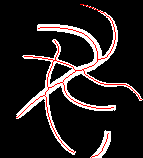
\includegraphics[height=1.5in]{imagenes/skel_in_segment.png}
	    \caption{Esqueletonizaci\'on representativa de la red sobre la imagen de \ref{Fig1b}.}
        \label{Fig1c}
    \end{subfigure}%
    ~ \hspace{0.5cm}
    \begin{subfigure}[t]{0.45\textwidth}
        \centering
        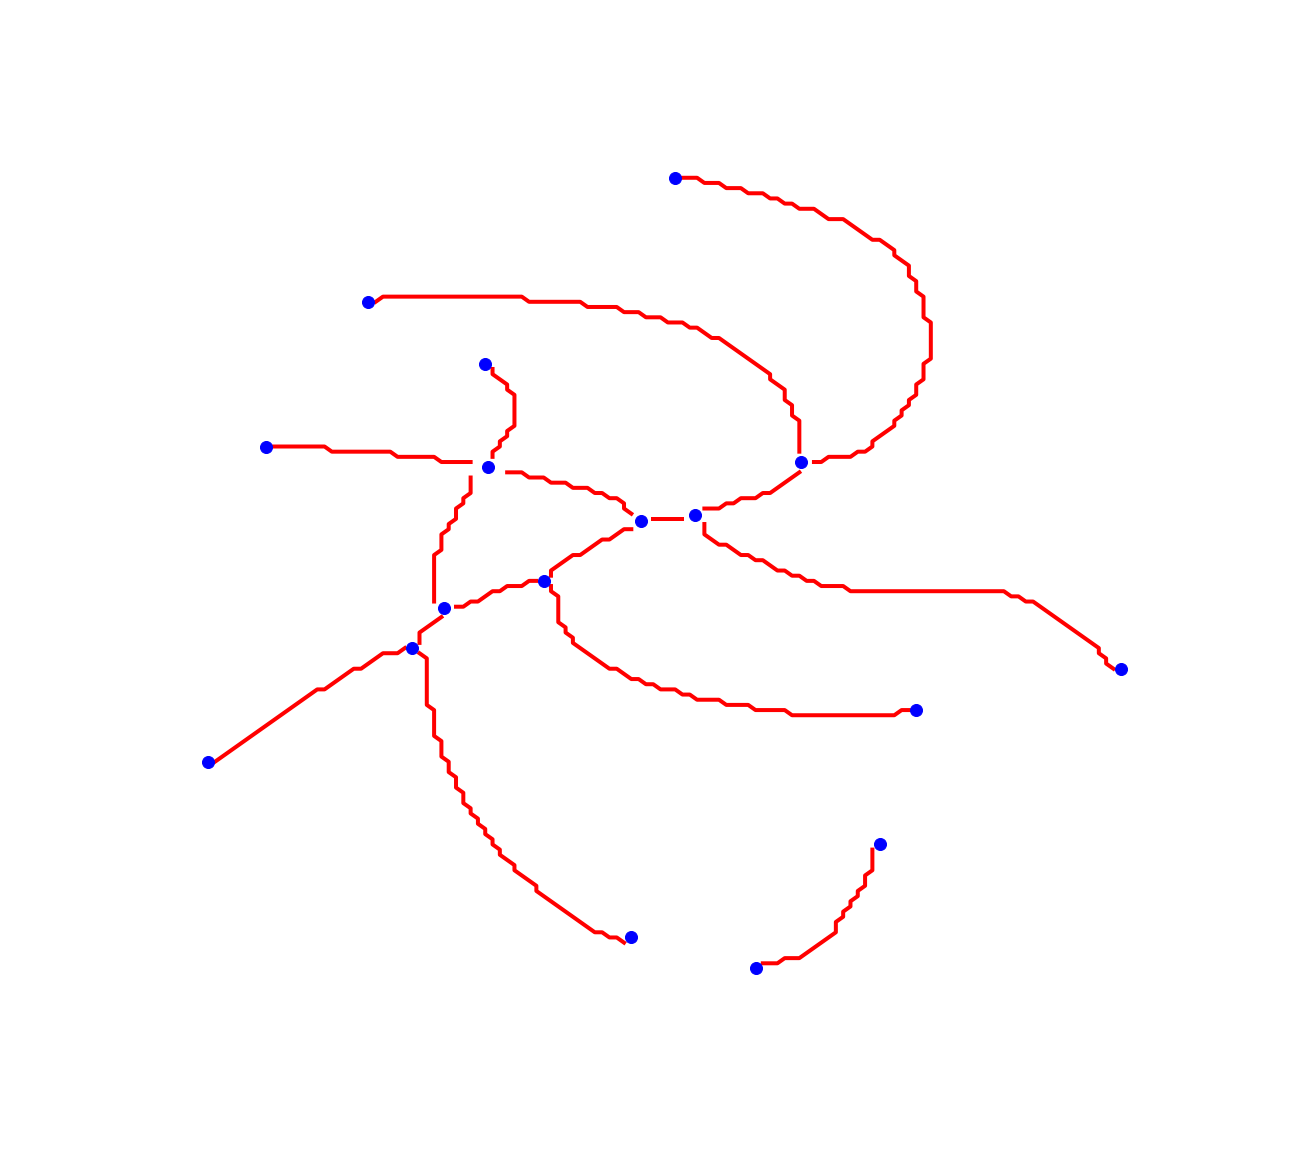
\includegraphics[height=1.5in]{imagenes/graph_of_skel_no_axis.png}
        \caption{Grafo que representa la esqueletonizaci\'on de la red.}
        \label{Fig1d}
    \end{subfigure}
%    \vskip\baselineskip
    \caption[Procedimiento para obtener un grafo que representa la red, utilizando segmentaci\'on y esqueletonizaci\'on.]{Procedimiento para obtener un grafo que representa la red, a partir del procesamiento de una imagen de microscop\'ia, utilizando segmentaci\'on y esqueletonizaci\'on. Fuente: \citet{breuer2015define}.}
\end{figure*}

Existen investigaciones en la literatura que apuntan a las distintas etapas de este problema, las que tienen en com\'un el uso de t\'ecnicas del \'area de procesamiento de im\'agenes de bajo nivel para el tratamiento inicial de la imagen de microscop\'ia. La individualizaci\'on de filamentos puede ser categorizada dependiendo si utiliza como enfoque primario herramientas de procesamiento de im\'agenes de bajo nivel, o si se aborda como un problema de optimizaci\'on. 
En ambas categor\'ias, las cr\'iticas m\'as repetidas en los trabajos del \'area suelen ser la cantidad de par\'ametros y la dificultad en su ajuste, en las diversas herramientas existentes. Un segundo problema com\'un es que la obtenci\'on de informaci\'on relacionada a la morfolog\'ia y el comportamiento de las redes es m\'as cualitativo que cuantitativo, como se indica en \citet{asgharzadeh2018computational} y en \citet{qiu2014quantitative}, lo que supone un problema al trasladar el  an\'alisis a una gran cantidad de datos, dado que cada enfoque es demasiado espec\'ifico a su correspondiente software.

\begin{figure*}[h]
    \begin{subfigure}[t]{0.5\textwidth}
        \centering
        
\includegraphics[height=1.2in]{imagenes/define-weighted-4-expected2.png}
        \caption{Visualizaci\'on de un resultado posible de individualizaci\'on, limitando los filamentos identificados a filamentos simples.}
        \label{Fig2a}
    \end{subfigure}
    ~ 
    \begin{subfigure}[t]{0.5\textwidth}
        \centering
        
\includegraphics[height=1.2in]{imagenes/define-weighted-4-expected1.png}
        \caption{Visualizaci\'on de otro resultado posible de individualizaci\'on, permitiendo filamentos m\'as complejos, como es el caso de filamentos con ramificaciones. }
        \label{Fig2b}
    \end{subfigure}
	\caption[Posibles resultados de la identificaci\'on de filamentos.]{Posibles resultados de la identificaci\'on de filamentos. Un planteamiento enfocado en un modelo de optimizaci\'on permitir\'a asociar las arista del grafo, como el de la figura \ref{Fig1d}, a uno o m\'as filamentos, entregando resultados como (a) o (b), expresado gr\'aficamente mediante gradiente de colores. Fuente: Elaboraci\'on propia.}
	%El resultado esperado de esta investigaci\'on es asociar a cada arista del grafo (como el de la figura \ref{Fig1d}) un peso que pondere diversos criterios como \'angulo de bifurcaci\'on del filamento, grosor y/o largo.
\end{figure*}

En resumen, el problema de identificar filamentos en im\'agenes de microscop\'ia esta limitado por la resoluci\'on, y los problemas de m\'ultiples par\'ametros a ajustar, para los m\'etodos basados en procesamiento de im\'agenes de bajo nivel, el costo computacional en los m\'etodos basados en optimizaci\'on, y falta de descriptores cuantitativos en ambas. La revisi\'on bibliogr\'afica da cuenta tambi\'en de pocas herramientas disponibles. Todo lo anterior implica que parte del an\'alisis deba ser manual, lo que para grandes cantidades de datos, hace los estudios m\'as propensos a errores. 

\section{Hip\'otesis y Objetivos}
Como se ha presentado, los m\'etodos de individualizaci\'on de filamentos que s\'olo usan herramientas de procesamiento de im\'agenes de bajo nivel, pueden representar la red a trav\'es de los filamentos que la conforman, sin embargo para realizar mediciones cuantitativas requieren ajustar m\'ultiples par\'ametros. Por otra parte los m\'etodos de optimizaci\'on permiten reducir los par\'ametros, pero con un alto costo computacional, el que puede ser abordado con el uso de heur\'isticas o algoritmos de aproximaci\'on. Tambi\'en se debe tener en consideraci\'on en ambos m\'etodos el n\'umero de caracter\'isticas utilizadas al momento de realizar la individualizaci\'on. Esto nos permite establecer la pregunta:

\smallskip
¿Es posible determinar correctamente la cantidad de filamentos, desarrollando un modelo de optimizaci\'on que utilice una combinaci\'on de m\'ultiples caracter\'isticas como el largo, grosor, \'angulo de bifurcaci\'on, curvatura o direcci\'on, tanto en la asignaci\'on de pesos como en la selecci\'on del subconjunto de caminos?
\smallskip

% costo computacional de m\'etodos de optimizaci\'on es abordado con algoritmos de aproximación o heurísticas
% Solucion actual propuesta en Define aborda el recorrido de grafos considerando como peso solo 1 valor que representa una caracteristica de la arista, 
% pregunta es si se puede determinar la cantidad de filamentos utilizando un peso que agrupe/pondere varias caracteristicas
%(geometricos comunmente)
% Entre las investigaciones y herramientas existentes derivadas de los mismos, 
%- overlap, intensidad, fragmentación


Al comenzar el proceso de individualizaci\'on de filamentos se desconoce el origen y fin de cada filamento, por lo que plantear un recorrido de grafos puede resultar computacionalmente costoso, lo que puede ser evitado al plantear un modelo de optimizaci\'on que pueda hacer la asociaci\'on entre aristas que sean parte del mismo filamento.

Se debe agregar que existe informaci\'on \textit{a priori}, indicada por el tipo de estructura observada, la cual restringe los comportamientos posibles de la red. Por ejemplo, los filamentos de prote\'ina actina no se pegan entre s\'i, formando estructuras sin ciclos, mientras que el ret\'iculo endoplasm\'atico (organelo celular encargado principalmente de la s\'intesis de prote\'inas) si presenta ciclos. Estas condiciones pueden aportar limites m\'as acotados a algunos de los criterios de cuantificaci\'on y es conocimiento disponible previo a la observaci\'on en el microscopio. Es importante destacar que alguna de la informaci\'on {\it a priori} corresponde a reglas emp\'iricas, que tambi\'en deben ser consideradas durante el an\'alisis.

En base a lo anterior, la hip\'otesis de esta investigaci\'on se basa en que a partir de un grafo con pesos, no dirigido, con o sin ciclos, que representa una red de filamentos, en conjunto con utilizar una combinaci\'on de caracter\'isticas de los segmentos de filamentos como largo, grosor, \'angulo de bifurcaci\'on o curvatura, sumado a la incorporaci\'on de informaci\'on previa disponible sobre el tipo de c\'elula (red de filamentos con o sin ciclos), es posible identificar a cada filamento en la red resolviendo un modelo de optimizaci\'on.

Para validar esta hip\'otesis, se propone realizar el siguiente objetivo general y los siguientes objetivos espec\'ificos:
\subsection{Objetivo General}
Desarrollar un modelo de optimizaci\'on para la individualizaci\'on de filamentos a partir de un grafo representativo de la red de filamentos, evaluando la variaci\'on en el resultado con distintas combinaciones entre las propiedades de cada segmento de filamento como el grosor, largo, \'angulo de bifurcaci\'on o direcci\'on.
%y que incorpore la informaci\'on {\it a priori} disponible

\subsection{Objetivos Espec\'ificos}
\begin{itemize}
    \item Generar un modelo de optimizaci\'on para la identificaci\'on de filamentos a partir de un grafo con pesos que representa la red de filamentos.
    \item Implementar un algoritmo que resuelva el modelo de optimizaci\'on, entregando como salida la identificaci\'on de filamentos, considerando casos de solapamiento y/o cruce.
    \item Identificar la ponderaci\'on de propiedades que entregue mejores resultados para grafos que representen una neurona, una bacteria y una c\'elula eucariota de planta.
    \item Evaluar t\'ecnicas en el estado del arte que realicen individualizaci\'on de filamentos.
    % usan s\'olo procesamiento de im\'agenes de bajo nivel como \citet{boudaoud2014fibriltool}, basada en poblaci\'on de p\'ixeles, o que utilizan un m\'etodo derivado de contornos activos, como \citet{xu2015soax}.
    %una soluci\'on exacta o aproximada respecto a la individualizaci\'on, dependiendo de la complejidad computacional del problema. 
\end{itemize}

%\subsubsection{Contribuci\'on}

% Contribuci\'on:
Como resultado de los objetivos planteados, se obtendr\'a una herramienta para el an\'alisis automatizado de estructuras de filamentos, lo que permitir\'ia mejorar el seguimiento de procesos din\'amicos o la identificaci\'on de procesos patol\'ogicos de forma autom\'atica.

\section{Estructura de esta tesis}
El capitulo \ref{chap:stateoftheart} resume el estado del arte de diversos aspectos relacionados a la individualizaci\'on de filamentos. El cap\'itulo \ref{sec:modeloOpti} define un modelo de optimizaci\'on que resuelve la identificaci\'on de filamentos, para el que se propone un algoritmo. Se presentan las m\'etricas y mediciones en el cap\'itulo \ref{chap:metodologia}. El cap\'itulo \ref{chap:res} presenta los resultados obtenidos para im\'agenes sint\'eticas e im\'agenes reales de distintas c\'elulas. Finalmente, en el cap\'itulo \ref{chap:conclu} se presentan las conclusiones.

%\begin{teo}
%Se tiene que $$\int_0^t e^sds=e^t-1.$$
%\end{teo}
%\end{intro}
\chapter{Antecedentes}
\label{chap:stateoftheart}
La individualizaci\'on de filamentos en una imagen es un problema derivado de la obtenci\'on de informaci\'on de filamentos en base a una imagen. Este \'ultimo ha ido variando a medida que la tecnolog\'ia en microscopios ha mejorado, lo que a su vez ha permitido el desarrollo de nuevos m\'etodos. Estos m\'etodos pueden a su vez diferir entre s\'i dependiendo del foco de la informaci\'on que buscan obtener a partir de la imagen, existiendo m\'etodos que se enfocan en reconstruir filamentos discontinuos, a la identificaci\'on de segmentos de filamento para la construcci\'on de las redes que estos conforman, o la individualizaci\'on en s\'i. Independientemente del objetivo de cada m\'etodo, es posible agruparlos en dos categor\'ias: M\'etodos basados en herramientas de visi\'on por computador y m\'etodos basados en optimizaci\'on. Los primeros realizan mayoritariamente operaciones de filtrado sobre la imagen, mientras que los segundos plantean parte de la obtenci\'on de la informaci\'on mediante la resoluci\'on de problemas de asignaci\'on o de minimizaci\'on de funciones.

Entre las herramientas disponibles para los m\'etodos basados en optimizaci\'on, se encuentra la metaheur\'istica {\it Ant Colony Optimization} (ACO), que se basa en el comportamiento de las hormigas al buscar alimento. Esta metaheur\'istica corresponde a la estrategia utilizada en esta investigaci\'on para individualizar filamentos.


\section{M\'etodos basados en herramientas de visi\'on por computador}
\label{sec:NonIndividualizationMethods}

La investigaci\'on de \cite{zhang2017extracting} identifica el problema de discontinuidad de filamentos en una imagen, pudiendo atribuirse esto a factores experimentales como la densidad del componente fluorescente, ruido u otras. En particular, el filamento analizado en esta investigaci\'on corresponde a microt\'ubulos. Para llevar a cabo la reconstrucci\'on de un filamento en base a segmentos, establecen el uso de dos filtros, denominados \textit{Filtro de Transformaci\'on Lineal} (LFT, Linear Filter Transformation) y \textit{Filtro de Transformaci\'on en base a la Orientaci\'on} (OFT, Orientation Filter Transformation). 
El filtro LFT busca resaltar caracter\'isticas lineales centr\'andose en cada p\'ixel y generando una serie de lineas con radio $r$, buscando la linea que contenga la mayor intensidad, seg\'un se observa en la Figura \ref{fig:MTLFT}. El filtro OFT complementa lo anterior, mediante un criterio de similaridad en la direcci\'on proyectada de los segmentos, un segundo criterio respecto a la distancia entre los extremos finales de cada segmento y un tercer criterio de continuidad, que limita el \'angulo entre el vector proyectado de un extremo y el vector que representa la distancia entre los extremos de cada segmento. Lo anterior se puede observar en la Figura \ref{fig:MTOFT}.

\begin{figure}[h]
        \centering
        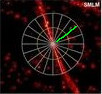
\includegraphics[scale=5]{imagenes/MT-LFT.jpeg}
        \caption[B\'usqueda por lineas con radio $r$ para diferentes \'angulos, según filtro LFT.]{B\'usqueda por lineas con radio $r$ para diferentes \'angulos, según filtro LFT. Fuente: \cite{zhang2017extracting}}.
        \label{fig:MTLFT}
\end{figure}

\begin{figure}[h]
        \centering
        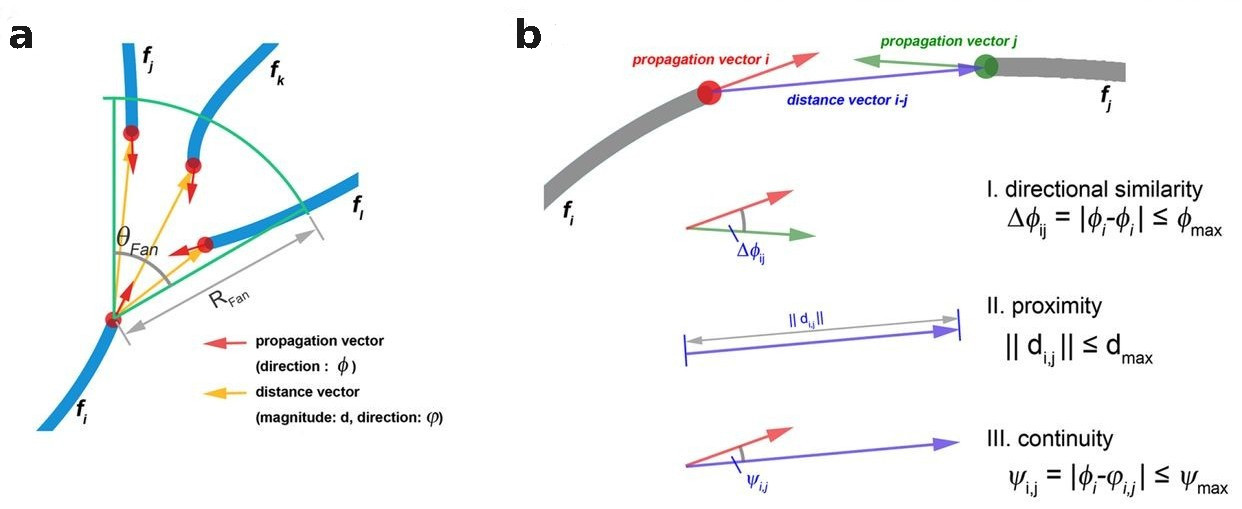
\includegraphics[scale=0.38]{imagenes/MT-OFT.jpeg}
        \caption[Criterios del filtro OFT.]{Criterios del filtro OFT: (a) Vectores de propagaci\'on (rojo) y distancia (amarillo) (b) Ejemplos de criterios de coincidencia de fragmentos de filamento I) Similaridad de direcci\'on, II) Proximidad, III) Continuidad. Fuente: \cite{zhang2017extracting}.}
        \label{fig:MTOFT}
\end{figure}


El fundamento de los criterios de OFT se basa en la asociaci\'on de las caracter\'isticas geom\'etricas como restricciones representativas del comportamiento mec\'anico de los microt\'ubulos. Uno de los objetivos de esta investigaci\'on es permitir el an\'alisis autom\'atico, dada las dificultades que presenta el an\'alisis manual de reconstrucci\'on. % es dificil hacer el analisis de forma manual
%asume non-branching filaments entonces soluciona el caso


% hablar de fibritool, Quantitave IFS y Aliosha
%fibritool
El trabajo de \cite{boudaoud2014fibriltool} conduce al desarrollo de {\it FibriTool}, un plugin para el software {\it ImageJ}, utilizado en an\'alisis cient\'ifico de im\'agenes. {\it FibriTool} calcula la orientaci\'on principal y la anisotrop\'ia de estructuras alargadas dentro de una regi\'on de inter\'es seleccionada manualmente. Para esto, utiliza el concepto de tensor nem\'atico, extra\'ido del comportamiento f\'isico de los cristales l\'iquidos. Espec\'ificamente, el tensor nem\'atico es la matriz sim\'etrica $n$ de $2\times2$ construida a partir de un vector unitario $t$, ecuaci\'on \ref{eq:fibritoolTensor}, definido en base a la derivada de primer orden de la intensidad del pixel en $x,y$. %Los componentes de $n$ se pueden observar en la ecuaci\'on \ref{eq:fibritoolComps}.

\begin{equation}
\label{eq:fibritoolTensor}
t = (t_x,t_y) = (
\dfrac{\partial I}{\partial y}, -\frac{\partial I}{\partial x}) / \sqrt{  
(\frac{\partial I}{\partial x})^2 + 
(\frac{\partial I}{\partial y})^2 }
\end{equation}

Luego, a partir de la matriz $n$ (ecuaci\'on \ref{eq:fibritoolComps}) se obtiene su primer vector propio $\Vec{e}_1$ que representa la orientaci\'on principal de los filamentos en el \'area de inter\'es, mientras que la diferencia de los valores propios $\lambda_1$ y $\lambda_2$ ($\lambda_1 > \lambda_2$), denominada $q = \lambda_1 - \lambda_2$, define la anisotrop\'ia.


\begin{equation}
n =
\begin{bmatrix}
(t_x)^2 & t_x \times t_y \\
t_x \times t_y & (t_y)^2 
\end{bmatrix}
\label{eq:fibritoolComps}
\end{equation}

% \begin{subequations}
% Componentes de $n$ para el tensor nem\'atico:
% \begin{align}
%     n_x,x &= (t_x)^2 \\
%     n_y,y &= (t_y)^2 \\
%     n_x,y &= n_y,x = t_x \times t_y
% \end{align}
% \end{subequations}
Los autores de {\it FibriTool} desarrollan este m\'etodo para evitar el uso de derivadas de segundo orden, que presentan sensibilidad al ruido, necesitando de pasos previos en la limpieza de la imagen.

\begin{figure}[h!]
        \centering
        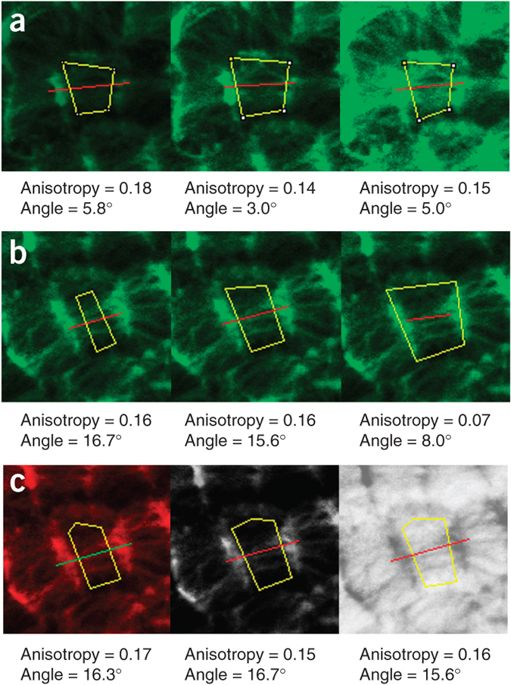
\includegraphics[scale=0.6]{imagenes/fibritool.jpg}
        \caption[\'Area de inter\'es seleccionada manualmente en amarillo, y resultado de FibriTool en rojo o verde.]{\'Area de inter\'es seleccionada manualmente en amarillo, y resultado de FibriTool en rojo o verde. Fuente: \cite{boudaoud2014fibriltool}.}
        \label{fig:fibritool}
\end{figure}

% Quantitative IFS
Una investigaci\'on que propone la individualizaci\'on de segmentos de filamentos es \cite{qiu2014quantitative}, la que plantea un filtro de detecci\'on de caracter\'isticas de 6 pasos m\'as un algoritmo llamado \textit{SBDA} que busca eliminar segmentos de filamentos menores a 2 p\'ixeles (Figura \ref{fig:IFS}). La individualizaci\'on de segmentos de filamentos entrega informaci\'on morfol\'ogica de un segmento con respecto a su entorno, se\~nalando si se encuentra en estado de aislaci\'on, intersectado, bifurcado o en superposici\'on con otro segmento de filamento.

%describir filtros, intensidad es con fibre coefficient
Las 6 etapas del filtro consideradas en este m\'etodo consisten en 4 etapas de an\'alisis de la imagen y 2 de an\'alisis topol\'ogico que se resumen en lo siguiente:

\begin{enumerate}
    \item Depuraci\'on de la imagen: El primer filtro comienza por reducir el ruido y realzar el contraste de la imagen, aumentando la intensidad de los p\'ixeles que est\'en sobre un umbral, al mismo tiempo que eliminan los p\'ixeles que se encuentren debajo del mismo umbral.
    \item Filtro de informaci\'on estructural: El segundo paso consiste en filtrar informaci\'on estructural, que se basa en los valores propios de la matriz Hessiana, buscando descartar objetos en la imagen que no correspondan a una figura tubular.
    \item Eliminaci\'on de se\~nales d\'ebiles: El tercer filtro ejecuta una limpieza de estructuras con una intensidad baja y/o aisladas, de las que puede concluirse que no corresponden a elementos en el plano focal de inter\'es.
    \item Generaci\'on de esqueleto: Finalmente dentro del an\'alisis sobre la imagen, el filtro de esqueletonizaci\'on realiza un adelgazamiento de la imagen, en el que cada estructura pasa a tener 1 p\'ixel de ancho, facilitando el an\'alisis topol\'ogico posterior.
    \item Clasificaci\'on topol\'ogica y algoritmo SBDA: Consiste en el an\'alisis a nivel de p\'ixel y su vecindario de 8 p\'ixeles alrededor para determinar si este corresponde a un punto aislado, al final de un fragmento de filamento, a un punto interior de un filamento, o a una junci\'on de filamentos. Seguido de aquello, el algoritmo SBDA realiza otro an\'alisis topol\'ogico a nivel de p\'ixel que borra los segmentos menores a 3 p\'ixeles, adem\'as de realizar los calculos de distancia de cada segmento/fragmento.
    \item Reconstrucci\'on: Para finalizar el an\'alisis topol\'ogico y el proceso de filtrado, se lleva a cabo una combinaci\'on de segmentos para construir los filamentos bas\'andose en el par\'ametro $W$, llamado \textit{ancho efectivo}, cuyo valor define si la uni\'on de 2 o m\'as segmentos se trata de una bifurcaci\'on, una intersecci\'on o un solapamiento. 
\end{enumerate}

\begin{figure}[h!]
        %\centering
        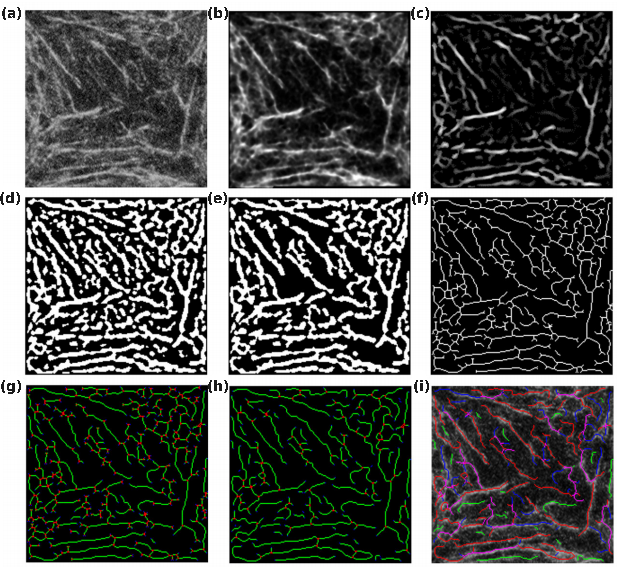
\includegraphics[scale=0.75]{imagenes/QuantitativeIFS.png}
        \caption[Etapas de individualizaci\'on de filamentos de \cite{qiu2014quantitative}.]{Etapas de individualizaci\'on de filamentos de \cite{qiu2014quantitative}. (a): Imagen de red de fibras de un osteoblasto. (b, c, d, e, f): Filtros de limpieza, tubularidad, segmentaci\'on, conectividad y esqueletonizaci\'on. (g): Clasificaci\'on topol\'ogica de intersecciones a nivel de p\'ixel. (h): Resultado de algoritmo SBDA. (i): Individualizaci\'on de segmentos de filamentos seg\'un forma estructural: aislado (verde), solapado (morado) u otro (azul). Fuente: \cite{qiu2014quantitative}.}
        \label{fig:IFS}
\end{figure}
%describir SBDA, el analisis es a nivel de pixel

% se mide caracteristicas geometricas, como largo, distribucu\'on de la orientaci\'on, y como los resultados son afectados por el ruido.
Como resultados de \cite{qiu2014quantitative}, adem\'as de la informaci\'on morfol\'ogica, se obtienen caracter\'isticas geom\'etricas como el largo de los segmentos de  filamentos y la distribuci\'on de la orientaci\'on de los segmentos, as\'i como el cambio de estos valores para variaciones en la relaci\'on entre la se\~nal y el ruido de la imagen.


\smallskip
La investigaci\'on de \cite{alioscha2016robust} presenta un marco para el an\'alisis de im\'agenes con la finalidad de identificar filamentos de actina, mediante una combinaci\'on de filtros con un algoritmo de uni\'on de segmentos. La propuesta inicial se basa en que una imagen puede ser separada en 3 componentes: el fondo o {\it background} de la imagen, los filamentos y el ruido. Para obtener la imagen que contiene los filamentos y descartar en mayor medida el ruido, los autores utilizan la libreria MCALab en MATLAB. Luego, buscan intensificar los p\'ixeles que corresponden a los filamentos, para lo cual aplican 3 filtros: un filtro Gaussiano, un filtro Laplaciano y un filtro Gaussiano direccional, obteniendo como resultado lo que se muestra en la Figura \ref{fig:AlioshaRobust}.

\begin{figure}[t]
    \centering
    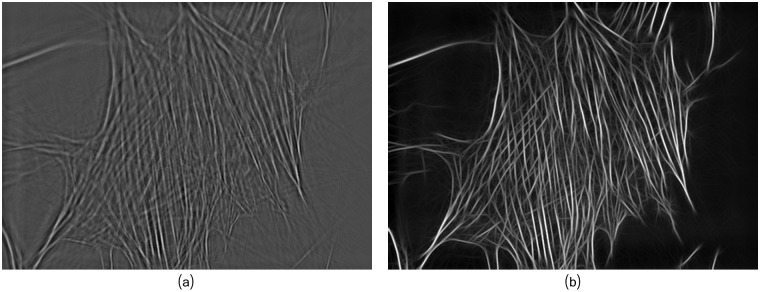
\includegraphics[scale=2]{imagenes/Aliosha2016-GaussLaplFilters.jpg}
    \caption[Aplicaci\'on de filtros posterior a la segmentaci\'on.]{A partir de la segmentaci\'on obtenida con la libreria MCALab (a), se aplican los filtros Gaussiano, Laplaciano y Gaussiano direccional para obtener una intensificaci\'on de los filamentos (b). Fuente: \cite{alioscha2016robust}.}
    \label{fig:AlioshaRobust}
\end{figure}

El paso siguiente es la aplicaci\'on de un detector de l\'ineas multi-escala, que busca determinar la pertenencia de un p\'ixel a una l\'inea, que varia su grosor y \'angulo dependiendo del tama\~no/escala del vecindario elegido. Las l\'ineas var\'ian en su grosor $s \in [1,W]$, con $W$ el grosor esperado de una fibra de actina, as\'i como en su \'angulo, que varia de forma discreta entre 0 y 180\textdegree. El detector de l\'ineas asigna una puntuac\'on que determina la probabilidad del p\'ixel a pertenecer a una de las l\'ineas. Lo anterior entrega como resultado candidatos de segmentos de l\'ineas. Para elegir a un candidato como segmento de l\'inea definitivo, la idea principal es recorrer los p\'ixeles en secuencia y ajustar las l\'ineas candidatas usando el m\'etodo de m\'inimos cuadrados hasta que un umbral de error es sobrepasado. Por cada vez que se sobrepasa el umbral de error, se comienza la elecci\'on de un nuevo segmento de l\'inea para los p\'ixeles que siguen. Si el candidato de segmento de l\'inea tiene un largo $l < L$, se descarta. $L$ es un par\'ametro definido emp\'iricamente.
% esto arroja candidatos de segmentos de lineas -> elegir segmentos de l\'ineas
% despues hay merge de segmentos lineas -> segmentos de filamentos, fibras en este caso

Finalmente, para construir las fibras de actina, los segmentos de l\'inea elegidos en el paso anterior son unidos entre si mediante una ventana de largo $L$, en la que 2 segmentos de l\'inea se superpongan y no tengan una diferencia entre sus \'angulos mayor al umbral $T_{\theta}$. 
%\cite{asgharzadeh2018computational}

Otras investigaciones similares que siguen un enfoque basado principalmente en herramientas de visi\'on por computador son \cite{doi:10.1021/ma502264c}\cite{lichtenstein2003quantitative}\cite{asgharzadeh2018computational}. En general, los trabajos desarrollados bajo este enfoque requieren del uso o sintonizaci\'on de m\'ultiples par\'ametros.


%la dificultad para identificar correctamente un filamento de otro, en los casos de  superposici\'on, fragmentaci\'on, o variaciones de intensidad en la imagen...


\section{M\'etodos basados en optimizaci\'on}
\label{sec:OptiMethods}
En la segunda categor\'ia, \cite{cerda2014geometrical} plantea la identificaci\'on de segmentos de filamentos como un problema de asignaci\'on, utilizando las medidas de distancia euclidiana y angular como restricciones, y el algoritmo h\'ungaro para su resoluci\'on.
%SOAX, extraccion y cuantifiacion de la red
Por su parte, la investigaci\'on de \cite{xu2015soax} llamada SOAX, emplea curvas param\'etricas de contorno abierto (SOAC, {\it Stretching Open Active Contour}) en conjunto con una funci\'on de minimizaci\'on para obtener un grupo acotado de redes de filamentos, entre las que el usuario puede elegir una, con la finalidad de realizar un an\'alisis posterior. Las curvas param\'etricas de contorno abierto son reguladas por 2 par\'ametros: $\tau$, que fija el umbral de intensidad desde el que se inicializa una SOAC, lo que entrega los puntos de intensidad m\'aximos locales de la imagen para la inicializaci\'on. El segundo par\'ametro, $K_{str}$, es el factor que regula la elongaci\'on/evoluci\'on de cada SOAC. Una vez concluida la inicializacio\'on y evoluci\'on de curvas SOAC, se identifican las junciones/intersecciones generadas entre diversas curvas SOAC, agrup\'andose seg\'un su cercan\'ia. Lo anterior se puede observar en la Figura \ref{fig:SOAX}.

\begin{figure}[h]
        %\centering
        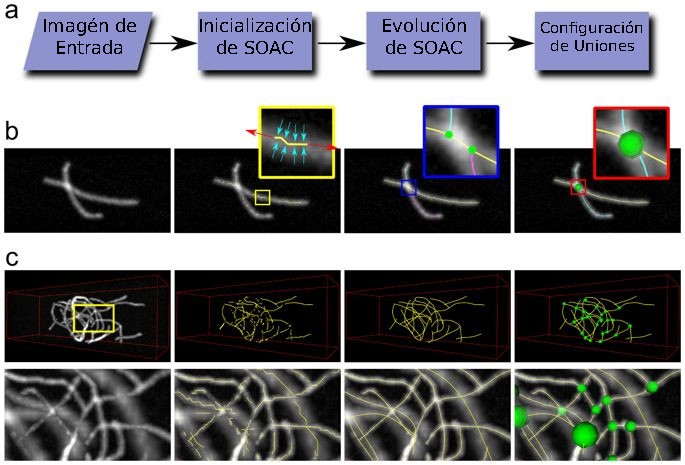
\includegraphics[scale=0.7]{imagenes/SOAX_translated.jpg}
        \caption[Etapas de SOAX.]{Etapas de SOAX: A partir de los puntos de alta intensidad se inicializan curvas param\'etricas de contorno abierto (SOAC), las que crecen, generando intersecciones entre ellas. Finalmente, se agrupan las intersecciones más cercanas. Fuente: \cite{xu2015soax}.}
        \label{fig:SOAX}
\end{figure}

La funci\'on de minimizaci\'on que los autores denominan como  \textit{F-Function}, $F = -L_{total} + {c}\cdot L_{<t}$, se encuentra definida por otros 2 par\'ametros: el factor $c$ ($c > 1$) que regula la penalizaci\'on de las SOACs con bajo \textit{Signal to Noise Ratio (SNR)}, y el umbral $t$, que define el valor mínimo de SNR necesario para no descartar una SOAC. El umbral $t$ se ve reflejado en $L_{<t}$ dentro de la \textit{F-Function}, como el largo de SOACs en una regi\'on de la imagen con SNR por debajo de $t$, y que ser\'an penalizados dado que son calificados como de baja certeza. $L_{total}$ representa el largo total de las SOACs en el resultado final.

% \begin{equation}
%   \label{eq:FFunction}
%     F = -L_{total} + {c}\cdot L_{<t} 
% \end{equation}


En esta categor\'ia tambi\'en se incluye \cite{breuer2015define}, que en base a un grafo no dirigido con pesos que representa la red de filamentos, realiza la individualizaci\'on de estos. El uso de un grafo como dato de entrada permite representar a cada filamento mediante un conjunto de aristas adyacentes en el grafo. Esto permite que la b\'usqueda e individualizaci\'on de filamentos, con un segmento de filamento representado por una o m\'as aristas del grafo, sumado a las restricciones que plantea el autor, sea tratado como un problema de {\it Set Cover} \cite{caprara2000algorithms}. La definici\'on de {\it Set Cover} es:

\begin{quote}
Dado un conjunto de elementos, denominado universo, y $n$ conjuntos cuya unión comprende el universo, el {\it Set Cover Problem} consiste en identificar el menor n\'umero de conjuntos cuya unión a\'un contiene todos los elementos del universo.
\end{quote}

%En particular, el m\'etodo {\it FCP} presentado en la secci\'on \ref{Antecedentes}, utiliza s\'olo el grosor como caracter\'istica en la etapa de asignaci\'on de pesos a las aristas del grafo, lo que es usado en la funci\'on de minimizaci\'on del problema de optimizaci\'on planteado por ellos. En la etapa de selecci\'on del subconjunto de caminos, el mismo m\'etodo desarrolla una heur\'istica que utiliza {\it BFS} en conjunto con el \'angulo de deflexi\'on entre aristas. El mismo m\'etodo evita realizar un recorrido de grafos, al buscar las combinaciones de caminos del subconjunto P' que dan lugar a uno o m\'as filamentos mediante la minimizaci\'on de un {\it Set Cover}. 

%representa un camino en este grafo, y los conjuntos de caminos 
\medskip
%Todos estos enfoques, cuya entrada principal de datos son las im\'agenes etiquetadas a trav\'es de marcadores fluorescentes, 
% basados en grafos

El programa \texttt{DeFine} desarrollado en \cite{breuer2015define} describe el problema de individualizaci\'on de filamentos como un problema de b\'usqueda de conjuntos de aristas en un grafo. En esta investigaci\'on, un filamento es representado por un conjunto de aristas, denominado como un camino. Los autores de esta investigaci\'on se basan inicialmente en un problema del tipo {\it Path Cover} \cite{ntafos1979path}, extendiendo la definici\'on de {\it Path Cover} mediante la asignaci\'on de un peso a cada segmento/arista del grafo, para calcular la {\it aspereza} o diferencia de homogeneidad en un camino. El c\'alculo del peso a lo largo de un camino es lo que permite individualizar filamentos, siendo el peso un reflejo del grosor o intensidad de una arista.
%, o tambi\'en puede ser calculado respecto al \'angulo entre aristas.
Este problema particular es llamado {\it Filament Covering Problem} (FCP) y los autores demuestran que es NP-Hard, por lo que proponen un algoritmo de aproximaci\'on mediante {\it Set Cover}, cuyo objetivo es que cada arista pertenezca al menos a un camino (conjunto de aristas).

La adaptaci\'on a lo definido por {\it FCP} es: 
\begin{quote}
Sea el universo $U$ conformado por las aristas del grafo, y un conjunto $S$, conformado por conjuntos de aristas, cada uno con costo $c_s$, $s \in S$:

Encontrar un subconjunto $S_{set} \subseteq S$ con costo m\'inimo (o promedio, dependiendo de la forma en que se calcula la aspereza) tal que cada elemento en $U$ este cubierto al menos una vez.
\end{quote}

Los autores de DeFine demuestran que el FCP es NP-Hard en grafos, debido a la relaci\'on entre el n\'umero de nodos y el conjunto total de caminos posibles. Esta relaci\'on implica que al aumentar el n\'umero de nodos, el conjunto total de caminos en un grafo, definido como $P$, crece de forma exponencial. Para esta situaci\'on, los autores de DeFiNe prueban que el FCP en \'arboles es soluble en tiempo polinomial, bas\'andose en \cite{lin2006vertex}. La complejidad computacional para resolver el FCP en \'arboles es de $\mathcal{O}(n^{4})$ para caminos que no comparten nodos o aristas, es decir, no se superponen. Para permitir caminos que se superponen se agrega el par\'ametro $k$ que define el n\'umero m\'aximo de superposiciones de caminos en una arista, quedando la complejidad computacional igual a $\mathcal{O}(n^{2k+2})$.


%aca entran las formas de obtener esos arboles simples y bosques, con las heuristicas de define
DeFine propone 2 heur\'isticas para construir \'arboles de los cuales se puedan extraer un subconjunto $P' \in P$ representativo de caminos simples: recorrer el grafo por su anchura ({\it Breadth-First Search}), deteni\'endose al momento en que el \'angulo de deflexi\'on entre aristas adyacentes supere los 60\degree, o generar caminos a partir de 100 \'arboles de expansi\'on m\'inima aleatoria ({\it RMST}), aportando cada uno con $N(N-1)/2$ caminos no triviales y sin direcci\'on. 


El subconjunto $P'$ constituye los datos de entrada del problema de {\it Set Cover}, el que se resuelve a trav\'es de un algoritmo de aproximaci\'on lineal fraccional binario \cite{breuer2015define}, en el que al subconjunto $P'$ se le aplica la funci\'on objetivo, para encontrar los miembros de $p \in P'$ que mejor minimicen la diferencia de homogeneidad en sus caminos. La restricci\'on de lo anterior es que cada arista del grafo pertenezca a lo menos a un camino. El flujo de decisiones para generar el subconjunto de caminos puede observarse en la Figura \ref{fig:define-set-cover}.

\begin{figure*}[h]
    \centering
    \label{fig:flujo-expected}
    \begin{subfigure}[t]{\textwidth}
        \centering
        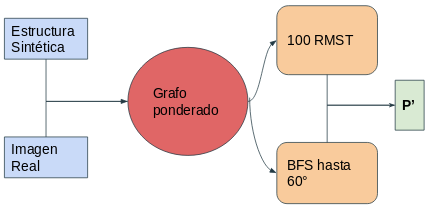
\includegraphics[scale=0.5]{imagenes/flujoDefine.png}
        \caption{Entrada de datos y elecci\'on de subconjunto de caminos {\bf P'} en DeFine.}
        \label{fig:define-set-cover}
    \end{subfigure}%
    \vskip\baselineskip
    \begin{subfigure}[t]{\textwidth}
        \centering
        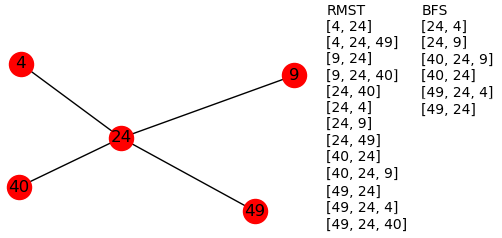
\includegraphics[scale=0.8]{imagenes/BFSvsRMSTpaths.png}
        \caption{Subconjunto {\bf P'} para el grafo de 5 nodos a la izquierda, utilizando la opci\'on de 100 {\it RMST} o heur\'istica de {\it BFS} que corta el camino al encontrar un \'angulo de deflexi\'on mayor a 60\degree entre aristas adyacentes.  }
        \label{fig:subconjunto-p-prima-caminos-posibles}
    \end{subfigure}
    \caption[Extracci\'on de caminos para formar P' en DeFiNe.]{(a) A partir de un grafo ponderado proveniente de una estructura sint\'etica o de una imagen real, se elige {\bf P'} entre los $N(N-1)/2$ caminos no triviales y sin direcci\'on que aporta cada uno de los 100 \'arboles de expansi\'on m\'inima aleatoria ({\it RMST}), o los caminos resultantes de la heur\'istica de b\'usqueda por anchura ({\it BFS}) con interrupci\'on al dar con una arista que tenga un \'angulo superior a 60\degree. (b) Subconjunto {\bf P'} de P, para el grafo de 5 nodos de ejemplo a la izquierda. Fuente: \cite{breuer2015define}.}
    \end{figure*}
    
    
%Este enfoque faculta que al tener un grafo que representa la red de filamentos, como en la figura \ref{Fig1d}, sea posible llegar a resultados como los que aparecen en las figuras \ref{Fig2a} o \ref{Fig2b} a trav\'es de la minimizaci\'on de la diferencia de homogeneidad del peso de las aristas en un camino, y de restricciones a las uniones entre las mismas. 

Cabe destacar que el {\it FCP} s\'olo utiliza 2 caracter\'isticas independientes para describir los segmentos de los filamentos, siendo el \'angulo de deflexi\'on entre aristas usado en la etapa de selecci\'on de subconjuntos de caminos s\'olo si es seleccionada la heur\'istica {\it BFS}, y el grosor o intensidad, empleado para describir el peso de las aristas. En el caso de la heur\'istica de {\it RMST}, se asignan pesos aleatorios uniformemente distribuidos a las aristas, por lo que no hay uso de caracter\'isticas asociadas a los filamentos.



En el caso de los m\'etodos basados en optimizaci\'on, la mayor cr\'itica es su costo computacional, el que aumenta a medida que se complejiza, limitando en parte aquel enfoque. Se debe agregar que los par\'ametros utilizados por estas t\'ecnicas (\'angulos o  distancias m\'aximas entre filamentos) son complejas de obtener de los expertos directamente. Sin embargo, una de sus ventajas es que automatizan la recuperaci\'on de informaci\'on incluyendo una mayor cantidad de propiedades a cada arista. 


%resolucion, cantidad parametros, descriptores, costo computacional
En resumen, el problema de identificar filamentos en im\'agenes de microscop\'ia esta limitado por la resoluci\'on, y los problemas de m\'ultiples par\'ametros a ajustar, para los m\'etodos basados en procesamiento de im\'agenes, el costo computacional en los m\'etodos basados en optimizaci\'on, y falta de descriptores cuantitativos en ambas. La revisi\'on bibliogr\'afica da cuenta tambi\'en de pocas herramientas disponibles. Todo lo anterior implica que parte del an\'alisis deba ser manual, lo que para grandes cantidades de datos, hace los estudios m\'as propensos a errores. 


\section{Generaci\'on de un grafo desde una imagen}
\label{sec:genGrafFromImage}
%La falta de herramientas analíticas para cuantificar las estructuras sigue siendo un cuello de botella, ya que el análisis manual de grandes conjuntos de datos requiere una gran cantidad de tiempo y son propensos a sesgos y errores.
%Por otra parte, la soluci\'on a problemas de superposici\'on se soluciona mediante la sintonizaci\'on de par\'ametros, los que var\'ian dependiendo de la c\'elula observada. En el caso del uso de \textit{thinning} en una imagen, la informaci\'on respecto al grosor de la estructura se pierde.
El uso de grafos para la individualizaci\'on de filamentos implica la necesidad de obtener el grafo a partir de una imagen para luego realizar su an\'alisis. Algunas de las dificultades involucradas en la obtenci\'on de un grafo se relacionan al ruido y la resoluci\'on de la imagen. Un ejemplo de aquello se observa en la Figura \ref{fig:NoConsensoGeneral}.

\begin{figure*}[h]
    \begin{tabular}{c c c}
        \multirow[c]{2}{*}[2.5cm]{
        \begin{subfigure}[t]{0.4\textwidth}
        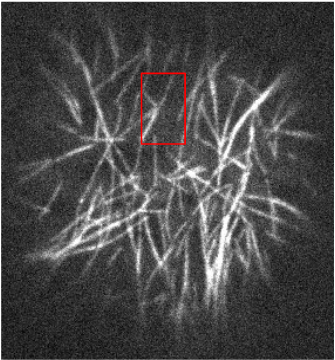
\includegraphics[scale=0.5]{imagenes/NoConsenso.png}
        \caption{Microt\'ubulos en planta {\it Marchantia}.\\Fuente: Paula Llanos}
        \label{fig:NoConsensoGeneral}
        \end{subfigure}  
        }
        &
        \multirow[c]{2}{*}[2cm]{
        \begin{subfigure}[t]{0.25\textwidth}
        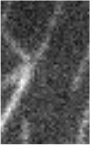
\includegraphics[]{imagenes/NoConsenso2.png}
        \caption{Secci\'on resaltada en rojo de (a)} %\ref{fig:NoConsensoGeneral}
        \label{fig:NoConsensoRect}
        \end{subfigure}
        }
        &
        \begin{subfigure}[t]{0.21\textwidth}
        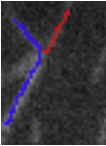
\includegraphics[scale=0.8]{imagenes/NoConsenso3.png}
        \caption{Opci\'on 1 de microt\'ubulos en (b)} %\ref{fig:NoConsensoRect}
        \label{fig:NoConsensoOpcion1}
        \end{subfigure} \\
        & &
        \begin{subfigure}[b]{0.21\textwidth}
        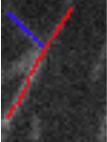
\includegraphics[scale=0.8]{imagenes/NoConsenso4.png}
        \caption{Opci\'on 2 de microt\'ubulos en (b)}
        \label{fig:NoConsensoOpcion2}
        \end{subfigure} \\
    \end{tabular}
    
    \caption[Dificultad de individualizaci\'on que enfretan los expertos al analizar manualmente una imagen de filamentos.]{Dificultad de individualizaci\'on que enfretan los expertos al analizar manualmente una imagen de filamentos, en particular, microt\'ubulos. Fuente: Elaboraci\'on Propia.}
    \label{fig:NoConsenso}
\end{figure*}

%El ruido en una imagen y la resoluci\'on de la misma son aspectos que pueden perjudicar la obtenci\'on de un grafo a partir de una imagen. 
Mientras que el ruido ha sido estudiado en la literatura, el problema de resoluci\'on depende principalmente de la capacidad del microscopio que se utilice. El l\'imite m\'aximo de resoluci\'on, denominado $\lambda/2$, determina el tama\~no m\'inimo que 2 objetos que se encuentren juntos pueden tener para no observarse como un \'unico elemento. Lo anterior sucede para algunos tipos de filamentos como los microt\'ubulos que pueden medir tan solo 25 nan\'ometros, lo que se encuentra por debajo de $\lambda/2$ para diversos microscopios.


Un problema derivado de la resoluci\'on de una imagen en la que se observan filamentos yace en que 2 expertos pueden disentir al realizar una individualizaci\'on manual de filamentos, como se indica en las figuras \ref{fig:NoConsensoOpcion1} y \ref{fig:NoConsensoOpcion2}. Esta discrepancia implica que para algunos tipos de c\'elulas donde se observen filamentos no es posible conocer a priori el origen y el final de un filamento. Adicionalmente, se presenta una dificultad en la representaci\'on de un filamento en un grafo, ya que esta se basa en un conjunto de aristas adyacentes, lo que lleva a tener un universo de hasta $n!$ posibles combinaciones en el espacio de soluciones. Cada conjunto de aristas adyacentes que representa a un filamento se denomina camino o recorrido.


La extracci\'on de un grafo a partir de una imagen, consiste en extraer un grafo $G = (V,E)$ de una imagen tal que $G$ sea un grafo simple, no dirigido, ponderado, conectado o desconectado, con o sin ciclos. Esto implica que exista a lo m\'as 1 arista por cada par de nodos adyacentes, prohibi\'endose la existencia de nodos conectados consigo mismos. Es importante evitar que $G$ sea un grafo completo, dado que con $n$ nodos/v\'ertices $G$ llega a tener $\frac{n(n-1)}{2}$ aristas.
Se definen los v\'ertices/nodos del grafo $G$ como $V(G)$ y las aristas de $G$ como $E(G)$. 
Que el grafo $G$ sea ponderado implica que para las aristas del grafo ($E(G)$), existen caracter\'isticas asociadas que se expresan como caracter\'isticas geom\'etricas, topol\'ogicas, espaciales y/u otras.
%$\forall e \in \quad E(G) \quad  \exists $ 


La importancia del procedimiento de extraci\'on o generaci\'on de un grafo que representa una red de filamentos a partir de una imagen radica en que define la cantidad de informaci\'on disponible para llevar a cabo la individualizaci\'on de filamentos. A partir de una imagen es posible obtener una cantidad de caracter\'isticas de distinta \'indole, lo que permite en etapas posteriores clasificar de diversas formas nodos, aristas, de forma aislada o en conjuntos, efectivamente disminuyendo el espacio de b\'usqueda. Con las herramientas actuales disponibles en la literatura, es posible realizar la extracci\'on de una red de filamentos con algún nivel de informaci\'on como en \cite{xu2015soax}. Sin embargo, las transformaci\'on de aquella red a un grafo, as\'i como la incorporaci\'on de las caracter\'isticas y/o propiedades hacia el grafo son un procedimiento no automatizado, por lo que el esfuerzo que el experto debe realizar es cercano a individualizar los filamentos de manera manual.

A partir de las investigaciones en la literatura, es posible agrupar los m\'etodos para extraer la informaci\'on que permite la construcci\'on de un grafo a partir de una imagen, como lo son los nodos y las aristas, en dos conjuntos: los que se basan en esqueletonizaci\'on \cite{lavado2018comparacion} y los que no. 

\subsection{Extracci\'on de un Grafo mediante Esqueletonizaci\'on}
\label{subsec:infoLossSkel}

%Que es la skeletonizacion y como extrae el grafo. Uso de liberia sknw
Los m\'etodos basados en esqueletonizaci\'on consisten primariamente en la reducci\'on de los p\'ixeles pertenecientes al plano de inter\'es o {\it foreground} en una imagen binaria, hasta formar una representaci\'on del objeto en la imagen de 1 p\'ixel de ancho. El proceso debe mantener la conectividad del objeto adelgazado y a su vez, reducir la dimensi\'on del objeto en la imagen para facilitar su an\'alisis \cite{saha2017skeletonization}. Un an\'alisis de los vecindarios de los p\'ixeles del esqueleto construido es una de las formas m\'as sencillas en que se puede distinguir si un p\'ixel representa un nodo o si es parte de un arista. Una librer\'ia que realiza tal an\'alisis es {\it skan} \cite{nunez2018new}, entregando estad\'isticas del grafo extra\'ido como largo promedio de una rama del esqueleto (equivalente a una arista del grafo), tipo de rama, curvatura de una rama, entre otras mediciones. Sin embargo, el formato de salida del grafo para esta herramienta corresponde a {\it Compressed sparse row} o CSR, lo que causa que un an\'alisis de mayor profundidad o el paso del grafo a una herramienta de individualizaci\'on de filamentos necesite de una librer\'ia adicional. 


Otra herramienta que realiza un an\'alisis similar para obtener un grafo a partir de un esqueleto es {\it sknw}, parte del framework {\it ImagePy} \cite{wang2018imagepy}. La diferencia propuesta por {\it sknw} radica en que se integra con la librer\'ia {\it NetworkX} \cite{hagberg2008exploring}, utilizando la estructura de datos para grafos que esta \'ultima posee para elegir entre m\'ultiples formatos de salida. Aquello otorga flexibilidad en la integraci\'on de herramientas que utilizan como base el grafo para realizar an\'alisis posteriores, como es el caso de la individualizaci\'on de filamentos.

% se puede extraer el skeleton con librerias en varios lenguajes, como octave, matlab o python (usando scipy). La opci\'on se encuentra en la secci\'on de herramientas morfol\'ogicasd de cada uno. De ahi al grafo, se puede utilizar un procedimiento que haga an\'alisis de vecindarios de p\'ixeles como \cite{qiu2014quantitative}

%problema de skeleton
Independiente de la herramienta usada para obtener la informaci\'on topol\'ogica de la c\'elula observada, el procedimiento de esqueletonizaci\'on puede sufrir de p\'erdida de informaci\'on, dado que mediante el o los pasos de adelgazamiento, puede existir p\'erdida de la informaci\'on de los vecinos de los p\'ixeles que conforman el esqueleto obtenido. Esta informaci\'on puede ser relativa a aspectos geom\'etricos como el ancho, o servir como los datos de entrada para calcular informaci\'on derivada mediante m\'etodos como {\it image moments} \cite{flusser2009moments}\cite{chaumette2004image}.

% mencionar superpixels y describir que son citando a 
Una forma de obtener la informaci\'on de vecindario mencionada es siguiendo la idea de agrupaci\'on de p\'ixeles similares o cercanos utilizada en superpixeles \cite{achanta2012slic}. Los algoritmos de generaci\'on de superpixeles juntan conjuntos de p\'ixeles para obtener nuevas unidades at\'omicas sobre las cuales se realiza el an\'alisis, reduciendo la complejidad de este. El prop\'osito de basarse en la idea de superpixeles y no en el concepto de forma completa se fundamenta en que no se busca generar una segmentaci\'on acabada, sino que poder asociar los superpixeles con los nodos y aristas que resultan al transformar el esqueleto a un grafo. Para aquello, es s\'olo necesario realizar una agrupaci\'on gruesa utilizando criterios de tama\~no m\'aximo de un superpixel, dado que en im\'agenes binarias o en escala de grises el uso de criterios de similaridad seg\'un el valor de cada p\'ixel puede llevar a obtener un n\'umero muy bajo de superpixeles, ocasionando que m\'ultiples nodos y/o aristas se refieran al mismo superpixel. El detalle de la implementaci\'on de la agrupaci\'on de p\'ixeles y su asociaci\'on con los nodos se encuentra en la secci\'on \ref{sec:superpixels}.


\subsection{Obtenci\'on de Informaci\'on Adicional}

Para dar uso a la informaci\'on recuperada de acuerdo a lo expresado en la secci\'on \ref{subsec:infoLossSkel}, se analizaron diversos filtros \'utiles para describir estructuras alargadas, como {\it Gabor}, {\it Anistropic Diffusion} y Frangi para {\it Veselness}. El filtro Frangi para {\it Veselness} \cite{frangi1998multiscale}\cite{fu2018frangi}, cuantifica cuan alargada es una estructura ({\it veselness value}), en base a los valores y vectores propios de la matriz Hessiana (ecuaci\'on \ref{eq:HessianMat}) posterior a la aplicaci\'on de uno o varios filtros Gaussianos para suavizar una imagen. Este filtro es utilizado en la detecci\'on de estructuras alargadas como arterias y venas, pudiendo replicarse parcialmente mediante el an\'alisis de p\'ixeles con {\it image moments} \cite{flusser2009moments}. La posibilidad de replicar el filtro de Frangi, sin necesidad de configurar par\'ametros, es lo que lleva a elegirlo en este trabajo por sobre las otras opciones.

\begin{equation}
    \label{eq:HessianMat}
    H = \begin{bmatrix}
        H_{xx} & H_{xy} \\
        H_{xy} & H_{yy} 
        \end{bmatrix}
\end{equation}

Una respuesta de {\it veselness value} que denota una estructura alargada se obtiene si los 2 valores propios, $\lambda_1$ y $\lambda_2$ ($|\lambda_2| \geq |\lambda_1|$) satisfacen $|\lambda_1| \approx 0 $ y $|\lambda_2| \gg |\lambda_1|$. Los valores propios se obtienen mediante la ecuaci\'on \ref{eq:lambdaFrangi}.

\begin{equation}
    \label{eq:lambdaFrangi}
    \lambda_{1,2} = \dfrac{(H_{xx} + H_{yy}) \pm \sqrt{(H_{xx} - H_{yy})^{2} + 4\cdot H_{xy}^{2}     } }{2}
\end{equation}

Otra forma de obtener los valores propios de la ecuaci\'on \ref{eq:lambdaFrangi} es utilizando los {\it central image moments} o momentos centrales, que son un tipo de {\it image moments}. Los momentos centrales se derivan del tipo m\'as basico de {\it image moments} que son los {\it raw image moments}. Se define un {\it raw image moments} de orden $p+q$ para una imagen en la ecuaci\'on \ref{eq:rawImageMoment}, donde $f(x,y)$ corresponde a la intensidad de la imagen en un punto (x,y). El {\it raw image moments} $M_{00}$ refleja la ``masa'' de la imagen, correspondiendo al \'area o volumen si se trata de una imagen binaria. 

Para el c\'alculo de los momentos centrales se agregan los componentes del centroide, $\overline{x}$ e $\overline{y}$, basados en los {\it raw image moments}, como indican las ecuaciones \ref{eq:avgFromRawMomts} y \ref{eq:centralImageMoment}.

\begin{subequations}
\begin{equation}
    \label{eq:rawImageMoment}
    M_{pq} = \sum\limits_{x} \sum\limits_{y} x^p \cdot y^q \cdot f(x,y)
\end{equation}
\begin{equation}
    \label{eq:avgFromRawMomts}
    \overline{x} = \frac{M_{10}}{M_{00}}, \quad
    \overline{y} = \frac{M_{01}}{M_{00}}
\end{equation}
\begin{equation}
    \label{eq:centralImageMoment}
    \mu_{pq} = \sum\limits_{x} \sum\limits_{y} (x - \overline{x})^{p} \cdot (y - \overline{y})^{q} \cdot f(x,y)
\end{equation}
\end{subequations}

As\'i, es posible construir una matriz de covarianza, equivalente a la matriz hessiana en la ecuaci\'on \ref{eq:HessianMat}, utilizando los momentos centrales de segundo orden, $\mu_{20}$, $\mu_{02}$ y $\mu_{11}$ divididos por el momento central de orden cero $\mu_{00}$ (ecuaciones \ref{eq:mu20}, \ref{eq:mu02} y \ref{eq:mu11}), obteniendo los valores propios mediante la ecuaci\'on \ref{eq:lambdaMoments}.

\begin{subequations}
\begin{align}
    \mu_{20}^{\prime} &= \frac{\mu_{20}}{\mu_{00}} = \frac{M_{20}}{M_{00}} - \overline{x}^{2} \label{eq:mu20} \\
    \mu_{02}^{\prime} &= \frac{\mu_{02}}{\mu_{00}} = \frac{M_{02}}{M_{00}} - \overline{y}^{2} \label{eq:mu02} \\
    \mu_{11}^{\prime} &= \frac{\mu_{11}}{\mu_{00}} = \frac{M_{11}}{M_{00}} - \overline{x}\cdot\overline{y} \label{eq:mu11}
\end{align}

\begin{equation}
    \label{eq:covMatLambda}
    cov[f(x,y)] = \begin{bmatrix}
        \mu_{20}^{\prime} & \mu_{11}^{\prime} \\
        \mu_{11}^{\prime} & \mu_{02}^{\prime} 
        \end{bmatrix}
\end{equation}

\begin{equation}
    \label{eq:lambdaMoments}
    \lambda_{1,2} = \dfrac{(\mu_{20}^{\prime} + \mu_{02}^{\prime}) \pm \sqrt{(\mu_{20}^{\prime} - \mu_{02}^{\prime})^{2} + 4\cdot \mu\prime_{11}^{2} }}{2}
\end{equation}
\end{subequations}

Con los valores propios, es posible calcular caracter\'isticas de una estructura alargada como su excentricidad o su eje principal de inercia. Estas medidas pueden ayudar a mejorar la clasificaci\'on de segmentos del grafo durante la identificaci\'on de filamentos.


% informacion geometrica mediante calculo de angulos entre aristas
Una manera adicional de generar informaci\'on que facilite la discriminaci\'on de secciones del grafo es a trav\'es del c\'alculo de los \'angulos entre las aristas del grafo. Esto se relaciona al criterio de rectitud que tienen los filamentos, que var\'ia dependiendo de la c\'elula a la que pertenezca. Este comportamiento de los filamentos permite delimitar el \'angulo m\'aximo que 2 aristas adyacentes pueden tener para ser considerados parte del mismo filamento. Cualquier valor por sobre este \'angulo m\'aximo permitir\'ia descartar de forma absoluta esa combinaci\'on de aristas para un mismo filamento. 


%A su vez, este criterio posee un segundo umbral, definido como $\theta$  que define el \'angulo m\'aximo bajo el que se considera que 2 aristas contiguas respetan con certeza la rectitud necesaria para formar parte del mismo filamento. Es decir, si 2 aristas contiguas forman un \'angulo en el rango $[0, \theta]$, deben ser parte del mismo filamento. El rango entre ambos umbrales, $]\theta, Max\_Angle]$ delimita los pares de aristas que a priori no representan combinaciones que respetan el criterio de rectitud, pero cuya explicaci\'on puede encontrarse en variaciones inducidas durante la extracci\'on del grafo desde la imagen, por lo que es necesario incorporar la exploraci\'on de estos pares de aristas.

Finalmente, para el caso de los nodos, el an\'alisis del grado de cada uno permite identificar la existencia de ciclos \cite{wilson1979introduction} en un filamento. La propiedad de un filamento de poder tener o no tener un ciclo es informaci\'on disponible a priori que depende del tipo de c\'elula observada, permitiendo limitar posibles asociaciones entre nodos. En el caso particular de no permitir ciclos, un filamento no podr\'ia pasar m\'as de una vez por cada nodo que lo conforma. 
%En base la gran cantidad de combinaciones posibles de caminos, el problema final en la individualizaci\'on de filamentos lo constituye la elecci\'on del subconjunto de caminos, que debe ser seleccionado entre el total de caminos que representan soluciones factibles. Esto implica que el problema no solo sea un problema combinatorial de generar soluciones factibles a partir del conjunto de aristas, sino que adem\'as debe considerar la discriminaci\'on entre estos para obtener el subconjunto de mayor calidad, pudiendo representarse como un problema de optimizaci\'on combinatorial.

\section{Metaheur\'istica ACO}
\label{sec:hormigas}

%caminos en un grafo, los que pueden representar filamentos.
Uno de los problemas principales de la individualizaci\'on de filamentos recae en desconocer el comienzo y el final de los filamentos. Lo anterior resulta similar al comportamiento de las hormigas al explorar caminos en b\'usqueda de alimento, donde se desconoce el lugar en el que se encuentra la comida. Por esto resulta natural utilizar la metaheur\'istica ACO para efectuar la exploraci\'on y elecci\'on de filamentos. La metaheur\'istica {\it Ant Colony Optimization} (ACO) se inspira en el comportamiento de una colonia de hormigas en la b\'usqueda del trayecto m\'as corto a una fuente de alimento, comunic\'andose entre ellas mediante feromonas. El recorrido de una hormiga se define como un camino $s$ y representa una soluci\'on en la b\'usqueda del camino m\'as corto.

Las hormigas realizan una exploraci\'on aleatoria alrededor de su hormiguero en busca de alimento. Una vez que lo encuentran, marcan el camino de retorno depositando una cantidad de feromonas, la que varia dependiendo de la calidad del camino. Para caminos de buena calidad, que son los de menor distancia entre un hormiguero y una fuente de alimento, las feromonas sirven de guía para otras hormigas. As\'i, las hormigas se comunican de forma indirecta, convergiendo en los caminos que tienen una mayor cantidad de feromonas. Este comportamiento se define como el modelo de feromonas y se observa en la Figura \ref{fig:hormigas}.


En este modelo, se define un camino como una soluci\'on $s$ que consiste en un conjunto de componentes de soluci\'on $c_{i}$, por lo que una concatenaci\'on de componentes de soluci\'on forma el camino que recorre una hormiga. Cada componente $c_{i}$ tiene asociado un valor de feromona $\tau_i$, la cual influye en la elecci\'on que realiza una hormiga en relaci\'on a el o los componentes de soluci\'on disponibles para avanzar durante la construcci\'on de un camino. La metaheur\'istica ACO permite encontrar una \'unica soluci\'on o un conjunto de soluciones. 


\begin{figure}[h]
    \centering
    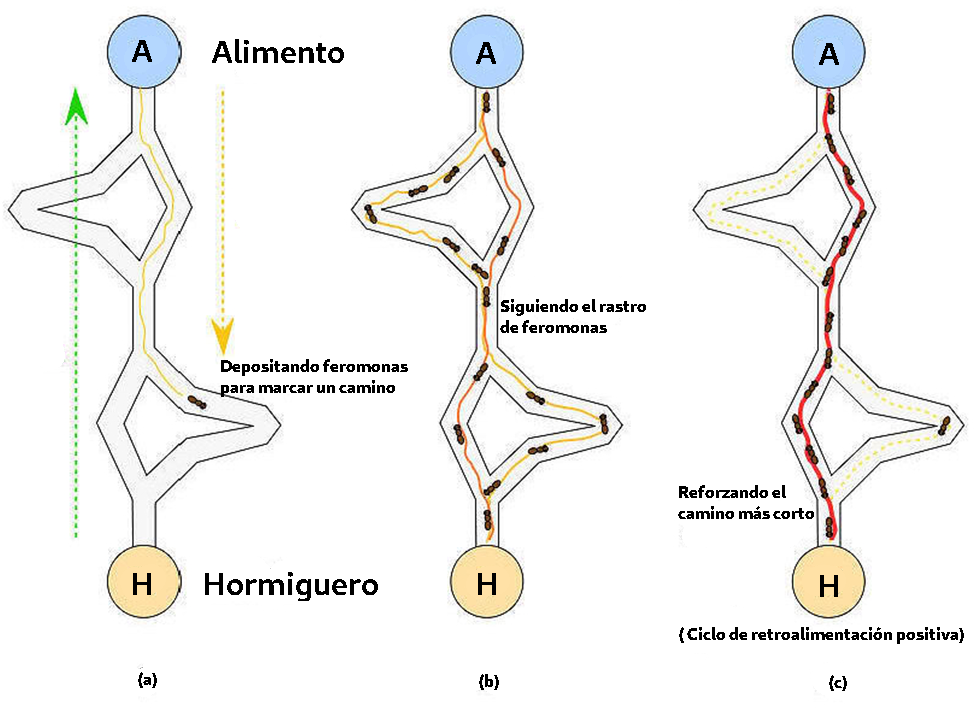
\includegraphics[scale=0.5]{imagenes/ACO-ant.png}
    \caption[Etapas de b\'usqueda de alimento y de comunicaci\'on entre hormigas.]{Etapas de b\'usqueda de alimento y de comunicaci\'on entre hormigas. (a) Flecha verde refleja la direcci\'on de la  b\'usqueda aleatoria, mientras que la flecha amarilla indica como una hormiga va depositando feromonas. (b) Otras hormigas siguen rastros de feromonas existente, aportando con sus propias feromonas. (c) Convergencia de las hormigas sobre el camino m\'as corto en base a la cantidad de feromonas depositada por m\'ultiples hormigas mediante un ciclo de retroalimentaci\'on positiva. Fuente: \cite{liu2020improving}.}
    \label{fig:hormigas}
\end{figure}
%Imagen de un recorrido

El conjunto de caminos que recorren las hormigas, para ir del hormiguero hacia la fuente de alimento y de retorno, puede ser interpretado como un grafo que representa esta red de caminos. En esta representaci\'on, la b\'usqueda de caminos corresponde a encontrar conjuntos de nodos o aristas adyacentes, y una componente de soluci\'on $c_{i}$ corresponde a una arista, siendo el recorrido desde una arista inicial hasta una arista final. La construcci\'on de una soluci\'on utiliza hormigas artificiales, tambi\'en llamadas agentes, que se desplazan a trav\'es del grafo mediante aristas adyacentes. La elecci\'on de aristas en cada paso de la construcci\'on utiliza la informaci\'on de las feromonas de cada una de las aristas candidatas, formando la soluci\'on incrementalmente. La metaheur\'istica ACO, indicada en el Algoritmo \ref{ACO-Algo}, consiste en 4 etapas, donde las 3 \'ultimas no tienen un orden espec\'ifico.

\begin{algorithm}[H]
\SetAlgoLined
 Ajuste de Par\'ametros \& inicializaci\'on de feromonas\;
 \While{Criterio de finalización no se cumple}{
   Construcci\'on\_de\_soluci\'on\_de\_cada\_hormiga()\;
   M\'etodo\_de\_b\'usqueda\_no\_local(); //Paso opcional\\
   Actualizaci\'on\_de\_feromonas()\;
 }
 \caption{Algoritmo metaheur\'istica ACO}\label{ACO-Algo}
\end{algorithm}


%%% CAMI VA AQUI

\subsection{Soluci\'on de un modelo COP mediante la metaheur\'istica ACO}

Un problema de optimización con restricciones, (COP, Constrained Optimization Problem) puede ser representado como $P = (S, \Omega, F)$, donde S es el espacio de soluciones, $\Omega$ son las restricciones, y $F$ es la funci\'on objetivo. S esta definido por un conjunto discreto de variables $X = 1 \dotsc n$, con valores $v_{i}^{j} \in D_{i} = \{v_{i}^{1} \dotsc  v_{i}^{|D_{i}|}\}$. Se define como una variable {\it instanciada} la asignaci\'on a $X_i$ de un valor $v_{i}^{j} \in D_i$. Una solución candidata $s \in S$ es una soluci\'on factible si satisface las restricciones del conjunto $\Omega$. La funci\'on objetivo $F: S\rightarrow \mathbb R_{0}^{+}$, es la funci\'on de evaluaci\'on que asigna una puntuaci\'on a las soluciones candidatas. Al mismo tiempo, se define $s^{*}$ como una soluci\'on \'optima y $S^{*}$ como el conjunto que engloba todas las soluciones \'optimas, dado que pueden existir m\'ultiples soluciones $s^{*}$, y se relacionan mediante $s^{*} \in S^{*} \subseteq S $ \cite{socha2008ant}.
%Esta definici\'on permite aplicar la metaheur\'istica de optimizaci\'on basada en colonia de hormigas (ACO por su sigla en ingl\'es) a un modelo de un {\it COP}.
%COP es un CSP con función objetivo: https://en.wikipedia.org/wiki/Constrained_optimization#Constraint_optimization_problems

Es posible adaptar la definici\'on del modelo COP al modelo de feromonas de la metaheur\'istica ACO, mediante la asociaci\'on entre la definici\'on de variable {\it instanciada} del modelo COP y lo que representa un componente de soluci\'on o arista en un recorrido de una hormiga. 
Espec\'ificamente, si se extiende la definici\'on de componente de soluci\'on $c_{i}$ para que esta pueda tener valores $v_{i}^{j}$ que var\'ien dependiendo de un dominio $D_i$, el componente de soluci\'on pasa a ser $c_{ij}$. As\'i se obtiene la equivalencia entre la asignaci\'on $X_i = v_{i}^{j}$ que representa una variable {\it instanciada} del modelo COP, y la selecci\'on de un componente de soluci\'on $c_{ij}$,  para una soluci\'on o camino $s$ en ACO\cite{socha2008ant}.
%equivalente a una arista en esta investigaci\'on,


Luego, la definici\'on de una soluci\'on $s$ puede representarse como un conjunto de componentes de soluci\'on $c_{ij} \in C, i = 1 \dotsc n, j = 1 \dotsc |D_i|$. A su vez, la feromona asociada a una componente de soluci\'on se transforma de $\tau_i$ a $\tau_{ij}$. El Algoritmo  \ref{ACO-Algo} se modifica para representar la equivalencia entre el modelo COP y la metaheur\'istica ACO, a\~nadiendose las definiciones de los datos y el resultado esperado, quedando como lo indica el algoritmo \ref{COP-ACO-Algo}. 


\begin{algorithm}[H]
\SetAlgoLined
\KwData{Variables $X_i \dotsc X_n$, dominios $D_1 \dotsc D_n$, Restricciones $\in \Omega$}
\KwResult{conjunto s\textquotesingle $ \subseteq S$ != $\emptyset$, si existen soluciones factibles}
 Ajuste de Par\'ametros \& inicializaci\'on de feromonas \;
 \While{Criterio de finalización no se cumple}{
   Construcci\'on\_de\_soluci\'on\_de\_cada\_hormiga()\;
   M\'etodo\_de\_b\'usqueda\_no\_local(); //Paso opcional\\
   Actualizaci\'on\_de\_feromonas()\;
 }
 \caption{Algoritmo de un modelo COP adaptado a una metaheur\'istica ACO}\label{COP-ACO-Algo}
\end{algorithm}
%%\chapter{Problem\'atica de la Individualizaci\'on de Filamentos a partir de un Grafo}
\chapter{Antecedentes}
\label{chap:cap2}

%problema previo, o problema 0 que consiste en la generaci\'on de un grafo a partir de una imagen que contenga una red, que en este caso, representaria a una red de filamentos. 

En base lo expuesto en el cap\'itulo \ref{chap:stateoftheart}, para el enfoque de utilizar grafos para la individualizaci\'on de filamentos existe una brecha entre la obtenci\'on del grafo y su an\'alisis. Este paso previo, la extracci\'on de un grafo a partir de una imagen, lo denominamos como el problema previo o problema 0 y consiste en extraer un grafo $G = (V,E)$ de una imagen tal que $G$ sea un grafo simple, no dirigido, ponderado, conectado o desconectado, con o sin ciclos. Esto implica que exista a lo m\'as 1 arista por cada par de nodos adyacentes, prohibi\'endose la existencia de nodos conectados consigo mismos. Se definen los v\'ertices/nodos del grafo $G$ como $V(G)$ y las aristas de $G$ como $E(G)$. 
Que el grafo $G$ sea ponderado implica que para las aristas del grafo ($E(G)$), existen caracter\'isticas asociadas que se expresan como caracter\'isticas geom\'etricas, topol\'ogicas, espaciales y/u otras. Es importante evitar que $G$ sea un grafo completo, dado que con n nodos/v\'ertices $G$ llega a tener $\frac{n(n-1)}{2}$ aristas.
%$\forall e \in \quad E(G) \quad  \exists $ 

Algunas de las dificultades involucradas en la extracci\'on de informaci\'on a partir de una imagen se encuentran en los m\'etodos presentados en el cap\'itulo \ref{chap:stateoftheart}, dentro de las que destacan el ruido y la resoluci\'on. Un ejemplo de aquello se observa en la figura \ref{fig:NoConsenso}.

\begin{figure*}[h]
    \begin{tabular}{c c c}
        \multirow[c]{2}{*}[2.5cm]{
        \begin{subfigure}[t]{0.4\textwidth}
        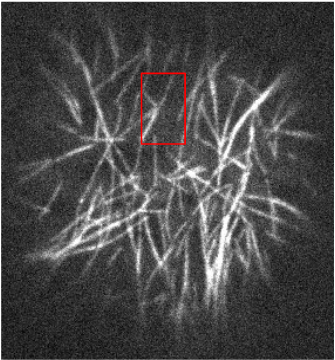
\includegraphics[scale=0.5]{imagenes/NoConsenso.png}
        \caption{Microt\'ubulos en planta {\it Marchantia}.\\Fuente: Paula Llanos}
        \label{fig:NoConsensoGeneral}
        \end{subfigure}  
        }
        &
        \multirow[c]{2}{*}[2cm]{
        \begin{subfigure}[t]{0.25\textwidth}
        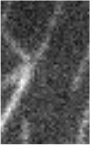
\includegraphics[]{imagenes/NoConsenso2.png}
        \caption{Secci\'on resaltada en rojo de \ref{fig:NoConsensoGeneral}}
        \label{fig:NoConsensoRect}
        \end{subfigure}
        }
        &
        \begin{subfigure}[t]{0.21\textwidth}
        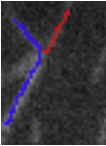
\includegraphics[scale=0.8]{imagenes/NoConsenso3.png}
        \caption{Opci\'on 1 de microt\'ubulos en \ref{fig:NoConsensoRect}}
        \label{fig:NoConsensoOpcion1}
        \end{subfigure} \\
        & &
        \begin{subfigure}[b]{0.21\textwidth}
        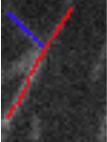
\includegraphics[scale=0.8]{imagenes/NoConsenso4.png}
        \caption{Opci\'on 2 de microt\'ubulos en \ref{fig:NoConsensoRect}}
        \label{fig:NoConsensoOpcion2}
        \end{subfigure} \\
    \end{tabular}
    
    \caption{Dificultad de individualizaci\'on que enfretan los expertos al analizar manualmente una imagen de filamentos, en particular, microt\'ubulos.}
    \label{fig:NoConsenso}
\end{figure*}

Mientras que el ruido ha sido estudiado en la literatura, el problema de resoluci\'on de filamentos depende principalmente de la capacidad del microscopio que se utilice. Como se menciona en la introducci\'on, el l\'imite m\'aximo de resoluci\'on, denominado $\frac{\lambda}{2}$, determina el tama\~no m\'inimo que 2 objetos que se encuentren juntos pueden tener para no observarse como un \'unico elemento. Lo anterior sucede para algunos tipos de filamentos como los microt\'ubulos que pueden medir tan solo 25 nan\'ometros, lo que se encuentra por debajo de $\frac{\lambda}{2}$ para diversos microscopios. 



Una vez obtenido el grafo que representa una red de filamentos, el problema siguiente se encuentra en el que 2 expertos pueden discernir con respecto a los filamentos identificables en una imagen, por lo que no es posible conocer a priori del origen y el final de un filamento, para las resoluciones actuales de las imagenes obtenidas a partir de la microscop\'ia. Se añade como dificultad que dada la representaci\'on de un filamento en un grafo se basa en un conjuntos de aristas adyacentes (denominadas caminos), pudiendo significar la b\'usqueda en un universo de hasta $n!$ posibles combinaciones.

A partir del problema anterior, el problema final en la individualizaci\'on de filamentos lo constituye la elecci\'on del subconjunto de caminos, que debe ser seleccionado entre el total de caminos que representan soluciones factibles. Esto implica que el problema no solo sea un problema combinatorial de generar soluciones factibles a partir del conjunto de aristas, sino que adem\'as debe considerar la discriminaci\'on entre estos para obtener el subconjunto de mayor calidad, pudiendo representarse como un problema de optimizaci\'on combinatorial.

Los 3 problemas presentados se formalizan a continuaci\'on.

%problema previo
%presentar el problema previo, como un puente necesario en la automatizaci\'on de la extracci\'on,  para analizar un grafo que representa la red de filamentos, que de lo contrario tendria que ser realizado a mano, implicando que la persona realizando el análisis podría llevar a cabo la individualizaci\'on de filamentos en el mismo acto.

\section{Generaci\'on de un Grafo desde una Imagen}
La extraci\'on o generaci\'on de un grafo que representa una red de filamentos a partir de una imagen es uno de las formas que define la cantidad de informaci\'on disponible para llevar a cabo la individualizaci\'on de filamentos. La importancia de este procedimiento radica en que a partir de la imagen es posible obtener una cantidad de caracter\'isticas de distinta \'indole, lo que permite en etapas posteriores clasificar de diversas formas nodos, aristas, de forma aislada o en conjuntos, efectivamente disminuyendo el espacio de b\'usqueda. Con las herramientas actuales disponibles en la literatura, es posible realizar la extracci\'on de una red de filamentos con algún nivel de informaci\'on como en \cite{xu2015soax}. Sin embargo, las transformaci\'on de aquella red a un grafo, as\'i como la incorporaci\'on de las caracter\'isticas y/o propiedades hacia el grafo son un procedimiento no automatizado, por lo que el esfuerzo que el experto debe realizar es cercano a individualizar los filamentos de manera manual.

A partir de las investigaciones en la literatura, es posible agrupar los m\'etodos para extraer la informaci\'on que permite la construcci\'on de un grafo a partir de una imagen, como lo son los nodos y las aristas, en dos conjuntos: Los que se basan en esqueletonizaci\'on\cite{lavado2018comparacion} y los que no. 

\subsection{Extracci\'on de un Grafo mediante Esqueletonizaci\'on}
\label{subsec:infoLossSkel}

%Que es la skeletonizacion y como extrae el grafo. Uso de liberia sknw
Los m\'etodos basados en esqueletonizaci\'on consisten primariamente en la reducci\'on de los p\'ixeles pertenecientes al plano de inter\'es o {\it foreground} en una imagen binaria, hasta formar una representaci\'on del objeto en la imagen de 1 p\'ixel de ancho. El proceso debe mantener la conectividad del objeto adelgazado y a su vez, reducir la dimensi\'on del objeto en la imagen para facilitar su an\'alisis\cite{saha2017skeletonization}. Un an\'alisis de los vecindarios de los p\'ixeles del esqueleto construido es una de las formas m\'as sencillas en que se puede distinguir si un p\'ixel representa un nodo o si es parte de un arista. Una librer\'ia que realiza tal an\'alisis es {\it skan}\cite{nunez2018new}, entregando estad\'isticas del grafo extra\'ido como largo promedio de una rama del esqueleto (equivalente a una arista del grafo), tipo de rama, curvatura de una rama, entre otras mediciones. Sin embargo, el formato de salida del grafo para esta herramienta corresponde a {\it Compressed sparse row} o CSR, lo que causa que un an\'alisis de mayor profundidad o el paso del grafo a una herramienta de individualizaci\'on de filamentos necesite de una librer\'ia adicional. 


Otra herramienta que realiza un an\'alisis similar para obtener un grafo a partir de un esqueleto es {\it sknw}, parte del framework {\it ImagePy}\cite{wang2018imagepy}. La diferencia propuesta por {\it sknw} radica en que se integra con la librer\'ia {\it NetworkX}\cite{hagberg2008exploring}, utilizando la estructura de datos para grafos que esta \'ultima posee para elegir entre m\'ultiples formatos de salida. Aquello otorga flexibilidad en la integraci\'on de herramientas que utilizan como base el grafo para realizar an\'alisis posteriores, como es el caso de la individualizaci\'on de filamentos.

%problema de skeleton
Independiente de la herramienta usada para obtener la informaci\'on topol\'ogica de la c\'elula observada, el procedimiento de esqueletonizaci\'on puede sufrir de p\'erdida de informaci\'on, dado que mediante el adelgazamiento utilizado se rompe la relaci\'on entre los p\'ixeles que conforman el elemento que se adelgaza y los p\'ixeles que constituyen el esqueleto obtenido. La informaci\'on que relaciona los p\'ixeles vecinos a los p\'ixeles del esqueleto es relevante ya que puede reflejar informaci\'on geom\'etrica como ancho o puede ser \'util al obtener informaci\'on derivada mediante m\'etodos como {\it image moments}\cite{flusser2009moments}\cite{chaumette2004image}. En base a lo anterior, se desarrolla una herramienta que captura esta informaci\'on a partir de la imagen usada en el proceso de esqueletonizaci\'on. A su vez, con esta herramienta tambi\'en es posible construir un grafo de la red de filamentos, sin embargo, el resultado no es de alta calidad. El procedimiento consta de los siguientes pasos:
% explicar que el hecho de G completo mediante lo q la arista es al problema de identificación de filamentos
%presento el extractor aproximado de grafos, la noción de puntos cluster/superPixels/blobs y el centro de masa como representante, dado que se puede obtener de forma simple mediante los "image moments". Además, distintos niveles de image moments permiten obtener información adicional útil en la descripción del cluster.

\begin{enumerate}
    \item Se generan clusters, tambi\'en llamados {\it super pixels} mediante una agrupaci\'on en base a un kernel de tama\~no 3x3, que busca separar de forma local los pixels que corresponden a {\it background} y no aportan informaci\'on, con respecto a los que son parte de la c\'elula observada ({\it foreground}), siendo estos \'ultimos los que concentran el inter\'es para el an\'alisis. La creaci\'on de clusters permite establecer la primera informaci\'on de vecindarios.
    \item Cada cluster es representado por un nodo, ubicado en el centro de masa del {\it super pixel}. En conjunto con el centro de masa es posible obtener informaci\'on geom\'etrica mediante los {\it raw image moments}\cite{chaumette2004image} del cluster. En este punto tambi\'en se procede a realizar fusiones de clusters en base a 2 criterios: Aquellos clusters con un n\'umero de p\'ixeles inferior a un umbral definido por el par\'ametro {\it Max\_Thickness} y los clusters que s\'olo tengan 2 vecinos y se encuentren bajo un umbral de cercan\'ia definido por el par\'ametro {\it Connectivity\_Threshold}. El par\'ametro {\it Max\_Thickness} hace referencia al ancho promedio de un filamento en la imagen y es definido por el usuario, mientras que {\it Connectivity\_Threshold} es el resultado del m\'ultiplo entre {\it Max\_Thickness} y un factor que depende de la c\'elula observada, variando entre 0.4 y 0.5. Una de las ventajas de fusionar clusters bajo los criterios mencionados radica en identificar y eliminar ciclos triangulares entre vecinos, mejorando la informaci\'on de vecindarios, sirviendo como una heurística para limitar el n\'umero de nodos.
    
    %\item A partir de la informaci\'on de vecindario de los nodos definitivos obtenidos en el paso anterior, se generan aristas entre nodos vecinos. Se obtiene el largo e  informaci\'on angular para cada arista creada. %Esta \'ultima es utilizada m\'as adelante para definir puntos de partida de las hormigas.
\end{enumerate}

Para asociar la informaci\'on de los vecindarios creados mediante los clusters con la informaci\'on extra\'ida mediante la esqueletonizaci\'on, se realiza un procedimiento similar al del paso 2, donde los nodos que representan clusters son fusionados con los nodo del esqueleto. 
Utilizando la posici\'on del nodo del esqueleto como centro de una matrix de tama\~no 3x3, se obtienen los clusters a los que pertenecen estos p\'ixeles. los cuales son absorbidos por el nodo del esqueleto respectivo, formando un nuevo cluster. Este nuevo cluster reemplaza a los clusters absobidos, heredando los vecinos que estos ten\'ian, pero manteniendo la posici\'on del nodo del esqueleto.

%Se define como generador {\it aproximado} de grafos debido a que puede sufrir de peque\~nas desviaciones en la ubicaci\'on de los nodos y las aristas con respecto a lo que otras herramientas de esqueletonizaci\'on e identificaci\'on de intersecciones en conjunto pueden hacer en la misma tarea. Uno de los objetivos en la creaci\'on del generador {\it aproximado} de grafos se debe a que facilita el uso de im\'agenes encontradas en el estado del arte.

En el caso que no sea posible obtener grafo mediante la esqueletonizaci\'on de la imagen, esta herramienta considera un paso adicional al procedimiento de 2 pasos presentado previamente. El tercer paso consiste en generar aristas entre los nodos vecinos, en base a la informaci\'on de vecindario, obteniendo el largo e informaci\'on angular para cada arista creada. El grafo generado se denomina como un grafo aproximado, ya que puede presentar deformaciones.


\subsection{Obtenci\'on de Informaci\'on Adicional}

Para dar uso a la informaci\'on recuperada de acuerdo a lo expresado en la secci\'on \ref{subsec:infoLossSkel}, se analizaron diversos filtros \'utiles para describir estructuras alargadas, como {\it Gabor}, {\it Anistropic Diffusion} y Frangi para {\it Veselness}. El filtro Frangi para {\it Veselness}\cite{frangi1998multiscale}\cite{fu2018frangi}, cuantifica cuan alargada es una estructura ({\it veselness value}), en base a los eigenvectores y eigenvalores de la matriz Hessiana (ecuaci\'on \eqref{eq:HessianMat}) posterior a la aplicaci\'on de uno o varios filtros Gaussianos para suavizar una imagen. Este filtro es utilizado en la detecci\'on de estructuras alargadas como arterias y venas, pudiendo replicarse parcialmente mediante el an\'alisis de p\'ixeles con {\it image moments}\cite{flusser2009moments}. La posibilidad de replicar el filtro de Frangi, sin necesidad de configurar par\'ametros, es lo que llev\'o a elegirlo por sobre las otras opciones.

\begin{equation}
    \label{eq:HessianMat}
    H = \begin{bmatrix}
        H_{xx} & H_{xy} \\
        H_{xy} & H_{yy} 
        \end{bmatrix}
\end{equation}

Una respuesta de {\it veselness value} que denota una estructura alargada se obtiene si los 2 eigenvalores, $\lambda_1$ y $\lambda_2$ ($|\lambda_2| \geq |\lambda_1|$) satisfacen $|\lambda_1| \approx 0 $ y $|\lambda_2| \gg |\lambda_1|$. Los eigenvalores se obtienen mediante la ecuaci\'on \ref{eq:lambdaFrangi}.

\begin{equation}
    \label{eq:lambdaFrangi}
    \lambda_{1,2} = \dfrac{(H_{xx} + H_{yy}) \pm \sqrt{(H_{xx} - H_{yy})^{2} + 4\cdot H_{xy}^{2}     } }{2}
\end{equation}

Otra forma de obtener los valores de lambda de la ecuaci\'on \ref{eq:lambdaFrangi} es utilizando los {\it central image moments} o momentos centrales, que derivan de los {\it raw image moments} obtenidos en el segundo paso la herramienta para recuperar informaci\'on presentada en la secci\'on \ref{subsec:infoLossSkel}. Se define un {\it raw image moment} de orden $p+q$ para una imagen en la ecuaci\'on \eqref{eq:rawImageMoment}, donde $f(x,y)$ corresponde a la intensidad de la imagen en un punto (x,y). El {\it raw moment} $M_{00}$ refleja la "masa" de la imagen, correspondiendo al \'area o volumen si se trata de una imagen binaria. 

Para el c\'alculo de los momentos centrales se agregan los componentes del centroide, $\overline{x}$ e $\overline{y}$, basados en los {\it raw moments}, como indican las ecuaciones \eqref{eq:avgFromRawMomts} y \eqref{eq:centralImageMoment}.

\begin{subequations}
\begin{equation}
    \label{eq:rawImageMoment}
    M_{pq} = \sum\limits_{x} \sum\limits_{y} x^p \cdot y^q \cdot f(x,y)
\end{equation}
\begin{equation}
    \label{eq:avgFromRawMomts}
    \overline{x} = \frac{M_{10}}{M_{00}}, \quad
    \overline{y} = \frac{M_{01}}{M_{00}}
\end{equation}
\begin{equation}
    \label{eq:centralImageMoment}
    \mu_{pq} = \sum\limits_{x} \sum\limits_{y} (x - \overline{x})^{p} \cdot (y - \overline{y})^{q} \cdot f(x,y)
\end{equation}
\end{subequations}

As\'i, es posible construir una matriz de covarianza, equivalente a la matriz hessiana en la ecuaci\'on \eqref{eq:HessianMat}, utilizando los momentos centrales de segundo orden, $\mu_{20}$, $\mu_{02}$ y $\mu_{11}$ divididos por el momento central de orden cero $\mu_{00}$ (ecuaciones \eqref{eq:mu20}, \eqref{eq:mu02} y \eqref{eq:mu11}), obteniendo los eigenvalores mediante la ecuaci\'on \eqref{eq:lambdaMoments}.

\begin{subequations}
\begin{align}
    \mu_{20}^{\prime} &= \frac{\mu_{20}}{\mu_{00}} = \frac{M_{20}}{M_{00}} - \overline{x}^{2} \label{eq:mu20} \\
    \mu_{02}^{\prime} &= \frac{\mu_{02}}{\mu_{00}} = \frac{M_{02}}{M_{00}} - \overline{y}^{2} \label{eq:mu02} \\
    \mu_{11}^{\prime} &= \frac{\mu_{11}}{\mu_{00}} = \frac{M_{11}}{M_{00}} - \overline{x}\cdot\overline{y} \label{eq:mu11}
\end{align}

\begin{equation}
    \label{eq:covMatLambda}
    cov[f(x,y)] = \begin{bmatrix}
        \mu_{20}^{\prime} & \mu_{11}^{\prime} \\
        \mu_{11}^{\prime} & \mu_{02}^{\prime} 
        \end{bmatrix}
\end{equation}

\begin{equation}
    \label{eq:lambdaMoments}
    \lambda_{1,2} = \dfrac{(\mu_{20}^{\prime} + \mu_{02}^{\prime}) \pm \sqrt{(\mu_{20}^{\prime} - \mu_{02}^{\prime})^{2} + 4\cdot \mu\prime_{11}^{2} }}{2}
\end{equation}
\end{subequations}

Con los valores de $\lambda$, es posible calcular caracter\'isticas de una estructura alargada como su excentricidad o su eje principal de inercia. Estas medidas pueden ayudar a mejorar la clasificaci\'on de segmentos del grafo durante la identificaci\'on de filamentos.


% informacion geometrica mediante calculo de angulos entre aristas
Un manera adicional de generar informaci\'on que facilite la discriminaci\'on de secciones del grafo es a trav\'es del c\'alculo de los \'angulos entre las aristas del grafo. Esto se relaciona a la propiedad de rigidez que tienen los filamentos, la que var\'ia dependiendo de la c\'elula en la que se encuentre el filamento, pudiendo delimitar la agrupaci\'on de aristas. Finalmente, para el caso de los nodos, el an\'alisis del grado de cada uno permite identificar la existencia de ciclos\cite{wilson1979introduction} en un filamento. La propiedad de un filamento de poder o no tener un ciclo es informaci\'on disponible priori que depende del tipo de c\'elula observada, permitiendo limitar posibles asociaciones entre nodos.


%se destaca dentro de los criterios: busca evitar perder información de la imagen/ampliar la informacion así como tener un costo computacional bajo, en conjunto con disminuir la interacción del usuario. 


% ambas opciones generan degeneraciones/deformaciones q afectan
\section{Exploraci\'on del Espacio de Soluciones}
definir que los segmentos/caminos/path son conjuntos de aristas adyacentes conectadas, o de nodos ..., que cumplen con restricciones, como la restricción angular o restricciones de ciclos (formula matem\'atica) y que los filamento son elegidos entre los caminos de mayor calidad
Un camino simple es equivalente a un \'arbol simple, ac\'clico...


%Un grafo completamente conectado puede tener n(n-1)/2 aristas, lo que para un n muy grande puede implicar un costo computacional alto
%A su vez, otro motivo para evitar que $G$ sea un grafo completo radica en que para los filamentos observados en la naturaleza no es una condici\'on comun... no encuentro la fuente de esto
En un grafo con n aristas, en el cual se desconoce el origen y el final los caminos, el n\'umero de combinaciones crece exponencialmente (agregar \cite{buchin2007number}\cite{biswas2012hamiltonian}). Denominamos todas estas opciones de caminos como el conjunto $P$, del cual debemos extraer un subconjunto $P'$ mediante una estrategia que permita realizar esto en tiempo polinomial independientemente de la cantidad de aristas del grafo.

\begin{equation}
p = (e_1, e_2,..., e_n)\\
p = ((v_1,v_2), (v_2,v_4),..., (v_n-1,v_n))
\label{eq:path}
\end{equation}

% explicar define
El m\'etodo presentado en \cite{breuer2015define} se basa en lo definido por \cite{lin2006vertex}, indicando que dado un problema de {\it covering}, existe un {\it set system}$(S,C)$, donde S es el conjunto total y finito de sets, y C es un conjunto de subsets pertenecientes a S. En el caso espec\'ifico del {\it Minimum Set Cover}(SC), el objetivo es encontrar un subconjunto $C'$ de $C$ tal que cada elemento de $S$ pertenezca al menos 1 vez a uno de los miembros de $C'$.

Para un {\it set system}$(S,C)$ que pueda ser representando por un \'arbol $T$, es posible modificar la definici\'on de $S$ al conjunto de nodos que componen un grafo $G$ y que cada subset $c \in C$ representa un camino\eqref{eq:path} simple en $G$. Se destaca que no necesariamente estar\'an todos los caminos simples de $G$ est\'an representados en $C$. Esta representaci\'on de {\it covering} de caminos, o {\it Path Cover}, es denominada {\it Vertex Covering by Paths on Graphs}(VcpG) y difiere de un {\it Path Cover} tradicional al permitir caminos que compartan nodos. Luego, para el caso de \'arboles, VcpG se renombra a VcpT ({\it Vertex Covering by Paths on Trees}), y si se reemplazan los nodos por aristas, lo no genera cambios significativos en el planteamiento del problema, se denomina EcpT {\it Edge Covering by Paths on Trees}. %recordar mas adelante como posible perdida de soluciones factibles


Lo anterior establece las bases para que los autores de DeFiNe\cite{breuer2015define} utilicen EcpT como base, teniendo un m\'aximo de caminos $n(n)-1/2 = \mathcal{O}(n^{2})$, con una complejidad $\mathcal{O}(n^{4})$ para obtener esos caminos, para caminos que no comparten nodos o aristas, es decir, no se sobrelapan.

La obtenci\'on de caminos a partir de un \'arbol $T$ que representa un grafo $G$ se realiza mediante la divisi\'on continua del \'arbol en m\'ultiples bosques, hasta que los bosques resultantes sean s\'olo caminos simples.

%aca entran las formas de obtener esos arboles simples y bosques, con las heuristicas de define
...


% Comparándose con define,
el problema acá está en la generación de P' subconjunto de P (caminos totales) , ya que al usar una sola propiedad, como lo puede ser el ángulo entre aristas, el largo o el ancho, se pierden soluciones. Ejemplo camino verde en Spinning Marchantia (imagenes)

% Heurística: hay alguna aca? pareciera solo satisfacci\'on de restricciones
% garantizar que al satisfacer las restricciones los caminos son solo soluciones factibles y que la unión de caminos también entrega múltiples opciones de filamentos, los que deben ser medidos para determinar cual es mejor




\section{Modelo de Optimización}
%dado que se tienen muchos filamentos, se debe evaluar cual es mejor. Explicar como propiedades topológicas y geométricas tienen. Y como se ponderan para un peso que será minimizado o maximizado

En base a lo recopilado en las secciones previas de esta investigaci\'on, es posible destacar los siguientes aspectos al problema a resolver:

\begin{itemize}
    \item Se desconoce a priori el n\'umero de filamentos a buscar, dado que una imagen puede tener individualizaciones distintas para 2 expertos.
    \item Generalmente, se busca individualizar m\'as de un filamento por imagen, lo que conlleva a elegir los mejores filamentos entre las soluciones que se encuentren.
    \item El uso de un grafo para representar la red de filamentos puede implicar que las combinaciones de soluciones crezcan de manera exponencial.
\end{itemize}

Lo anterior implica que el problema de identificar filamentos a partir de un grafo puede ser clasificado como un problema de optimizaci\'on de restricciones\cite{blum2011hybrid}.

Un problema de optimización de restricciones, (COP por su sigla en ingl\'es) puede ser representado como $P = (S, \Omega, F)$, donde S es el espacio de soluciones, definido por un conjunto discreto de variables $X = 1 \dotsc n$, con valores $v_{i}^{j} \in D_{i} = \{v_{i}^{1} \dotsc  v_{i}^{|D_{i}|}\}$. Se define como una variable {\it instanciada} la asignaci\'on a $X_i$ de un valor $v_{i}^{j} \in D_i$. Una solución candidata $s \in S$ es una soluci\'on factible si satisface las restricciones del set $\Omega$. La funci\'on objetivo $F: S\rightarrow \mathbb R_{0}^{+}$, es la funci\'on de evaluaci\'on que asigna valores a las soluciones candidatas. Al mismo tiempo, se define $s^{*}$ como una soluci\'on \'optima y $S^{*}$ como un conjunto de soluciones \'optimas, relacionados mediante $s^{*} \in S^{*} \subseteq S $\cite{socha2008ant}.
Esta definici\'on permite aplicar la metaheur\'istica de optimizaci\'on basada en colonia de hormigas (ACO por su sigla en ingl\'es) a un modelo de un {\it COP}.
%COP es un CSP con función objetivo: https://en.wikipedia.org/wiki/Constrained_optimization#Constraint_optimization_problems

\subsection{Metaheur\'istica ACO}
El proposito de la metaheur\'istica ACO es encontrar una soluci\'on o un set de soluciones. Una soluci\'on $s$ consiste en un conjunto de componentes de soluci\'on $c_{ij} \in C, i = 1 \dotsc n, j = 1 \dotsc |D_i|$, por lo que una concatenaci\'on de componentes de soluci\'on forma el camino o {\it tour} que recorre una hormiga, desde un nodo o arista inicial hasta un nodo o arista final. La metaheur\'istica ACO se muestra en el algoritmo \ref{ACO-Algo}. En base a la definici\'on de variable {\it instanciada} del modelo COP, se tiene que la asignaci\'on $X_i = v_{i}^{j}$ es equivalente a seleccionar un componente $c_{ij}$ para una soluci\'on $s$ en ACO.

ACO consiste en un paso de inicializaci\'on y de tres componentes, las que no tienen un orden espec\'ifico: {\it Construccion\_de\_soluci\'on\_de\_cada\_hormiga(),  M\'etodo\_de\_b\'usqueda\_no\_local()} y {\it Actualizaci\'on\_de\_feromonas()}.


\begin{algorithm}[H]
\SetAlgoLined
\KwData{Variables $X_i \dotsc X_n$, dominios $D_1 \dotsc D_n$, Restricciones $\in \Omega$}
\KwResult{conjunto s\textquotesingle $ \subseteq S$ != $\emptyset$, si existen soluciones factibles}
 Ajuste de Par\'ametros \& inicializaci\'on de feromonas \;
 \While{Criterio de finalización no se cumple}{
   Planificaci\'on\_de\_Pasos\;{
   ~ Construccion\_de\_soluci\'on\_de\_cada\_hormiga()\;
   ~ M\'etodo\_de\_b\'usqueda\_no\_local() \% opcional (DaemonActions)\;
   ~ Actualizaci\'on\_de\_feromonas()\;
   }Fin\_Planificaci\'on\_de\_Pasos\;
 }
 \caption{Algoritmo Metaheur\'istica ACO}\label{ACO-Algo}
\end{algorithm}


\subsubsection{M\'etodo Construccion de soluci\'on de cada hormiga}
La elecci\'on de un componente $c_{ij}$ por una hormiga durante la construcci\'on de un camino,
se lleva a cabo mediante el c\'alculo de una probabilidad para cada componente $c_{ij}$ posible de elegir. Este conjunto de vecinos factibles se denomina $N(s^{P}) \subseteq C$. En la probabilidad de selecci\'on influye el camino ya escogido, denominado soluci\'on parcial $s^{P}$. Al comenzar un recorrido, cada hormiga es asignada una arista de acuerdo a la heur\'istica de asignaci\'on, la cual analiza 3 situaciones:
\begin{enumerate}
\item La arista a asignar debe tener al menos uno de sus nodos con grado 1, indicando que es el inicio o final de una parte del grafo.

\item De no haber aristas con esas caracter\'isticas disponibles, se realiza una asignaci\'on inicial de una arista con uno de sus nodos con grado 2 o superior, siempre que uno de los nodos sea la uni\'on de esta arista con otra con la que conformen un \'angulo en el rango $]\theta, Max\_Angle]$. $\theta$ es un umbral que define el \'angulo m\'aximo, en grados, bajo el que se considera que 2 aristas contiguas respetan la rectitud necesaria para formar parte del mismo filamento. $Max\_Angle$ es un umbral que define el \'angulo m\'aximo, en grados, por sobre el cual se descarta de forma absoluta que 2 aristas contiguas forman parte del mismo filamentos. Este rango delimita los pares de aristas que a priori no representan combinaciones que respetan el criterio de rectitud, pero cuya explicaci\'on puede encontrarse en variaciones inducidas durante la extracci\'on del grafo desde la imagen, por lo que es necesario incorporar la exploraci\'on de estos pares de aristas.

\item De no existir aristas con alg\'un nodo que cumpla con los dos criterios previos, es posible asignar una arista aleatoria siempre que esta no forme parte de un camino recorrido por otra hormiga que haya sido evaluado como de buena calidad.
\end{enumerate}

% a diferencia de otros ACO, aca s^P != \emptyset al comienzo
Una vez asignada la primera arista seg\'un la heur\'istica previamente descrita, cada hormiga debe avanzar mediante la elecci\'on de nuevas aristas para a\~nadirlas a su recorrido. Este procedimiento se describe en la ecuaci\'on \eqref{eq:antProbabilities}, que corresponde a la probabilidad de elegir una arista a partir de un conjunto de aristas vecinas (conjunto $N(s^{P})$) dadas la aristas que ya pertenecen a la soluci\'on parcial de la hormiga ($s^P$), mediante la heur\'istica miope (ecuaci\'on \eqref{eq:heuristicaMiope}) que privilegia los candidatos que causen la menor desviaci\'on en la rectitud del camino. Se define que los componentes $c_{ij}$ que aportan con mayor probabilidad a la menor desviaci\'on son aquellos que en conjunto con el \'ultimo elemento elegido por la hormiga en ese punto ($c_{(i-1)j}$) forman un \'angulo en el rango $[0, \theta]$. El criterio de finalizaci\'on para la hormiga corresponde a que el conjunto $N(s^{P}) = \emptyset$.

%P(C_{ij} | s^{P}) = P_{n_{i},n_{j}} = P_{e_{x}}
\begin{equation}
P(c_{ij} | s^{P}) = \frac
        {\tau_{ij}^{\alpha} \cdot \eta_{ij}^{\beta}}
        {\sum\limits_{c_{ij}\in N(s^p)}{\tau_{ij}^{\alpha} \cdot \eta_{ij}^{\beta} } }, \forall c_{ij} \in N(s^{P})
\label{eq:antProbabilities}
\end{equation}

Otro aspecto de la ecuaci\'on \eqref{eq:heuristicaMiope} radica en la posibilidad de elecci\'on de elementos $c_{ij}$ que tienen un \'angulo en el rango $]\theta, \text{Max\_Angle}]$ con el componente de soluci\'on $c_{(i-1)j}$. Esto facilita la exploraci\'on de soluciones/caminos que de forma miope aparecen como de calidad no \'optima, y que para los efectos de este trabajo se denominan como de {\it calidad intermedia}. Esta evaluaci\'on consistente en disminuir la probabilidad de elecci\'on a medida que la diferencia entre el \'angulo que forman $c_{ij}$ y $c_{(i-1)j}$  , y la mitad de $\theta$ se incrementa.


%donde cada uno representa a una arista en esta investigaci\'on, y . Al momento de que la diferencia sea 90\textdegree, la probabilidad de asignaci\'on se reduce al 50\% de la probabilidad de un componente $c_{ij} \in [0, \theta]$.

\begin{equation}
    \eta_{ij} = 
        \begin{cases} 
        \text{Max\_Score si } \measuredangle(c_{ij}, c_{(i-1)j}) \in [0, \theta]\\[3ex]
        
        \text{Max\_Score} \cdot \left(1 - \dfrac{ \left| \measuredangle(c_{ij}, c_{(i-1)j}) - \frac{\theta}{2} \right|} {180} \right)  \text{ si } \measuredangle(c_{ij}, c_{(i-1)j}) \in \quad ]\theta, \text{Max\_Angle}].\\[3ex]
        
        \text{0 en otro caso;}
        \end{cases}
    \label{eq:heuristicaMiope}
\end{equation}

Con la finalidad de cuantificar la calidad de la soluci\'on construida por una hormiga, en cada selecci\'on de arista realizada, se suma el resultado de la heur\'istica miope al valor que la calidad de la hormiga lleva hasta ese punto. Cada hormiga comienza con una calidad 0, que al finalizar el {\it tour} es dividida por el n\'umero de aristas menos 1, para normalizar. Se establece que para ser considerada una soluci\'on de buena calidad, la hormiga debe tener una calidad mayor o igual a $\frac{Max\_Score}{2}$.
    
\subsubsection{M\'etodo de b\'usqueda no local}
Una vez que la hormiga termina un {\it tour}, es posible agregar un m\'etodo de {\it feedback} sobre la calidad del recorrido realizado, basado en l\'ogicas globales/centralizadas que escapan de la b\'usqueda local que realiza cada hormiga. Estos m\'etodos, denominados {\it Daemon Actions} en ingl\'es, permiten en el caso de una metaheur\'istica ACO gen\'erica seleccionar las hormigas de mejor calidad para incrementar las feromonas m\'as alla de lo que la {\it Actualizaci\'on\_de\_feromonas()} lo hace. 

Para la individualizaci\'on de filamentos, la evaluaci\'on global corresponde a eliminar soluciones candidatas que no aporten informaci\'on nueva. A modo de ejemplo, si $s_a$ y $s_b$ son las soluciones de las hormigas $a$ y $b$ respectivamente y cumplen con las siguientes condiciones:

\begin{itemize}
    \item $\forall c_{ij} \in s_a \in [0, \theta]$ y $\forall c_{ij} \in s_b \in [0, \theta]$
    \item $\forall c_{ij} \in s_a$ fueron electos por la hormiga $a$ con $P(c_{ij} | s_{a}^{P}) = 1$ y $\forall c_{ij} \in s_b$ fueron electos por la hormiga $b$ con $P(c_{ij} | s_{b}^{P}) = 1$
    \item $s_a \subseteq s_b$
\end{itemize}

Se tiene que $s_a$ no aporta m\'as informaci\'on que $s_b$, por lo que $s_a$ puede descartarse. Se denomina a $s_b$ como un segmento, el cual se comporta como una secci\'on indivisible de filamento. Este m\'etodo se ejecuta al comparar dos soluciones 
%RIESGO ASOCIADO a overmatch!!

%Si dos soluciones, $s_i$ y $s_j$ de las hormigas $i$,$j$, conformadas solamente por componentes $c_{ij} \in [0, \theta]$  (todos los componentes son de {\it buena calidad}), y que adem\'as eran la \'unica opci\'on posible en cada avance de la hormiga (probabilidad 1 de ser elegidas)
%tal que $s_i \subseteq s_j$ o viceversa, se tiene que una soluci\'on candidata no aporta nueva informaci\'on.
    
\subsubsection{M\'etodo Actualizaci\'on de feromonas}
\label{subsec:pheroUpdate}
Una vez que la hormiga termina un {\it tour}, esta debe actualizar las feromonas ($\tau_{ij}$) asociadas a los componentes de soluci\'on que la conforman. En una metaheur\'istica ACO tradicional, se aumenta el valor en los $c_{ij}$ que construyen un camino de buena calidad, mientras que debe realizar lo contrario para los componentes de soluci\'on que son parte de un recorrido de mala calidad. Adem\'as, los valores de las feromonas sufren decaimiento en el tiempo, dado por el par\'ametro $\rho$, que busca evitar la convergencia que las feromonas pueden causar en caminos de buena soluci\'on obtenidos al inicio de las iteraciones.


En la individualizaci\'on de filamentos, se utilizan {\it anti-feromonas}, con el proposito de indicar a las hormigas de futuras iteraciones cuales combinaciones de aristas/componentes de soluci\'n no llevan a resultados de buena calidad. Esto se fundamenta en la utilidad de las {\it anti-feromonas} para acotar el espacio de soluciones $S$. La forma de usar las {\it anti-feromonas} corresponde a {\it Substractive Anti-Pheromone} (SAP por su sigla en ingl\'es), la que introduce el par\'ametro $\gamma$ como factor de reducci\'on/penalizaci\'on. \cite{montgomery2002anti} indica que con $\gamma = 0.5$ SAP obtiene los mejores resultados. Por otra parte, el par\'ametro $\rho$ utilizado en las feromonas tradicionales no se utiliza en SAP.


Una modificaci\'on que se introduce en este trabajo con respecto a la aplicaci\'on de  feromonas y anti-feromonas es que estas com\'unmnente s\'olo se encuentran asociadas al componente $c_{ij}$ respectivo. Como variaci\'on para la individualizaci\'on/reconocimiento de filamentos, se propone asociar el valor de la anti-feromona no s\'olo con el componente $c_{ij}$, sino que adem\'as con uno o m\'as de los elementos que fueron elegidos en pasos anteriores por la hormiga que los selecciona. La explicaci\'on de lo anterior se basa en la posbilidad de desglosar una soluci\'on $s$ en segmentos $seg_{n}$ donde $n$ se\~nala el n\'umero de segmento al que corresponde dentro de la soluci\'on $s$. El segmento $seg_1$ comienza con la primera arista/componente $c_{ij}$ asignada a la hormiga de acuerdo a la heur\'istica de asignaci\'on, y termina en el primer elemento $c_{ij}$ con el que forma un \'angulo de calidad intermedia (sin incluirlo), siendo este mismo elemento el que inicia el segmento siguiente.
%Existen $N + 1$ segmentos en $s$ si la soluci\'on contiene $N$ elementos $c_{ij} \in ]\theta, 90]$ (de calidad intermedia). 


Luego, mediante la anti-feromona se relaciona un segmento $seg_n \subset s$ y la componente de soluci\'on $c_{ij} \in seg_{n+1} \in s$, cuya combinaci\'on es parte de una soluci\'on de mala calidad, con el fin de evitar que otras hormigas que pasen por $seg_n$ elijan $c_{ij}$. El rol de la anti-feromona es penalizar la probabilidad de elecci\'on de $c_{ij}$ para las hormigas que tengan al segmento $seg_n$ en su soluci\'on parcial $s^{P}$. Se debe destacar que esto es necesario ya que si s\'olo se utiliza la anti-feromona para penalizar $c_{ij}$, se puede ocasionar la perdida de capacidad de exploraci\'on de hormigas que provengan de otros recorridos parciales distintos a $seg_n$. La perdida de exploraci\'on tambi\'en sucede en el caso que el segmento $seg_{n+1}$ contenga solo 1 arista y no sea el segmento en el que finaliza el recorrido de la hormiga. Para subsanar aquel caso, a este tipo de segmentos se le a\~naden los nodos del segmento que lo precede, $seg_{n}$, con el objetivo de evitar que el an\'alisis del par $seg_{n+1}$ con la componente $c_{ij}$ que inicia el segmento $n+2$ sea s\'olo de 2 aristas.


Adicionalmente a lo anterior, se ha agregado un l\'imite de 2 penalizaciones como m\'aximo para cada anti-feromona. Al alcanzar este l\'imite, se reduce el valor de la anti-feromona a 0, haciendo imposible la elecci\'on de la componente de soluci\'on $c_{ij}$ para las hormigas cuya soluci\'on parcial $s^{P}$ contenga el segmento en el par componente,segmento penalizado.


La anti-feromona se aplica sobre hormigas que han finalizado su recorrido y cuya calidad normalizada sea menor a {\it Max\_Score}, ya que esto implica que al menos 1 de las aristas del recorrido es de calidad intermedia, necesitando un an\'alisis adicional para determinar si corresponde a una soluci\'on de buena calidad. El an\'alisis adicional consiste en evaluar la curvatura del recorrido, as\'i como la magnitud del desplazamiento entre la proyecci\'on de un segmento en relaci\'on a otro segmento contiguo. 

La curvatura de recorrido de una hormiga $a$ es el \'angulo formado por el nodo inicial ($n_{a1}$), el centro de masa de la misma hormiga ($mc_{a}$) y el nodo final ($n_{af}$). Este \'angulo no debe superar el umbral definido al multiplicar el \'angulo $\theta$ por un factor denominado {\it Max\_Axial\_Displacement}. Este factor permite flexibilizar la tolerancia de la curvatura en base a $\theta$. Si el recorrido de la hormiga tiene un \'angulo igual o mayor al umbral, implica que la soluci\'on encontrada es demasiado curva para representar un filamento, por lo que se penaliza el par $\langle c_{ij}$,$ seg_{n}\rangle$ donde $c_{ij}$ es la componente de soluci\'on/arista que inicia el \'ultimo segmento de la hormiga, mientras que $seg_{n}$ es el segmento que lo precede. Posterior a la penalizaci\'on, se desecha la soluci\'on.

El criterio de curvatura se refleja en la ecuaci\'on \eqref{eq:antiPheroSAP_Angle}.
%\begin{equation}
%    \label{eq:antiPheroSAP_Angle}
%    \tau_{ij} \leftarrow \tau_{ij} \cdot \gamma \quad \forall \langle c_{ij},seg_{n}\rangle > \textrm{Max\_Axial\_Displacement}
%\end{equation}

\begin{equation}
    \tau_{ij} \leftarrow
        \begin{cases}
        \tau_{ij} \cdot \gamma \text{ si } \measuredangle((n_{a1}, mc_{a}), (mc_{a}, n_{af})) < \theta \cdot \text{Max\_Axial\_Displacement}\\[3ex]
        
        \text{0 si } \tau_{ij} \leq 0.25 \\[3ex]
        \tau_{ij} \quad \text{en otro caso}
        \end{cases}
    \label{eq:antiPheroSAP_Angle}
\end{equation}

%agregar referencia? tindemans rod straightness \cite{hawkins2010model} of MTs o 
El an\'alisis respecto a la magnitud del desplazamiento entre la proyecci\'on de un segmento en relaci\'on a los segmentos que lo preceden se fundamenta en la rigidez que algunos tipos de filamentos, como los microt\'ubulos y los filamentos de actina poseen\cite{stam2017filament}. El criterio de rigidez consiste en analizar los segmentos con respecto a la totalidad de sus predecesores, comenzando por el \'ultimo segmento recorrido por la hormiga, es decir, desde el extremo final de la soluci\'on. A partir de cada par de segmento-predecesores, $\langle seg_{n}$,$seg_{1,n-1}\rangle$, se debe seleccionar el miembro del par de mayor longitud, definido como $s_{max} = \max(\norm{seg_{n}}, \norm{seg_{1,n-1}})$, para calcular el \'angulo suplementario que forma con respecto al otro miembro del par, definido como $s_{min}$. El \'angulo suplementario, $\measuredangle supl(s_{max},s_{min})$ es el equivalente a calcular el \'angulo entre la proyecci\'on de $s_{max}$ y $s_{min}$.

Luego $s_{min}$ es multiplicado por el seno del \'angulo suplementario, estableciendo el desplazamiento con respecto al eje que forma $s_{max}$ y su proyecci\'on. El umbral que delimita al desplazamiento calculado previamente se define como el m\'ultiplo de $s_{max}$ por 10\% de {\it Max\_Axial\_Displacement}. 

Si el \'angulo suplementario es menor a $\theta$, se puede declarar que se cumple el criterio de rigidez. Lo anterior se refleja en la ecuaci\'on \eqref{eq:antiPheroSAP_Axial}. 


%Esta propiedad puede ser utilizada para delimitar como un segmentos de una hormiga se relacionan con el resto de la soluci\'on, ya que estos ser\'ia un reflejo indirecto de los movimientos din\'amicos de un filamento en el tiempo, capturados en un punto a trav\'es de una imagen. 
%La rigidez de un filamento puede describirse mediante la relaci\'on que existe entre un segmento de una hormiga, con respecto a todos los segmentos que lo preceden. 
\begin{equation}
    \tau_{ij} \leftarrow
        \begin{cases}
        \begin{split}
         \tau_{ij} \cdot \gamma \text{ si } & \sin(\measuredangle supl(s_{max},s_{min}) > s_{min} \cdot 0.1 \cdot \text{Max\_Axial\_Displacement} \\ & \land \measuredangle supl(s_{max},s_{min}) > \theta    
        \end{split}
        \\[3ex]
        
        \text{0 si } \tau_{ij} \leq 0.25 \\[3ex]
        \tau_{ij} \quad \text{en otro caso}
        \end{cases}
    \label{eq:antiPheroSAP_Axial}
\end{equation}

Si ambas evaluaciones son completadas correctamente, se declara a la soluci\'on como de buena calidad.

%Finalmente, la ecuaci\'on \eqref{eq:antiPheroSAP} refleja la aplicaci\'on de las {\it anti-feromonas} sobre el par $\langle c_{ij}$,$ seg_{n}\rangle \forall c_{ij} \in ]\theta, Max\_Angle]$  donde $c_{ij} \in seg_{n+1}$, y cuya elecci\'on dio lugar a $seg_{n+1}$ que se aleja del desplazamiento axial m\'aximo que un filamento puede soportar.

En relaci\'on a los dominios $D_i$ declarados en la definici\'on del modelo de un COP, se destaca que en el caso de la individualizaci\'on de filamentos existe solo $D_1 \in D$, ya que la instanciaci\'on de variables ($X_i = v_{i}^{j}$ o $c_{ij}$) tiene una sola asignaci\'on posible, lo que lleva a una simplificaci\'on del componente $j$ en las ecuaciones presentadas.

\subsubsection{Inicializaci\'on de la metaheur\'istica ACO}

En el paso de inicializaci\'on de ACO se deben definir los valores de los par\'ametros relacionados a las feromonas y las heur\'isticas utilizadas. Para las feromonas se configura el valor inicial de $\tau_{ij}$ en 1 para los pares $\langle c_{ij}$,$ seg_{n}\rangle \> \forall c_{ij} \in \> ]\theta, Max\_Angle]$, dado que al usar SAP esta probabilidad se ir\'a reduciendo de acuerdo a un factor $\gamma$ seg\'un lo explicado en la secci\'on \ref{subsec:pheroUpdate}. El valor de $\gamma$ se define en 0.5, en base a lo encontrado en la literatura.

En el caso de los par\'ametros utilizados en diversas partes del modelo de optimizaci\'on, $\theta$ y {\it Max\_Axial\_Displacement} se encuentran asociados al tipo de c\'elula que se observa, lo que debe ser indicado como informaci\'on a priori. Los valores de $\theta$ son de 30\textdegree ~para microt\'ubulos de planta y neuronas. Por su parte, {\it Max\_Axial\_Displacement} recibe un valor de 1.5 para el caso de los microt\'ublos de planta o de 2.5 para las neuronas. Existen otras opciones de c\'elulas disponibles en la implementaci\'on del modelo de optimizaci\'on. El par\'ametro {\it Max\_Angle} se define como el m\'aximo entre 2.5 veces $\theta$ y 90. El par\'ametro {\it Max\_Score} utilizado por la heur\'istica miope se fija en 2.


Por su parte, el criterio de finalizaci\'on consiste en generar nuevas hormigas hasta que todas las aristas sean parte de al menos una soluci\'on de buena calidad, o que el n\'umero de hormigas generadas sea superior a 4 veces la cantidad de aristas.


En resumen, las condiciones del problema de identificaci\'on de filamentos dan pie a establecer su representaci\'on mediante un problema de optimizaci\'on de restricciones (COP), estando el modelo para la resoluci\'on del COP basado en la metaheur\'istica ACO para su resoluci\'on.
\chapter{Algoritmo Propuesto}
\label{sec:modeloOpti}
%dado que se tienen muchos filamentos, se debe evaluar cual es mejor. Explicar como propiedades topológicas y geométricas tienen. Y como se ponderan para un peso que será minimizado o maximizado

En base a lo recopilado en los cap\'itulos previos de esta investigaci\'on, es posible destacar los siguientes aspectos del problema a resolver:

\begin{itemize}
    \item Se desconoce a priori el n\'umero de filamentos a buscar.%, dado que una imagen puede tener individualizaciones distintas para 2 expertos.
    \item Generalmente se busca individualizar m\'as de un filamento por imagen, lo que conlleva a elegir los mejores filamentos entre las soluciones que se encuentren.
    \item El uso de un grafo para representar la red de filamentos puede implicar que las combinaciones de soluciones crezcan de manera exponencial.
\end{itemize}

Lo anterior permite clasificar el problema de identificar filamentos a partir de un grafo como un problema de optimizaci\'on con restricciones \cite{blum2011hybrid}.


%\section{Individualizaci\'on de filamentos mediante la metaheur\'istica ACO}
%similitud entre ambos
Se ha establecido en la secci\'on \ref{sec:OptiMethods} que una red de filamentos puede ser representada mediante un grafo, de forma similar a lo que sucede con la representaci\'on del conjunto de caminos que las hormigas recorren en b\'usqueda de alimento. En particular, un filamento en un grafo corresponde a un conjunto de aristas adyacentes, con lo que se puede asociar la individualizaci\'on de un filamento a la elecci\'on de una o m\'as aristas o componentes de soluci\'on, tal como se lleva a cabo en la metaheur\'istica ACO. A su vez, durante la elecci\'on de las aristas adyacentes que permiten individualizar un filamento, se puede utilizar una o m\'as caracter\'isticas que las aristas o componentes de soluci\'on poseen, para dirimir entre las aristas a elegir durante este proceso. Este comportamiento es similar al que las hormigas realizan utilizando las feromonas. Lo anterior constituye el fundamento para utilizar la metaheur\'istica ACO en el proceso de construcci\'on y evaluaci\'on de soluciones que permiten individualizar filamentos.

%Problema de explorar el espacio de soluciones
%comportamiento de las hormigas se puede asemejar a la forma en que los filamentos fueron creciendo o decreciendo.
La b\'usqueda de conjuntos de aristas adyacentes para individualizar uno o m\'as filamentos implica examinar un espacio de soluciones que no es posible de recorrer en tiempo polinomial, dado que sin restricciones las combinaciones crecen exponencialmente\cite{buchin2007number}\cite{biswas2012hamiltonian}. La metaheur\'istica ACO permite en sus distintas etapas (Construcci\'on de soluci\'on, b\'usqueda no local, actualizaci\'on de feromonas) incorporar informaci\'on que puede acotar el espacio de b\'usqueda. En el caso de la individualizaci\'on de filamentos, las diversas caracter\'isticas asociadas a las aristas, as\'i como las caracter\'isticas que definen el comportamiento global de un filamento permiten realizar esta tarea. 

%En relaci\'on a los dominios $D_i$ declarados en la definici\'on del modelo de un COP, se destaca que en el caso de la individualizaci\'on de filamentos existe solo $D_1 \in D$, ya que la instanciaci\'on de variables ($X_i = v_{i}^{j}$ o $c_{ij}$) tiene una sola asignaci\'on posible, lo que lleva a una simplificaci\'on del componente $j$ en las ecuaciones presentadas.

\section{Inicializaci\'on de la metaheur\'istica ACO}
\label{sec:acoInit}
En el paso de inicializaci\'on de ACO se deben definir los valores de los par\'ametros relacionados a las heur\'isticas y de las feromonas utilizadas. Una de las caracter\'isticas m\'as relevantes para discriminar aristas en el proceso de construcci\'on corresponde al \'angulo que forman 2 aristas adyacentes.
El primer umbral que permite definir si ambas aristas pertenecen al mismo filamento se define como $\theta$. As\'i, si el \'angulo se encuentra en el rango $[0, \theta]$ se puede dirimir que ambas aristas pertenecen al mismo filamento. Un segundo umbral se define como $Max\_Angle$, que indica el l\'imite por sobre el cual se puede inferir que estas 2 aristas no pertenecen al mismo filamento. Estos par\'ametros dependen de la c\'elula observada, asignando a $\theta$ valores de 30\textdegree ~para microt\'ubulos de planta y de 45\textdegree~ para neuronas. $Max\_Angle$ depende de $\theta$ al definirse como el m\'aximo entre 2.5 veces $\theta$ y 90\textdegree.

Otros par\'ametros a utilizar corresponden a {\it Max\_Axial\_Displacement} y a {\it Max\_Score}. El primero hace referencia a un par\'ametro de tolerancia que influye en 2 aspectos: al evaluar la curvatura general de una soluci\'on, y al evaluar la bifurcaci\'on entre 2 grupos de aristas al interior de la soluci\'on. La diferencia de la evaluaci\'on de bifurcaci\'on con respecto a la medici\'on de \'angulos entre aristas radica en que este criterio tambi\'en considera la magnitud de estos grupos de aristas. Los valores de {\it Max\_Axial\_Displacement} son de 1.5 para el caso de los microt\'ublos de planta o de 2.5 para las neuronas. Por su parte, {\it Max\_Score} define el puntaje m\'aximo a obtener por un camino de buena calidad. Su valor durante este trabajo corresponde a 2, y es utilizado por la heur\'istica miope (ecuaci\'on \ref{eq:heuristicaMiope}), que se define m\'as adelante en la secci\'on \ref{subsubsec:antTourInit}. A su vez, los par\'ametros $\alpha$ y $\beta$ tambi\'en utilizados en la heur\'istica miope, que regulan la ponderaci\'on entre esta heur\'istica y las feromonas, son fijados en 1.


En el caso de las feromonas, se define un valor inicial de $\tau_{ij} = 1$, pero utilizando un concepto inverso de feromona con respecto al que se present\'o previamente. El cambio consiste en el uso de {\it anti-feromonas} o SAP ({\it Substractive Anti-Pheromone})\cite{montgomery2002anti}, que se explica en la secci\'on \ref{subsec:pheroUpdate} y consiste en disminuir el valor de la feromona asociada a su respectiva arista. El uso de SAP introduce el par\'ametro $\gamma$, el que se define en 0.5 en base a lo encontrado en la literatura.

%%%%%%%%%%%%%%%%%%%%%%%%%%%%%%%%%%%%%%%%
%Para las feromonas se configura el valor inicial de $\tau_{ij}$ en 1 para los pares $\langle c_{ij}$,$ seg_{n}\rangle \> \forall c_{ij} \in \> ]\theta, Max\_Angle]$, dado que al usar SAP esta probabilidad se ir\'a reduciendo de acuerdo a un factor $\gamma$ seg\'un lo explicado en la secci\'on \ref{subsec:pheroUpdate}. El valor de $\gamma$ se define en 0.5, en base a lo encontrado en la literatura.
%%%%%%%%%%%%%%%%%%%%%%%%%%%%%%%%%%%%%

Finalmente, el criterio de finalizaci\'on consiste en generar nuevas hormigas artificiales hasta que todas las aristas sean parte de al menos una soluci\'on de buena calidad, o que el n\'umero de hormigas generadas sea superior a 4 veces la cantidad de aristas. En lo que sigue de este trabajo se utiliza el t\'ermino hormigas en referencia a las hormigas artificiales o agentes.


\section{M\'etodo de construccion de soluci\'on de cada hormiga}
\label{subsubsec:antTourInit}
Al comenzar un recorrido, cada hormiga es asignada una arista de acuerdo a la heur\'istica de asignaci\'on inicial, la que corresponde al primer elemento del camino o recorrido parcial $s^{P}$. La heur\'istica de asignaci\'on inicial analiza hasta 3 situaciones, dependiendo del tipo de c\'elula:
\begin{enumerate}
\item La arista a asignar debe tener al menos uno de sus nodos con grado 1, indicando que es el inicio o final de una parte del grafo.

\item De no haber aristas disponibles con esas caracter\'isticas, se realiza una asignaci\'on inicial de una arista que cumpla con 2 criterios:
\begin{itemize}
    \item Tener uno de sus nodos con grado 2 o superior.
    \item El \'angulo que forma la arista candidata a elegir, junto a otra arista a la que pertenece el nodo, debe pertenecer al rango $]\theta, Max\_Angle]$.
\end{itemize}
%$\theta$ es un umbral que define el \'angulo m\'aximo, en grados, bajo el que se considera que 2 aristas contiguas respetan la rectitud necesaria para formar parte del mismo filamento. $Max\_Angle$ es un umbral que define el \'angulo m\'aximo, en grados, por sobre el cual se descarta de forma absoluta que 2 aristas contiguas forman parte del mismo filamentos. Este rango delimita los pares de aristas que a priori no representan combinaciones que respetan el criterio de rectitud, pero cuya explicaci\'on puede encontrarse en variaciones inducidas durante la extracci\'on del grafo desde la imagen, por lo que es necesario incorporar la exploraci\'on de estos pares de aristas.

\item De no existir aristas con alg\'un nodo que cumpla con los dos criterios previos, es posible asignar una arista aleatoria. Esta arista no debe pertenecer al una soluci\'on o camino evaluado como de buena calidad. La calidad de un camino se presenta m\'as adelante en esta secci\'on.
\end{enumerate}

%a elecci\'on de un componente $c_{ij}$ por una hormiga durante la construcci\'on de un camino, se lleva a cabo mediante el c\'alculo de una probabilidad para cada componente $c_{ij}$ posible de elegir. Este conjunto de vecinos factibles se denomina $N(s^{P}) \subseteq C$. En la probabilidad de selecci\'on influye el camino ya escogido, denominado soluci\'on parcial $s^{P}$. 

% a diferencia de otros ACO, aca s^P != \emptyset al comienzo
Una vez asignada la primera arista seg\'un la heur\'istica previamente descrita, cada hormiga debe avanzar mediante la elecci\'on de nuevas aristas para a\~nadirlas a su recorrido. Este procedimiento corresponde a la probabilidad de elegir una arista o componente $c_{ij}$ a partir de un conjunto de aristas vecinas $N(s^{P})$. Las aristas que pertenecen a $N(s^{P})$ son s\'olo las aristas adyacentes a la \'ultima arista agregada a la soluci\'on parcial $s^P$ que son factibles de agregar a la soluci\'on parcial. La factibilidad de a\~nadir una arista de $N(s^{P})$ a $s^{P}$ corresponde a la probabilidad expresada en la ecuaci\'on \ref{eq:antProbabilities}. Esta probabilidad depende del valor de la feromona $\tau_{ij}$ asociada a la arista $c_{ij}$, as\'i como del valor de la heur\'istica miope $\eta_{ij}$ (ecuaci\'on \ref{eq:heuristicaMiope}) que eval\'ua el \'angulo formando entre la arista $c_{ij} \in N(s^{P})$ y la \'ultima arista agregada a $s^{P}$, que se define como $s_{n}^{P}$.


En particular, la heur\'istica miope $\eta_{ij}$ entrega una puntuaci\'on que disminuye a medida que el \'angulo mencionado aumenta, siendo el rango $[0, \theta]$ el que otorga la puntuaci\'on m\'axima de $Max\_Score$. Si el \'angulo es mayor a $Max\_Angle$ la puntuaci\'on corresponde a 0. Para el rango intermedio $]\theta, Max\_Angle]$, la puntuaci\'on depende de la diferencia entre el \'angulo formando entre la arista $c_{ij} \in N(s^{P})$ y $s_{n}^{P}$. Mientras m\'as aumenta esta diferencia, menor es la puntuaci\'on asignada.


%que tiene asociada. Otro aspecto que influye en la elecci\'on de una arista es la desviaci\'on que puede ocasionar si se a\~nade a $s^P$, con respecto a la rectitud del camino ya recorrido. Esta evaluaci\'on se refleja en el valor $\eta_{ij}$ asociado a la arista, que se calcula mediante la heur\'istica miope. 
%mediante la heur\'istica miope (ecuaci\'on \ref{eq:heuristicaMiope}) que privilegia los candidatos que causen la menor desviaci\'on en la rectitud del camino. 
%Se define que las aristas $c_{ij}$ que aportan con mayor probabilidad a la menor desviaci\'on son aquellos que en conjunto con el \'ultimo elemento elegido por la hormiga en ese punto ($c_{(i-1)j}$) forman un \'angulo en el rango $[0, \theta]$. El criterio de finalizaci\'on para la hormiga corresponde a que el conjunto $N(s^{P}) = \emptyset$, es decir, que no existan opciones de aristas para seleccionar.

%P(C_{ij} | s^{P}) = P_{n_{i},n_{j}} = P_{e_{x}}
\begin{equation}
P(c_{ij} | s^{P}) = \frac
        {\tau_{ij}^{\alpha} ~ \eta_{ij}^{\beta}}
        {\sum\limits_{c_{ij}\in N(s^p)}{\tau_{ij}^{\alpha} ~ \eta_{ij}^{\beta} } }, \forall c_{ij} \in N(s^{P}).
\label{eq:antProbabilities}
\end{equation}

La evaluaci\'on de \'angulos entre aristas adyacentes que pertenezcan al rango intermedio $]\theta, Max\_Angle]$ en la heur\'istica miope, facilita la exploraci\'on de soluciones o caminos que de forma miope no califican como soluciones candidatas factibles de representar un filamento, pero que tampoco pueden ser descartados completamente. En el caso que un camino tenga uno o m\'as pares de aristas adyacentes cuyo \'angulo pertenezca a este rango, se definir\'a el camino como de {\it calidad intermedia}.

%Otro aspecto de la ecuaci\'on \ref{eq:heuristicaMiope} radica en la posibilidad de elecci\'on de aristas $c_{ij}$ que tienen un \'angulo en el rango $]\theta, \text{Max\_Angle}]$ con el componente de soluci\'on $c_{(i-1)j}$. Esto facilita la exploraci\'on de soluciones/caminos que de forma miope aparecen como de calidad no \'optima, y que para los efectos de este trabajo se denominan como de {\it calidad intermedia}. Esta evaluaci\'on consistente en disminuir la probabilidad de elecci\'on a medida que se incrementa la diferencia entre el \'angulo que forman $c_{ij}$ y $c_{(i-1)j}$, y la mitad de $\theta$.
%donde cada uno representa a una arista en esta investigaci\'on, y . Al momento de que la diferencia sea 90\textdegree, la probabilidad de asignaci\'on se reduce al 50\% de la probabilidad de un componente $c_{ij} \in [0, \theta]$.

\begin{equation}
    \eta_{ij} = 
        \begin{cases} 
        \text{Max\_Score si } \measuredangle(c_{ij}, s_{n}^{P}) \in [0, \theta],\\[3ex]
        
        \text{Max\_Score} \cdot \left(1 - \dfrac{ \left| \measuredangle(c_{ij}, s_{n}^{P}) - \frac{\theta}{2} \right|} {180} \right)  \text{ si } \measuredangle(c_{ij}, s_{n}^{P}) \in \quad ]\theta, \text{Max\_Angle}],\\[3ex]
        
        \text{0 en otro caso.}
        \end{cases}
    \label{eq:heuristicaMiope}
\end{equation}

Con la finalidad de cuantificar la calidad de la soluci\'on construida por una hormiga, en cada selecci\'on de arista realizada, se suma el resultado de la heur\'istica miope $\eta_{ij}$ a la calidad del camino que la hormiga lleva hasta ese punto. Cada hormiga comienza con una calidad 0, que al finalizar su recorrido es dividida por el n\'umero de aristas menos 1, para normalizar el valor entre las distintas soluciones. Se establece que para ser consideradas como una soluci\'on de {\it buena calidad}, la hormiga debe tener una calidad mayor o igual a $Max\_Score/2$. Es importante destacar que la calidad de una soluci\'on puede variar en cada etapa de la metaheur\'istica ACO, pudiendo descartarse una soluci\'on en base a los criterios de cada m\'etodo. El desechar una soluci\'on implica ajustar su calidad a 0, lo que la clasifica como de {\it mala calidad}. Las hormigas que en cada elecci\'on de arista hayan elegido componentes $c_{ij}$ que formaban un \'angulo en en rango $[0, \theta]$ con $s_{n}^{P}$, son las que obtienen el m\'aximo puntaje de $Max\_Score$ al normalizarse, y se definen como de {\it calidad \'optima}. Los caminos clasificados como de {\it calidad intermedia} son inicialmente parte del grupo de soluciones de buena calidad.

%Un planteamiento similar a lo anterior es el {\it Path Cover Problem} o PCP, en el que se descompone un grafo dirigido en caminos con el objetivo de obtener un conjunto de caminos. Cada nodo o arista debe pertenecer exactamente a un camino y los caminos pueden comenzar o terminar en cualquier parte del grafo.

%Esta reducci\'on del espacio de b\'usqueda debe considerar no eliminar soluciones o caminos v\'alidos, como puede suceder con casos de cruce o solapamiento de filamentos, o la existencia de ciclos. 


%En el caso de la individualizaci\'on de filamentos, es necesario que la definici\'on del problema considere como v\'alidos caminos que representen los casos de filamentos con o sin ciclos, as\'i como superposici\'on y/o cruce. Lo anterior impide forzar la pertenencia de un nodo o arista a un s\'olo camino


\section{M\'etodo de actualizaci\'on de feromonas}
\label{subsec:pheroUpdate}
Una vez que la hormiga termina un recorrido, se eval\'ua su calidad para actualizar las feromonas $\tau_{ij}$ asociadas a los componentes de soluci\'on que lo conforman. As\'i, en una metaheur\'istica ACO tradicional, se aumenta el valor de $\tau_{ij}$ en cada $c_{ij}$ que es parte de un camino de buena calidad. Adicionalmente, los valores de las feromonas sufren decaimiento en el tiempo, dado por el par\'ametro $\rho$, que busca evitar la convergencia que las feromonas pueden causar en caminos de buena calidad obtenidos al inicio de las iteraciones.


En la individualizaci\'on de filamentos, se utilizan {\it anti-feromonas}, con el prop\'osito de indicar a las hormigas de futuras iteraciones los caminos que no son de buena calidad. La diferencia radica en que las anti-feromonas buscan acotar el espacio de soluciones $S$ sin necesariamente buscar la convergencia sobre un \'unico camino. Este cambio implica no utilizar el par\'ametro $\rho$, ya que no existe decaimiento en este uso de anti-feromonas, y reemplazarlo por el par\'ametro $\gamma$ como factor de reducci\'on/penalizaci\'on \cite{montgomery2002anti}. Al ser la penalizaci\'on un factor que se aplica sobre el valor de $\tau_{ij}$, la anti-feromona puede disminuir constantemente sin llegar a valer exactamente cero, por lo que se define un l\'imite de 2 penalizaciones como m\'aximo para cada anti-feromona. Al alcanzar este l\'imite, se reduce el valor de $\tau_{ij}$ a 0, haciendo imposible la elecci\'on de la arista $c_{ij}$ respectiva.
%para las hormigas cuya soluci\'on parcial $s^{P}$ contenga el segmento en el par $<$componente,segmento$>$ penalizado. 

Adem\'as de cambiar el uso de feromonas por el de anti-feromonas, se introduce una segunda modificaci\'on, relativa a las aristas a las que aplica la penalizaci\'on de las anti-feromonas. Un uso tradicional de anti-feromonas implica la disminuci\'on del valor de $\tau_{ij}$ para su respectiva arista $c_{ij}$, en caso de que se trate de un camino de mala calidad. 
Esto puede llevar a la p\'erdida de exploraci\'on de soluciones en la individualzaci\'on de filamentos, ya que una arista con un $\tau_{ij}$ penalizado por pertenecer a uno o m\'as caminos de mala calidad, puede bloquear otros caminos, dado que el valor de $\tau_{ij}$ no guarda relaci\'on con el conjunto de aristas que causa la penalizaci\'on. As\'i, las soluciones que pudiesen pasar por esa arista se ven limitadas.

 
%En aquel caso, la \'unica arista de $seg_{n+1}$ se transforma en un cuello de botella para la exploraci\'on debido a que penaliza de forma indiscriminada a todas las hormigas que pasen por ah\'i, independientemente del \'angulo que forme con otras aristas o componentes. Para subsanar aquel caso, a este tipo de segmentos se le a\~naden los nodos del segmento que lo precede, $seg_{n}$, con el objetivo de evitar que el an\'alisis del par $seg_{n+1}$ con la componente $c_{ij}$ que inicia el segmento $n+2$ sea s\'olo de 2 aristas.

En este trabajo se propone que la penalizaci\'on de $\tau_{ij}$ guarde relaci\'on con el conjunto de aristas en el camino $s$ que preceden a la arista $c_{ij}$. Se define a aquel conjunto de aristas como un segmento de un camino recorrido por la hormiga $a$, expresado como $seg_{n}^{a}$. Los segmentos se generan durante la construcci\'on de un recorrido, existiendo siempre al menos un segmento en cada camino. Dado que el \'angulo entre 2 aristas adyacentes es uno de los criterios utilizados durante la construcci\'on de un camino, el fin de un segmento puede suceder en 2 casos: si la \'ultima arista en el camino corresponde al final del recorrido, o si la arista $s_{n}^{P}$ (la \'ultima arista agregada a $s^P$) forma un \'angulo en el rango $]\theta, Max\_Angle]$ con la arista $c_{ij} \in N(s^P)$ a agregar a la soluci\'on parcial.

\begin{figure}[h!]
    \centering
    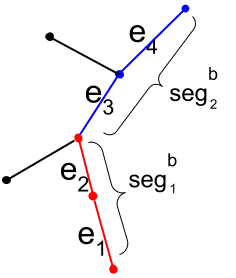
\includegraphics[scale=0.8]{imagenes/ant_segments_simple_case.png}
    \caption{Camino de una hormiga $b$ compuesto por 2 segmentos. El \'angulo entre las aristas $e_2$ y $e_3$ pertenece al rango $]\theta, Max\_Angle]$, finalizando el segmento $seg^{b}_1$ e iniciando el segmento $seg^{b}_2$. Fuente: Elaboraci\'on Propia.}
    \label{fig:segmentSimpleCase}
\end{figure}

As\'i, cada segmento esta formado por una o m\'as aristas, donde cada arista del segmento forma un \'angulo en el rango $[0, \theta]$ con sus vecinos. Un ejemplo de esto se puede observar en la Figura \ref{fig:segmentSimpleCase}, en el que si se penaliza la arista $e_3$, esta penalizaci\'on ser\'a asociada al segmento $seg^{b}_{1}$, disminuyendo la posibilidad de que futuras hormigas que recorran este segmento escojan $e_3$, sin perjuicio de otros caminos que pasen por $e_3$ pero no por el segmento $seg^{b}_{1}$.


Una ventaja de utilizar segmentos de camino es evitar volver a evaluar la relaci\'on entre todas las aristas que conforman el camino, ya que las aristas que conforman un segmento cumplen con un criterio para ser consideradas como parte del mismo filamento. As\'i, la evaluaci\'on de la calidad del camino se realiza s\'olo en el caso que 2 aristas vecinas formen un \'angulo de rango intermedio ($]\theta, Max\_Angle]$), enfoc\'andose en las soluciones de calidad intermedia que permiten explorar el espacio de soluciones.


Se debe se\~nalar que esta propuesta de penalizaci\'on realiza la evaluaci\'on de la calidad del camino en orden inverso al utilizado durante la construcci\'on del recorrido, imitando el retorno que realiza una hormiga desde el alimento hacia su hormiguero. Esto, sumando al uso de segmentos, permite comenzar la revisi\'on en el \'ultimo par de aristas cuyo \'angulo pertenece al rango intermedio, es decir, el nodo donde termina el pen\'ultimo segmento y comienza el \'ultimo. A modo de ejemplo, en la Figura \ref{fig:segmentSimpleCase}, esto ser\'ia el nodo com\'un de las aristas $e_2$ y $e_3$, que separa los segmentos $seg^{b}_1$ y $seg^{b}_2$. En este ejemplo, en caso de penalizar la arista $e_3$, ser\'a solo disminuyendo su posibilidad de ser elegida para caminos que contengan al segmento $seg^{b}_1$ en su soluci\'on.

%cortar de atras para adelante una sola vez permite acotar los caminos malos sin descartar una solucion completamente, solo sacando la parte potencialmente mala al final


Por \'ultimo en este aspecto, y a diferencia del uso tradicional de feromonas o anti-feromonas, donde se penalizan todas las aristas pertenecientes a una soluci\'on, el recorrido inverso y el uso de segmentos permite que sea suficiente la penalizaci\'on de una arista en la soluci\'on para clasificar la soluci\'on $s$ como de mala calidad y desecharla. Esto permite que a partir de una soluci\'on de mala calidad se remueva el \'ultimo segmento, permitiendo a otra hormiga recorrer un camino similar con un distinto final, favoreciendo la exploraci\'on. Para visualizar esto, es posible utilizar la Figura \ref{fig:segmentComplexCaseH}, en donde una hormiga pudiese construir un camino incorporando las aristas $e_1$, $e_2$, $e_4$, $e_5$ y $e_6$. Al desechar el \'ultimo segmento, conformado s\'olo por la arista $e_6$, permite que otra hormiga recorra desde $e_1$ hasta $e_5$, pudiendo agregar $e_7$ a su camino o terminando en $e_5$. 

\begin{figure}[h!]
    \centering
    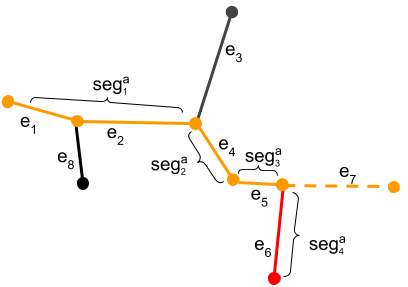
\includegraphics[scale=0.8]{imagenes/ant_segments_complex_case_H.png}
    \caption{Camino de una hormiga $a$ compuesto por 4 segmentos. El comienzo en orden inverso a la construcci\'on favorece la exploraci\'on, reemplazando el \'ultimo segmento por otro o simplemente concluyendo el recorrido. Fuente: Elaboraci\'on Propia.}
    \label{fig:segmentComplexCaseH}
\end{figure}

%Existen $N + 1$ segmentos en $s$ si la soluci\'on contiene $N$ elementos $c_{ij} \in ]\theta, 90]$ (de calidad intermedia). 
Lo anterior permite definir que la penalizaci\'on de $\tau_{ij}$ este asociada a la arista $c_{ij}$ y al segmento que precede a $c_{ij}$ en el recorrido de una hormiga $a$. El segmento que precede a $c_{ij}$ en un camino $s$ se define como $seg^{a}_{prev}$. Adicionalmente, se tiene que entre distintos caminos pueden existir segmentos equivalentes, lo que sucede en el caso de que contengan las mismas aristas. Esto permite que se refieran al mismo valor $\tau_{ij}$ a pesar de los nombres relativos al camino al que pertenecen. El funcionamiento del m\'etodo de penalizaci\'on propuesto se visualiza en la Figura \ref{fig:segmentComplexCase}.
 \begin{figure*}[t!]
    \centering
    \begin{subfigure}[t]{0.48\textwidth}
        \centering
        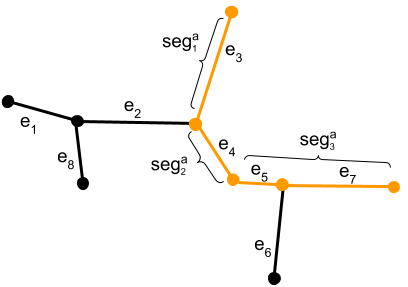
\includegraphics[height=2in]{imagenes/ant_segments_complex_case_1.png}
        \caption{Camino de una hormiga $a$ que contiene las aristas $e_3$, $e_4$, $e_5$ y $e_7$.}
        \label{fig:segmentComplexCase1}
    \end{subfigure}%
    ~ \hspace{0.5cm}
    \begin{subfigure}[t]{0.48\textwidth}
        \centering
        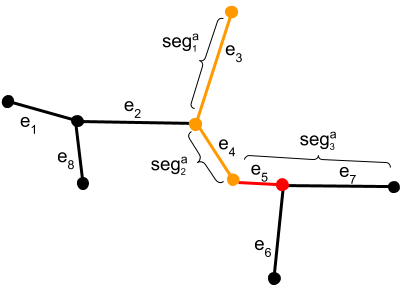
\includegraphics[height=2in]{imagenes/ant_segments_complex_case_2.png}
        \caption{Penalizaci\'on del camino de la hormiga $a$ en la arista $e_5$ con respecto al segmento $seg^{a}_2$ conformado solo por la arista $e_4$.}
        \label{fig:segmentComplexCase2}
    \end{subfigure}

\vskip\baselineskip
    \begin{subfigure}[t]{0.48\textwidth}
        \centering
        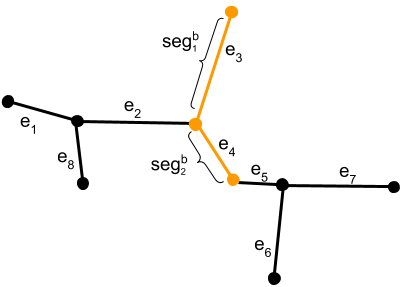
\includegraphics[height=2in]{imagenes/ant_segments_complex_case_4.png}
	    \caption{Camino de una hormiga $b$ que contiene las aristas $e_3$, $e_4$. El camino $b$ no puede agregar la arista $e_5$ debido a que se encuentra penalizada para el segmento formado por la arista $e_4$.}
        \label{fig:segmentComplexCase3}
    \end{subfigure}%
    ~ \hspace{0.5cm}
    \begin{subfigure}[t]{0.48\textwidth}
        \centering
        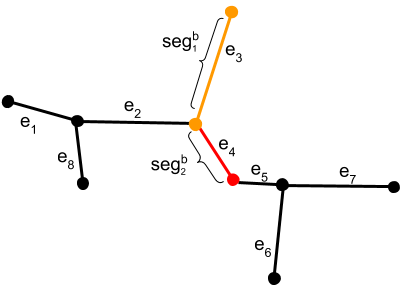
\includegraphics[height=2in]{imagenes/ant_segments_complex_case_5.png}
        \caption{Penalizaci\'on del camino de la hormiga $b$ en la arista $e_4$ con respecto al segmento $seg^{b}_1$ conformado solo por la arista $e_3$.}
        \label{fig:segmentComplexCase4}
    \end{subfigure}

    \vskip\baselineskip

    \begin{subfigure}[t]{\textwidth}
        \centering
        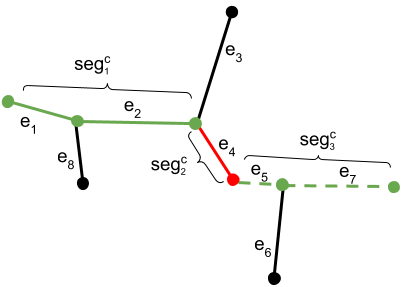
\includegraphics[height=2in]{imagenes/ant_segments_complex_case_block.png}
	    \caption{El camino de la hormiga $c$ no puede pasar de la arista $e_4$ en el caso que la penalizaci\'on no tenga relaci\'on con el segmento que precede a esa arista.}
        \label{fig:segmentComplexCaseBlocked}
    \end{subfigure}
    \caption{Funcionamiento de la propuesta de penalizaci\'on de anti-feromonas con segmentos y recorrido inverso. Por simplicidad se supone que la penalizaci\'on de $\tau_{ij}$ solo una vez es suficiente para eliminar la posibilidad de elegir una arista $c_{ij}$. En este ejemplo, los caminos $a$ y $b$ se desechan por evaluarse como de mala calidad. El camino es penalizando en $e_4$ respecto al segmento que lo precede. El camino $c$ puede seleccionar la arista $e_4$ ya que esta arista no se encuentra penalizada con respecto al segmento $seg^{c}_1$, pudiendo luego agregar el segmento $seg^{c}_3$.Fuente: Elaboraci\'on Propia.}
    \label{fig:segmentComplexCase}
\end{figure*}

Un caso particular en el que esta propuesta puede sufrir del mismo problema de bloqueo de soluciones, es al momento que un segmento formado por s\'olo una arista se encuentre entre 2 segmentos. Este situaci\'on, reflejada en la Figura \ref{fig:segmentComplexCaseB}, implica que la penalizaci\'on que involucre un segmento de una sola arista, como el segmento $seg^{a}_2$, puede generar un bloqueo para los recorridos de otras hormigas. Este tipo de segmentos puede generarse a partir de aristas que forman un \'angulo que pertenece al rango $]\theta, Max\_Angle]$ con cada uno de sus vecinos, como es el caso de la arista $e_4$ en el ejemplo.

Para subsanar aquel caso, a los segmentos de s\'olo una arista se le a\~naden las aristas del segmento que lo precede con el objetivo de evitar que el an\'alisis sea s\'olo entre 2 aristas. As\'i, el segmento $seg^{a}_2$ pasa a ser formado por las aristas $e_3$ y $e_4$, evitando el bloqueo de la hormiga $b$.

\clearpage

%Este situaci\'on, reflejada en la Figura \ref{fig:segmentComplexCaseH}, implica que la penalizaci\'on efectuada a los caminos de las hormigas $a$ y $b$ pueden generar un bloqueo del camino de la hormiga $c$, dado que tras la penalizaci\'on efectuada en la evaluaci\'on de $b$, se tiene un segmento conformado solo por la arista $e_4$, la que forma un \'angulo que pertenece al rango $]\theta, Max\_Angle]$ con cada uno de sus vecinos.

%Si el camino continua siendo de .... otras hormigas pueden intentar iterativamente 
%explicar q la penalizacion es solo necesaria en soluciones de calidad intermedia


 \begin{figure*}[t]
    \centering
    \begin{subfigure}[t]{0.48\textwidth}
        \centering
        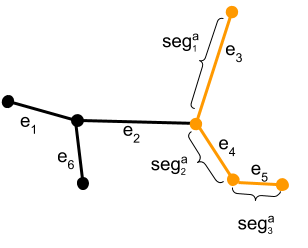
\includegraphics[height=2in]{imagenes/ant_segments_complex_case_B1.png}
        \caption{Camino de una hormiga $a$ que contiene las aristas $e_3$, $e_4$ y $e_5$.}
        \label{fig:segmentComplexCaseB1}
    \end{subfigure}%
    ~ \hspace{0.5cm}
    \begin{subfigure}[t]{0.48\textwidth}
        \centering
        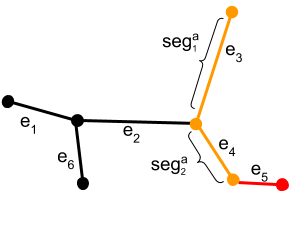
\includegraphics[height=2in]{imagenes/ant_segments_complex_case_B2.png}
        \caption{Penalizaci\'on del camino de la hormiga $a$ en la arista $e_5$ con respecto al segmento $seg^{a}_2$ conformado solo por la arista $e_4$.}
        \label{fig:segmentComplexCaseB2}
    \end{subfigure}

\vskip\baselineskip
    \begin{subfigure}[t]{0.48\textwidth}
        \centering
        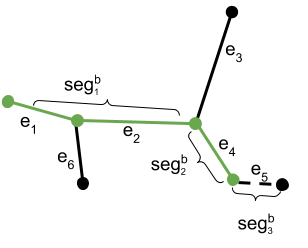
\includegraphics[height=2in]{imagenes/ant_segments_complex_case_B_blocked.png}
	    \caption{Camino de una hormiga $b$ que contiene las aristas $e_1$, $e_2,$ y $e_4$. El camino $b$ no puede agregar la arista $e_5$ debido a que se encuentra penalizada para el segmento conformado por la arista $e_4$, que corresponde al $seg^{a}_2$.}
        \label{fig:segmentComplexCaseBBlocked}
    \end{subfigure}%
    ~ \hspace{0.5cm}
    \begin{subfigure}[t]{0.48\textwidth}
        \centering
        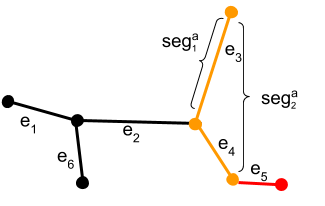
\includegraphics[height=2in]{imagenes/ant_segments_complex_case_B2_extended.png}
        \caption{Soluci\'on propuesta para los segmentos de solo 1 arista no causen bloqueos como el que afecta a la hormiga $b$, mediante la extensi\'on del segmento, a\~nadiendo el segmento anterior.}
        \label{fig:segmentComplexCaseB2Extended}
    \end{subfigure}

    \caption{Caminos de las hormigas $a$ y $b$. Para evitar que la penalizaci\'on sobre $e_5$ por el segmento que lo precede, $seg^{a}_2$, bloquee el camino $b$, se modifica el inicio del segmento asociado a la penalizaci\'on, incorporando las aristas del segmento previo, $seg^{a}_2$. As\'i se mantiene la l\'ogica de asociar la penalizaci\'on no solo a la arista sino que tambi\'en al segmento que la precede. Estos casos suceden para aristas como $e_4$, que forman \'angulos en el rango $]\theta, Max\_Angle]$ con todas sus aristas vecinas, quedando solas en un segmento de largo 1. Fuente: Elaboraci\'on Propia.}
    \label{fig:segmentComplexCaseB}
\end{figure*}


%La perdida de exploraci\'on tambi\'en sucede en el caso que el segmento $seg_{n+1}$ contenga solo 1 arista y no sea el segmento en el que finaliza el recorrido de la hormiga. En aquel caso, la \'unica arista de $seg_{n+1}$ se transforma en un cuello de botella para la exploraci\'on debido a que penaliza de forma indiscriminada a todas las hormigas que pasen por ah\'i, independientemente del \'angulo que forme con otras aristas o componentes. 

%Luego, mediante la anti-feromona se relaciona un segmento $seg^{a}_n \subset s$ y la componente de soluci\'on $c_{ij} \in seg_{n+1} \in s$, donde la elecci\'on de la arista o componente $c_{ij}$ despu\'es de haber elegido las aristas pertenecientes a $seg_n$ origina una soluci\'on de mala calidad. 

\clearpage

\section{Criterios para la actualizaci\'on de anti-feromonas}

La anti-feromona se aplica sobre hormigas que han finalizado su recorrido, cuya calidad normalizada se encuentre entre $[Max\_Score/2, Max\_Score[$, las que tienden a ser caminos de calidad intermedia. Aquello implica que al menos un par de las aristas del recorrido forman un \'angulo que pertenece al rango intermedio $]\theta, Max\_Angle]$, necesitando un an\'alisis adicional para determinar si corresponde a una soluci\'on de buena calidad. Este an\'alisis consta de dos criterios que se aplican sobre todas las c\'elulas cuyos filamentos se deseen individualizar, mientras que existe un tercer criterio adicional aplicable s\'olo en el caso de las neuronas. Los dos criterios generales, o criterios comunes, consisten en evaluar la curvatura del recorrido, como tambi\'en la magnitud del desplazamiento entre la proyecci\'on de un segmento con respecto a un segmento adyacente. El criterio adicional relativo solo a las neuronas busca validar que la finalizaci\'on del recorrido no sea en una arista con uno de sus nodos con grado 1. Es decir, esta arista final no debe cumplir con el primer criterio de la heur\'istica de asignaci\'on de aristas iniciales, descrita en la secci\'on \ref{subsubsec:antTourInit}.
%El an\'alisis adicional se separa en evaluaciones comunes que no dependen de la c\'elula observada, agregando posteriormente las evaluaciones particulares.

\subsection{Curvatura de una soluci\'on}


La curvatura del recorrido de una hormiga $a$ se obtiene al calcular el \'angulo entre la proyecci\'on de un vector con respecto a otro. Los vectores son formados por el nodo inicial del camino, $v^{a}_1$, el centro de masa del recorrido de la misma hormiga, $mc^{a}$, y el nodo final, $v^{a}_n$. As\'i, se definen $\Vec{p} = v^{a}_1 - mc^{a}$ y $\Vec{q} = mc^{a} - v^{a}_n$.



%Estos vectores, definidos como $\Vec{p} = $ y $\Vec{q}$, se generan a partir d Corresponden a $\Vec{p}$ los elementos $v^{a}_1$ y $mc^{a}$, mientras que $\Vec{q}$ es formado por $mc^{a}$ y $v^{a}_n$.


El \'angulo entre la proyecci\'on de $\Vec{p}$ y $\Vec{q}$ no debe superar el valor que resulta al multiplicar el \'angulo $\theta$ por el factor {\it Max\_Axial\_Displacement}. Este factor permite flexibilizar la tolerancia de la curvatura en base a $\theta$. Si el recorrido de la hormiga tiene un \'angulo igual o mayor al umbral, implica que la soluci\'on encontrada es demasiado curva para representar un filamento, por lo que es penalizada y descartada. Un ejemplo se puede observar en la Figura \ref{fig:antCurvCase}, con el camino formado por las aristas $e_3$, $e_4$, $e_5$ y $e_7$, que presenta una curvatura muy marcada, por lo que es penalizado y descartado. La actualizaci\'on del valor de $\tau_{ij}$ mediante el criterio de curvatura se refleja en la ecuaci\'on \ref{eq:antiPheroSAP_Angle}.
%\begin{equation}
%    \label{eq:antiPheroSAP_Angle}
%    \tau_{ij} \leftarrow \tau_{ij} \cdot \gamma \quad \forall \langle c_{ij},seg_{n}\rangle > \textrm{Max\_Axial\_Displacement}
%\end{equation}

\begin{equation}
    \tau_{ij} \leftarrow
        \begin{cases}
        \tau_{ij} \cdot \gamma \text{ si } \measuredangle(proy(\Vec{p}), \Vec{q}) \geq \theta \cdot \text{Max\_Axial\_Displacement},\\[3ex]
        
        \text{0 si } \tau_{ij} \leq 0.25, \\[3ex]
        \tau_{ij} \quad \text{en otro caso.}
        \end{cases}
    \label{eq:antiPheroSAP_Angle}
\end{equation}

\begin{figure}[h]
    \centering
    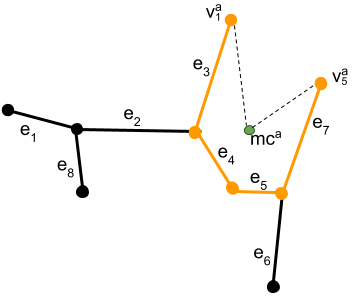
\includegraphics[scale=0.8]{imagenes/ant_curvature_case.png}
    \caption{Curvatura de un camino de una hormiga $a$ que contiene las aristas $e_1$, $e_3$, $e_4$ y $e_7$. $\Vec{p}$ es la proyecci\'on del vector formado por $v^{a}_1$ y $mc^{a}$. $\Vec{q}$ es el vector formado por $mc^{a}$ y $v^{a}_5$. Para cumplir con el rriterio de curvatura, el \'angulo entre la proyecci\'on de $\Vec{p}$ y $\Vec{q}$ debe ser menor a $\theta \times Max\_Axial\_Displacement$ para no descartar la soluci\'on. }
    \label{fig:antCurvCase}
\end{figure}

\begin{figure*}[h]
    \centering
    \begin{subfigure}[t]{0.45\textwidth}
        \centering
        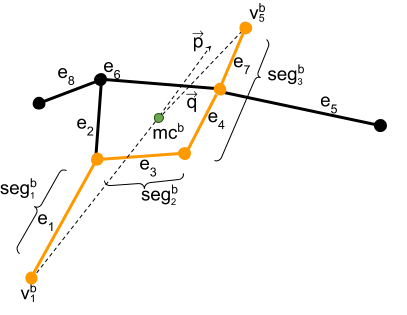
\includegraphics[height=2.5in]{imagenes/ant_segmentMagnitude_case.png}
        \caption{Soluci\'on $b$ cumple con el criterio de curvatura, pero la proporci\'on de la magnitud entre los segmentos $seg^{b}_2$ y $seg^{b}_1$ con respecto a su \'angulo puede indicar que no es una buena soluci\'on.}
        \label{fig:antCurvNotEnough}
    \end{subfigure}
    ~ \hspace{0.5cm}
    \begin{subfigure}[t]{0.45\textwidth}
        \centering
        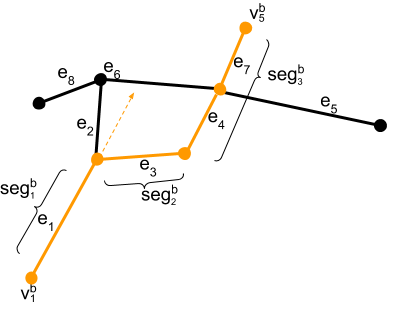
\includegraphics[height=2.5in]{imagenes/ant_segmentMagnitude_case_2.png}
        \caption{An\'alisis del desplazamiento del segmento $seg^{b}_2$ con respecto a la proyecci\'on del $seg^{b}_1$ denota un giro brusco y pronunciado que podr\'ia no respetar la rigidez de algunos tipos de filamentos.}
        \label{fig:antMaxDisplExample}
    \end{subfigure}%
    \caption{Criterio de magnitud y pronunciaci\'on del desplazamiento entre 2 segmentos contiguos. (a) El criterio de curvatura puede no ser suficiente por si mismo para descartar todas las soluciones de mala calidad. (b) La informaci\'on a priori respecto a la rigidez de un filamento permite descartar soluciones que presenten cambios demasiado pronunciados entre los segmentos que la conforman. Fuente: Elaboraci\'on Propia.}
    \label{fig:antMaxDisp}
\end{figure*}

\subsection{Magnitud de desplazamiento entre segmentos}
%agregar referencia? tindemans rod straightness \cite{hawkins2010model} of MTs o 
El an\'alisis respecto a la magnitud del desplazamiento entre la proyecci\'on de un segmento en relaci\'on a sus segmentos vecinos se fundamenta en la rigidez que algunos tipos de filamentos como los microt\'ubulos y los filamentos de actina poseen \cite{stam2017filament}\cite{civalek2011bending}. El criterio de m\'aximo desplazamiento entre segmentos contiguos consiste en limitar la magnitud del movimiento que representa un segmento en relaci\'on al \'angulo que forma con sus segmentos adyacentes. Esto permite descartar soluciones que respeten el criterio de curvatura, pero que presentan movimientos pronunciados que sobrepasan la rigidez esperada de un filamento.

%El criterio de rigidez consiste en analizar los segmentos con respecto a la totalidad de sus predecesores, comenzando por el \'ultimo segmento recorrido por la hormiga, es decir, desde el extremo final de la soluci\'on. 
A partir de cada par de segmentos vecinos en una soluci\'on, se  selecciona el segmento de mayor longitud, el que servir\'a para determinar cual es el movimiento proyectado con respecto al movimiento reflejado por el segmento de menor longitud. Se define el segmento m\'as largo entre ambos segmentos comparados en un camino $a$ como $seg^{a}_{iMax}$ , mientras que el segmento menor es $seg^{a}_{jMin}$. El \'angulo entre $seg^{a}_{jMin}$ y la proyecci\'on de $seg^{a}_{iMax}$ se define como 
$\measuredangle seg^{a}_{pMaxMin}$ por simplicidad. En el caso de que el \'angulo $\measuredangle seg^{a}_{pMaxMin}$ este en el rango $[0, \theta]$ se entiende que se respeta el criterio de m\'aximo desplazamiento.


Si el \'angulo es mayor a $\theta$, se espera que la magnitud del segmento menor $seg^{a}_{jMin}$ multiplicada por el seno de $\measuredangle seg^{a}_{pMaxMin}$ sea menor al umbral que delimita al desplazamiento m\'aximo entre segmentos, definido como el m\'ultiplo de $seg^{a}_{iMax}$ por el 10\% de {\it Max\_Axial\_Displacement}. Lo anterior se ilustra en la Figura \ref{fig:antMaxDisp}, y se describe la actualizaci\'on de $\tau_{ij}$ en la ecuaci\'on \ref{eq:antiPheroSAP_Axial}.

% como $s_{max} = \max(\norm{seg_{n}}, \norm{seg_{1,n-1}})$, para calcular el \'angulo suplementario que forma con respecto al otro miembro del par, definido como $s_{min}$. El \'angulo suplementario, $\measuredangle supl(s_{max},s_{min})$ es el equivalente a calcular el \'angulo entre la proyecci\'on de $s_{max}$ y $s_{min}$.

\begin{equation}
    \tau_{ij} \leftarrow
        \begin{cases}
        \begin{split}
         \tau_{ij} \cdot \gamma \text{ si } & \sin(\measuredangle seg^{a}_{pMaxMin}) > seg^{a}_{iMax} \cdot 0.1 \cdot \text{Max\_Axial\_Displacement} \\ & \land \measuredangle seg^{a}_{pMaxMin}) > \theta,
        \end{split}
        \\[3ex]
        
        \text{0 si } \tau_{ij} \leq 0.25, \\[3ex]
        \tau_{ij} \quad \text{en otro caso}.
        \end{cases}
    \label{eq:antiPheroSAP_Axial}
\end{equation}

%Luego $s_{min}$ es multiplicado por el seno del \'angulo suplementario, estableciendo el desplazamiento con respecto al eje que forma $s_{max}$ y su proyecci\'on. El umbral que delimita al desplazamiento calculado previamente se define como el m\'ultiplo de $s_{max}$ por 10\% de {\it Max\_Axial\_Displacement}. 

%Si el \'angulo suplementario es menor a $\theta$, se puede declarar que se cumple el criterio de rigidez. Lo anterior se refleja en la ecuaci\'on \ref{eq:antiPheroSAP_Axial}. 


%Esta propiedad puede ser utilizada para delimitar como un segmentos de una hormiga se relaciona con el resto de la soluci\'on, ya que estos ser\'ia un reflejo indirecto de los movimientos din\'amicos de un filamento en el tiempo, capturados en un punto a trav\'es de una imagen. 
%La rigidez de un filamento puede describirse mediante la relaci\'on que existe entre un segmento de una hormiga, con respecto a todos los segmentos que lo preceden. 


\subsection{Criterio espec\'ifico para neuronas}
\label{subsec:pheroNeurons}

%Si un camino cumple con ambas criterios de penalizaci\'on comunes, y se trata de una c\'elula distinta a una neurona, la soluci\'on avanza hac\'ia el an\'alisis del m\'etodo de b\'usqueda no local. En cambio,
Si la c\'elula observada es una neurona, corresponde aplicar el criterio adicional espec\'ifico a esta c\'elula. Este criterio adicional se fundamenta en que el comportamiento esperado de los filamentos en una neurona permite caracterizar los lugares desde los cuales nuevos filamentos pueden generarse. As\'i, es necesario validar que los filamentos de una neurona parten del {\tt soma} o centro de la misma, y que filamentos posteriores que no comiencen del soma s\'olo pueden nacer a partir de otros filamentos. Un camino que termine en un nodo final de grado de 1 no respeta aquel comportamiento, debido a que en un grafo que representa una red de filamentos de una neurona, los nodos ubicados en el soma o en la intersecci\'on entre filamentos presentan un grado mayor a 1. La penalizaci\'on al valor de $\tau_{ij}$ para este caso particular se refleja en la ecuaci\'on \ref{eq:antiPheroSAP_neuron}.

\begin{equation}
    \tau_{ij} \leftarrow
        \begin{cases}
         \tau_{ij} \cdot \gamma \text{ si } deg(v^{a}_{n}) = 1,  \\[3ex]
        
        \text{0 si } \tau_{ij} \leq 0.25, \\[3ex]
        \tau_{ij} \quad \text{en otro caso}.
        \end{cases}
    \label{eq:antiPheroSAP_neuron}
\end{equation}

%Finalmente, la ecuaci\'on \ref{eq:antiPheroSAP} refleja la aplicaci\'on de las {\it anti-feromonas} sobre el par $\langle c_{ij}$,$ seg_{n}\rangle \forall c_{ij} \in ]\theta, Max\_Angle]$  donde $c_{ij} \in seg_{n+1}$, y cuya elecci\'on dio lugar a $seg_{n+1}$ que se aleja del desplazamiento axial m\'aximo que un filamento puede soportar.



\section{M\'etodo de b\'usqueda no local}
\label{sec:nonLocalSearch}
Una vez que la hormiga termina un recorrido, es posible agregar un m\'etodo de retroalimentaci\'on sobre la calidad del camino construido, basado en l\'ogicas globales/centralizadas que escapan de la b\'usqueda local que realiza cada hormiga. El o los m\'etodos en esta etapa permite extender la l\'ogica con respecto a una metaheur\'istica ACO, y son opcionales, por lo que no siempre son utilizados. 

Para la individualizaci\'on de filamentos, la evaluaci\'on global corresponde a eliminar soluciones candidatas que no aporten informaci\'on nueva, como puede suceder si una soluci\'on se encuentra contenida dentro de otra. Espec\'ificamente, si una soluci\'on $s^{a}$ se conforma por uno o m\'as segmentos y todos estos existen de forma equivalente en otra soluci\'on $s^{b}$, que a su vez puede tener segmentos que no posean equivalencia en $s^{a}$, se cumple que $s^{b}$ contiene a $s^{a}$. Al ser una soluci\'on contenida en otra, $s^{a}$ es redundante, pudiendo descartarse al disminuir su calidad a 0. En el caso que $s^{a}$ y $s^{b}$ sean id\'enticas, se conserva la soluci\'on que se haya construido primero. 
 
%\begin{itemize}
%    \item $\forall seg^{a}_{i} \in s^{a}, i = 1\dots n$
    
%    \item $s^{a} \subseteq s^{b}$
%\end{itemize}

Mediante la comparaci\'on de segmentos equivalentes, esta revisi\'on centralizada busca evitar recorridos con un bajo n\'umero de aristas, especialmente los caminos de 1 arista. Un potencial problema asociado a este m\'etodo se encuentra en el caso de que la solucion descartada, $s^{a}$ en el ejemplo, sea la que representa de mejor forma a un filamento, y que la soluci\'on restante por ende sea una representaci\'on no exacta.
%RIESGO ASOCIADO a overmatch!!

%Si dos soluciones, $s_i$ y $s_j$ de las hormigas $i$,$j$, conformadas solamente por componentes $c_{ij} \in [0, \theta]$  (todos los componentes son de {\it buena calidad}), y que adem\'as eran la \'unica opci\'on posible en cada avance de la hormiga (probabilidad 1 de ser elegidas)
%tal que $s_i \subseteq s_j$ o viceversa, se tiene que una soluci\'on candidata no aporta nueva informaci\'on.

\section{Extracci\'on de informaci\'on para individualizar filamentos}
Previo al uso de la metaheur\'istica ACO para individualizar filamentos, es necesario recabar la mayor cantidad de informaci\'on posible a partir de la imagen, as\'i como del grafo extra\'ido. Adem\'as se debe considerar la incorporaci\'on de informaci\'on espec\'ifica de los filamentos en la c\'elula observada, como el o los comportamientos esperados de estos, las que pueden conocerse previamente a la ejecuci\'on del algoritmo propuesto. A medida que se obtiene m\'as informaci\'on, es posible incorporar en el algoritmo diversas heur\'isticas que permitan acotar el espacio de b\'usqueda.

Como se observa en el cap\'itulo \ref{chap:stateoftheart}, diversas investigaciones obtienen informaci\'on geom\'etrica o topol\'ogica, por lo general a partir de una imagen de filamentos. Para extender la obtenci\'on de informaci\'on topol\'ogica con respecto a otros m\'etodos, es posible utilizar los algoritmos para grafos existentes en la librer\'ia {\it sknw}, que son las implementaciones de algoritmos conocidos para grafos. As\'i, es posible utilizar un algoritmo de centralidad como {\it closeness centrality}, el que calcula la distancia de cada nodo con respecto a lo dem\'as, permitiendo identificar los que se encuentran a la menor distancia de todos.


La relevancia de esta informaci\'on adicional es directa en el caso de las neuronas, siendo utilizada en la seccion \ref{subsec:pheroNeurons}, mientras que puede requerir de an\'alisis adicional por parte de expertos para otros filamentos. La aplicaci\'on del algoritmo {\it closeness centrality} refleja la posibilidad de expandir y/o incrementar el uso de informaci\'on topol\'ogica en el algoritmo propuesto. Un ejemplo de {\it closeness centrality} para filamentos en neuronas y microt\'ubulos se observa en la Figura \ref{fig:ExtraInfoCenterNodes}, en la que se eligieron los 3 nodos con menor distancia a los dem\'as. Luego, el color magenta refleja las aristas que poseen al menos uno de estos nodos, mientras que las aristas en amarillo indican las que no poseen ninguno.
%entrega informaci\'on relevante respecto a la conectividad interna en conjuntos de filamentos.

 \begin{figure*}[h!]
    \centering
    \begin{subfigure}[t]{0.48\textwidth}
        \centering
        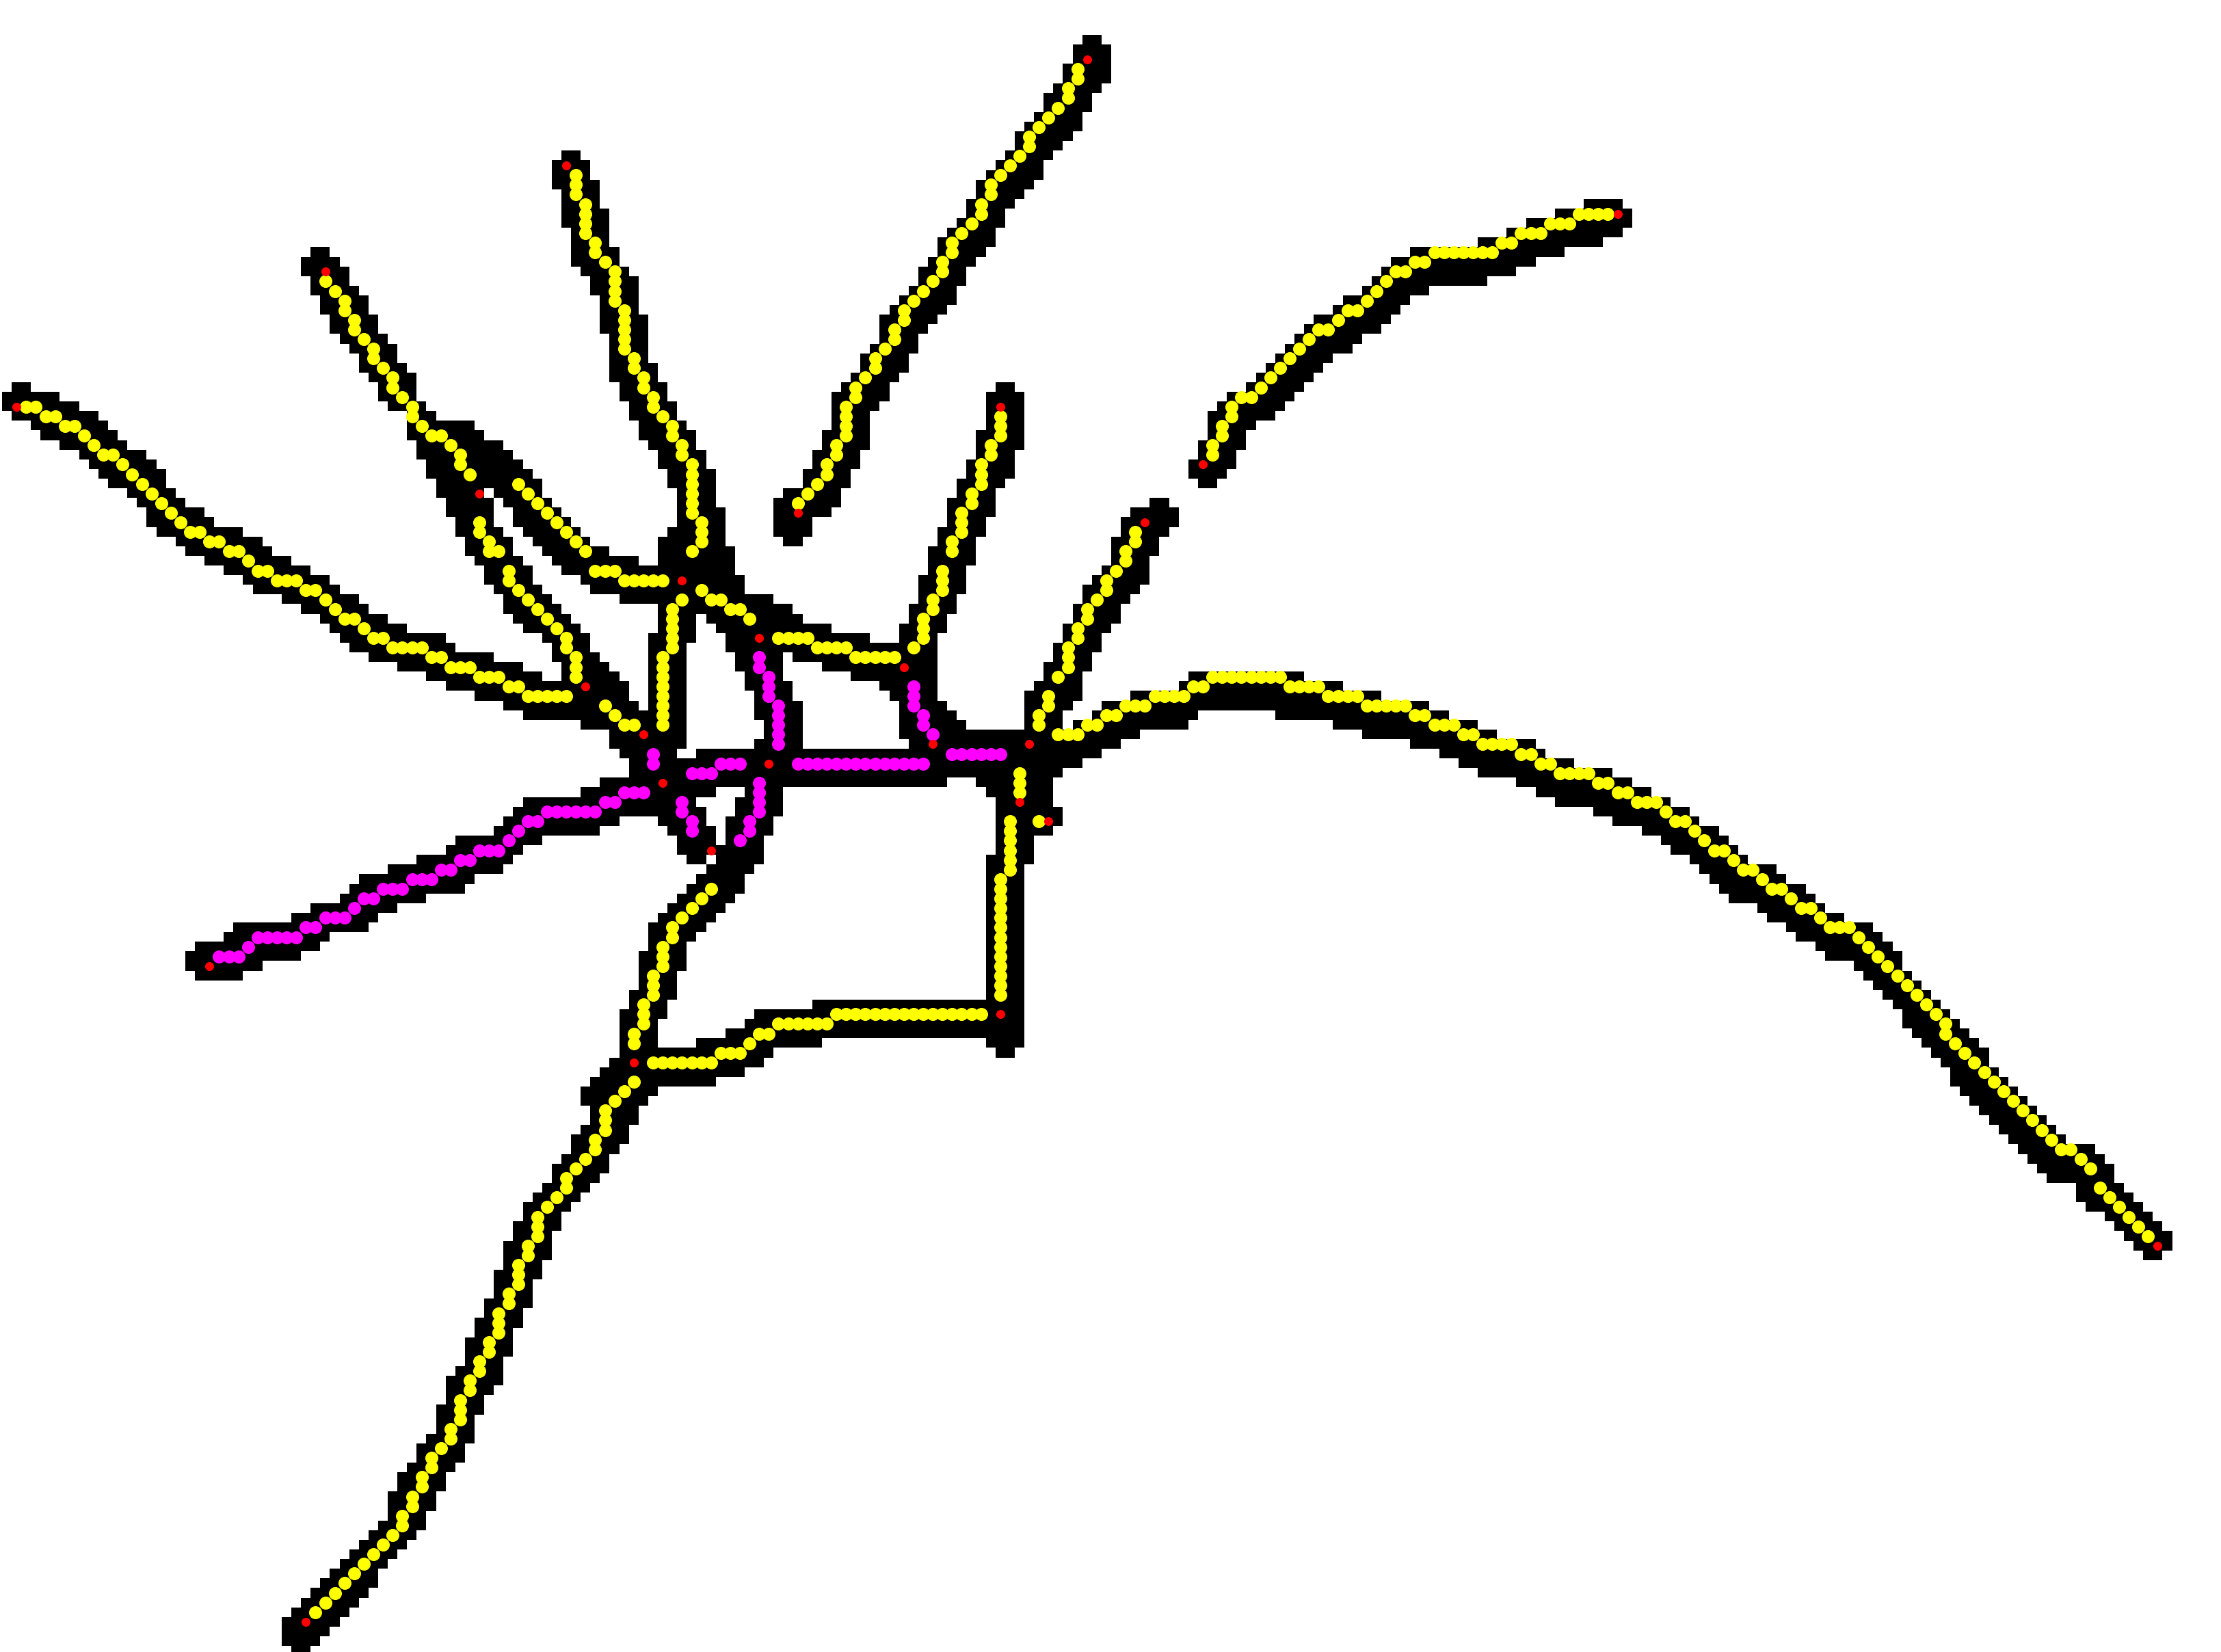
\includegraphics[height=2in]{imagenes/50-ROIs-Spinning-Marchantia-somaEdges.png}
        \caption{Uso del algoritmo {\it closeness centrality} en un grupo de microt\'ublos }
        \label{fig:SpinningCenterNodes}
    \end{subfigure}%
    ~ \hspace{0.5cm}
    \begin{subfigure}[t]{0.48\textwidth}
        \centering
        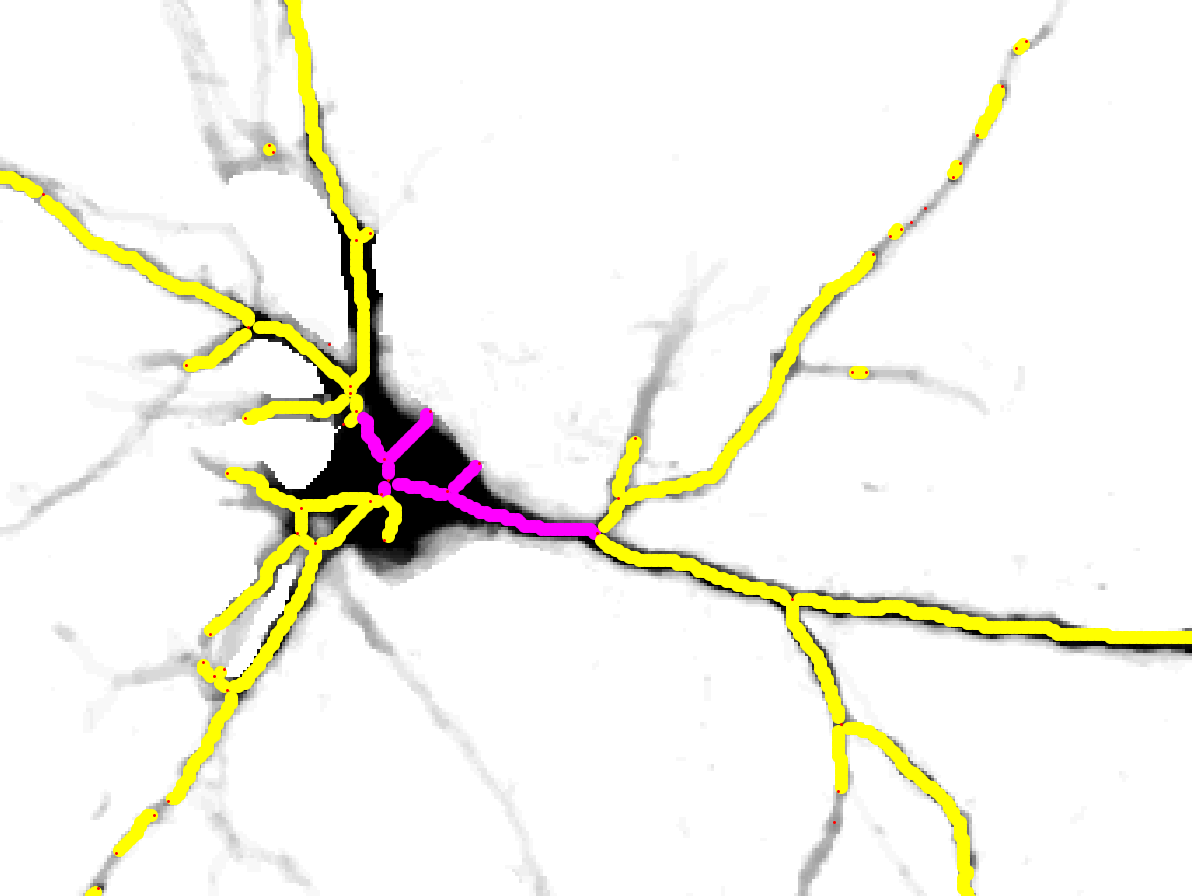
\includegraphics[height=2in]{imagenes/Porta18-3a1-somaEdges.png}
        \caption{Uso del algoritmo {\it closeness centrality} para reflejar nodos y aristas centrales, las que pueden corresponder a la secci\'on del soma en una neurona.}
        \label{fig:Porta18SomaNodes}
    \end{subfigure}

    \caption{Ejemplo del algoritmo {\it closeness centrality} eligiendo los 3 nodos con menor distancia a los dem\'as nodos. El color magenta indica que aristas poseen al menos uno de estos 3 nodos. En el caso de una neurona, permite asociar una o m\'as aristas a una secci\'on espec\'ifica como el soma. Fuente: Elaboraci\'on Propia.}
    \label{fig:ExtraInfoCenterNodes}
\end{figure*}

%info espacial: Ejemplo within, analisis de cruces. Intersect, disjoin y otros, en postgis
Adem\'as de la extracci\'on de informaci\'on previo al uso de la metaheur\'istica ACO, es posible realizar de manera similar, la obtenci\'on de informaci\'on durante la individualzaci\'on de filamentos. Un ejemplo de esto es la informaci\'on espacial con respecto a los nodos y aristas que pueden ser elegidas como parte de un camino. La informaci\'on espacial facilita la comparaci\'on y el an\'alisis entre caminos para identificar casos de cruce, intersecci\'on o solapamiento. En particular, en la secci\'on \ref{sec:nonLocalSearch} se utiliza la consulta espacial {\it within} disponible en la extensi\'on espacial {\it Postgis} para la base de datos {\it PostgreSQL}, para comparar la informaci\'on distinta que entrega un camino con respecto a los dem\'as, considerando que puede existir repetici\'on de caminos entre distintas hormigas. Este an\'alisis resulta simple a trav\'es de una consulta espacial, especialmente a medida que aumentan los caminos a comparar.

El uso de informaci\'on geom\'etrica, topol\'ogica y espacial, repartidos en los m\'etodos de la metaheur\'istica ACO, se enfocan en ampliar las opciones de an\'alisis que puede realizar un experto, as\'i como aumentar la precisi\'on de la individualizaci\'on de filamentos. Nuevas caracter\'isticas que modifiquen la exploraci\'on del espacio de soluciones pueden ser a\~nadidas en el m\'etodo de construcci\'on de soluciones, ampliando el criterio que solo utiliza el \'angulo para determinar o descartar con certeza que 2 aristas pertenezcan o no al mismo filamento. A su vez, en este mismo m\'etodo es posible incorporar nuevas condiciones que delimiten con mayor detalle el inicio o final de un camino.
Por su parte. agregar restricciones adicionales que penalicen caminos finalizados puede realizarse tanto en el m\'etodo de actualizaci\'on de feromonas, en caso de que se trate de restricciones que no requieran comparaci\'on con otras hormigas, o en el m\'etodo de b\'usqueda no local para comparaciones entre 2 o m\'as hormigas.


\vspace{1cm}
En resumen, las condiciones del problema de identificaci\'on de filamentos dan pie a establecer su representaci\'on mediante un problema de optimizaci\'on de restricciones (COP), estando el modelo para la resoluci\'on del COP basado en la metaheur\'istica ACO para su resoluci\'on. La implementaci\'on del modelo de optimizaci\'on presentado es un algoritmo que se encuentra escrito en C++.
\chapter{Metodolog\'ia de evaluaci\'on}
\label{chap:metodologia}
%mostrar métricas, explicar VI brevemente, explicar que no es necesario Structure-Aware rand index ya que los caminos p subconjunto de P', p pertenece P, cumplen por si solos en ser soluciones factibles de segmentos de filamento y que la unión de caminos para formar un filamento, al cumplir con las restricciones también genera solo filamentos factibles
% Dado que Rand y  Jaccard vienen de valores extraidos desde la contingency table, es posible obtener información útil de la mano de precisión, recall y F1

Al basar la individualizaci\'on de filamentos en un m\'etodo que usa un grafo, el resultado obtenido es un conjunto de caminos, donde cada camino es a su vez un conjunto de aristas. El proceso de individualizar filamentos genera una partici\'on o {\it clustering} del grafo, donde las aristas corresponden al {\it data set}, con cada camino representando a un cluster perteneciente al clustering. La partici\'on propuesta por un m\'etodo basado en grafos debe ser comparada con respecto a la partici\'on generada por un experto, a la que nos referiremos como {\it ground truth}. Uno de los requisitos de esta comparaci\'on, es que ambas particiones se refieran al mismo data set, lo que implica que ambas deben realizarse en base al mismo grafo. Adem\'as se debe considerar que el clustering realizado por el experto puede tener una cantidad igual o distinta de clusters con respecto al clustering producido por el m\'etodo a evaluar.



\section{M\'etricas y Medidas}
\label{sec:metricasymedidas}


La comparaci\'on de particiones en donde una corresponde al {\it ground truth} implica que las mediciones a utilizar son del tipo de criterio externo \cite{manning20introduction}. En este tipo de criterio hay \'indices basados en comparaci\'on mediante conteo de pares, como el \'indice {\it Rand} ($\mathcal{R}$), el \'indice {\it Jaccard} ($\mathcal{J}$), y la medida $\mathcal{F}$ tambi\'en conocida como $F1-$Score. Por otra parte, tambi\'en existen m\'etricas del \'area de teor\'ia de la informaci\'on como {\it Variation of Information} o VI para el mismo prop\'osito. Estos m\'etodos ser\'an la base de comparaci\'on de particiones en esta investigaci\'on.

\subsection{\'Indices Rand y Jaccard}

La mayor\'ia de los criterios para comparar particiones mediante conteo de pares suele fundamentarse en el uso de la matriz de confusi\'on, tambi\'en llamada matriz de asociaci\'on o tabla de contingencia \cite{meilua2007comparing}. Esta tabla considera 4 casos en los que puede estar un par de elementos del {\it data set}, que para el caso de la individualizaci\'on de filamentos son pares de aristas, en las particiones $C$ y $C'$:

\begin{itemize}
    \item $N_{11}$: N\'umero de pares que est\'an en el mismo cluster en $C$ y $C'$
    \item $N_{00}$: N\'umero de pares que est\'an en distintos clusters en $C$ y $C'$
    \item $N_{10}$: N\'umero de pares que est\'an en el mismo cluster en $C$ pero no en $C'$
    \item $N_{01}$: N\'umero de pares que est\'an en el mismo cluster en $C'$ pero no en $C$
\end{itemize}

Se tiene que $N_{11} + N_{00} + N_{10} + N_{01} = \frac{n(n-1)}{2}$, con n como el n\'umero de aristas.

Lo definici\'on de los casos utilizados para formar la tabla de contingencia posibilita asociar cada caso con una correspondiente evaluaci\'on de clasificaci\'on como se indica en la tabla \ref{tab:EquivParesClasificacion}.

\begin{table}[h]
    \centering
    \begin{tabular}{|c|c|}
    \hline
        Casos para un par de aristas & Clasificaci\'on \\ \hline
        $N_{11}$ & Verdadero Positivo ({\it True Positive} o TP) \\
        $N_{00}$ & Verdadero Negativo ({\it True Negative} o TN)\\
        $N_{10}$ & Falso Positivo ({\it False Positive} o FP)\\
        $N_{01}$ & Falso Negativo ({\it False Negative} o FN)\\ \hline
    \end{tabular}
    \caption{Equivalencia entre casos para un par de aristas con su respectiva clasificaci\'on}
    \label{tab:EquivParesClasificacion}
\end{table}

La ecuaci\'on \ref{eq:randIndex} expresa que el \'indice Rand puede ser escrito en funci\'on de evaluaciones de clasificaci\'on, lo que lo hace coincidir con la definici\'on de la medida de exactitud ({\it Accuracy}). $\mathcal{R}$ adquiere el valor 0 para particiones totalmente diferentes, subiendo hasta llegar a 1, lo que indica que las particiones son id\'enticas. Algunas cr\'iticas al \'indice Rand se\~nalan la alta sensibilidad que tiene al valor de TN, el que tiende a ser mucho mayor que el resto \cite{ben2001stability}, la existencia de una alta dependencia al n\'umero de clusters \cite{wagner2007comparing}, y que los valores de $\mathcal{R}$ tienden a concentrarse en un intervalo cerca de 1, puntualmente en el rango [0.5, 1] \cite{meilua2007comparing}\cite{vinh2010information}.

\begin{equation}
\mathcal{R}(C,C^{\prime}) = \frac{N_{11} + N_{00}}{n(n-1)/2} = \frac{TP + TN}{TP + TN + FP + FN}
\label{eq:randIndex}
\end{equation}

Por su parte, el \'indice Jaccard es similar al \'indice Rand con la excepci\'on que ignora la clasificaci\'on TN, como se observa en la ecuaci\'on \ref{eq:JaccardIndex}. Su valor tambi\'en oscila entre 0 y 1 para particiones totalmente distintas y particiones id\'enticas respectivamente. Una de las cr\'itica es que puede entregar resultados no confiables para data sets muy peque\~nos.

\begin{equation}
\mathcal{J}(C,C^{\prime}) = \frac{N_{11}}{N_{11} + N_{01} + N_{10}} = \frac{TP}{TP + FP + FN}
\label{eq:JaccardIndex}
\end{equation}

La ventaja que presentan $\mathcal{R}$ y $\mathcal{J}$ sobre VI radica en que estos \'indices si pueden considerar casos de superposici\'on.

\subsection{Variation of Information}
La m\'etrica VI definida en \cite{meilua2007comparing} se fundamenta en la informaci\'on asociada a la entrop\'ia de las particiones a comparar, as\'i como en la informaci\'on mutua que comparten. El rango de valores de VI comienza en 0 para 2 particiones iguales, llegando a $\log n$ para particiones absolutamente distintas, con $n$ como el n\'umero de elementos del data set. En la ecuaci\'on \ref{eq:VI} el t\'ermino $H(C,C^{\prime})$ hace referencia a la informaci\'on que la partici\'on $C$ pierde al pasar a $C^{\prime}$. De forma similar, $H(C^{\prime},C)$ indica la informaci\'on que se gana al pasar de $C$ a $C^{\prime}$.

\begin{equation}
VI(C,C^{\prime}) = H(C,C^{\prime}) + H(C^{\prime},C)
\label{eq:VI}
\end{equation}

Uno de los problemas de VI es que esta definida de forma clara s\'olo para particiones que no se superponen entre s\'i \cite{breuer2015define}.

\subsection{Mediciones adicionales}

Mediante la relaci\'on entre los casos en que un par de aristas puede ser asignada y la clasificaci\'on equivalente es posible evaluar el resultado de una partici\'on con respecto al {\it ground truth} con mediciones del \'area de recuperaci\'on de informaci\'on como {\it Precision}, {\it Recall}, las que a su vez son la base para calcular {\it F-Measure}.
Estos c\'alculos entregan mayor informaci\'on sobre el comportamiento de la partici\'on propuesta por el algoritmo a evaluar. 


Otras medidas que se consideran son el porcentaje de cobertura de aristas, el n\'umero de filamentos correctos respecto al total de filamentos propuestos, los tiempos de c\'omputo y la existencia de soluciones no consideradas por otros algoritmos. El porcentaje de cobertura corresponde a la cantidad de aristas contenidas al menos una vez en alguno de los filamentos propuestos.

\section{Im\'agenes Sint\'eticas}

El uso de im\'agenes sint\'eticas se enfoca en la validaci\'on del m\'etodo de optimizaci\'on presentado en el cap\'itulo \ref{sec:modeloOpti}, cuya implementaci\'on se denomina {\sc Phil}, para casos simples que consideren filamentos que se superponen y/o intersectan. Ejemplos de las im\'agenes sint\'eticas utilizadas se observan en las figuras \ref{fig:synth-QFS-7} y \ref{fig:synth-Define-1b}, cada una acompa\~nada de su grafo representativo de la red de filamentos y de su individualizaci\'on manual. La figura \ref{fig:synth-QFS-7-original} corresponde a una imagen sint\'etica obtenida de \cite{qiu2014quantitative}, mientras que la figura \ref{fig:synth-Define-1b-original} es un subconjunto de la figura 1b  en \cite{breuer2015define}. 
%La figura \ref{fig:synth-arbol9} es una de las im\'agenes creadas en base a un programa escrito en Matlab que simula la generaci\'on de filamentos a partir de un filamento inicial, que luego va generando nuevos filamentos mediante ramificaciones, simulando una estructura tipo \'arbol. La figura \ref{fig:synth-redX} representa a un segundo conjunto de im\'agenes creadas a partir de un programa en Matlab que simula una red de filamentos donde cada nodo es de grado 3 o inferior.
% \ref{fig:synth-arbol9} y \ref{fig:synth-redX}

 \begin{figure*}[h!]
    \centering
    \begin{subfigure}[t]{0.3\textwidth}
        \centering
        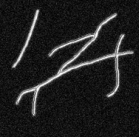
\includegraphics[height=1.5in]{benchImages/Synth-QuantitativeIFS-Fig7_gray.png}
        \caption{Red de filamentos sint\'etica disponible en \cite{qiu2014quantitative}}
        \label{fig:synth-QFS-7-original}
    \end{subfigure}%
    ~ 
    \begin{subfigure}[t]{0.3\textwidth}
        \centering
        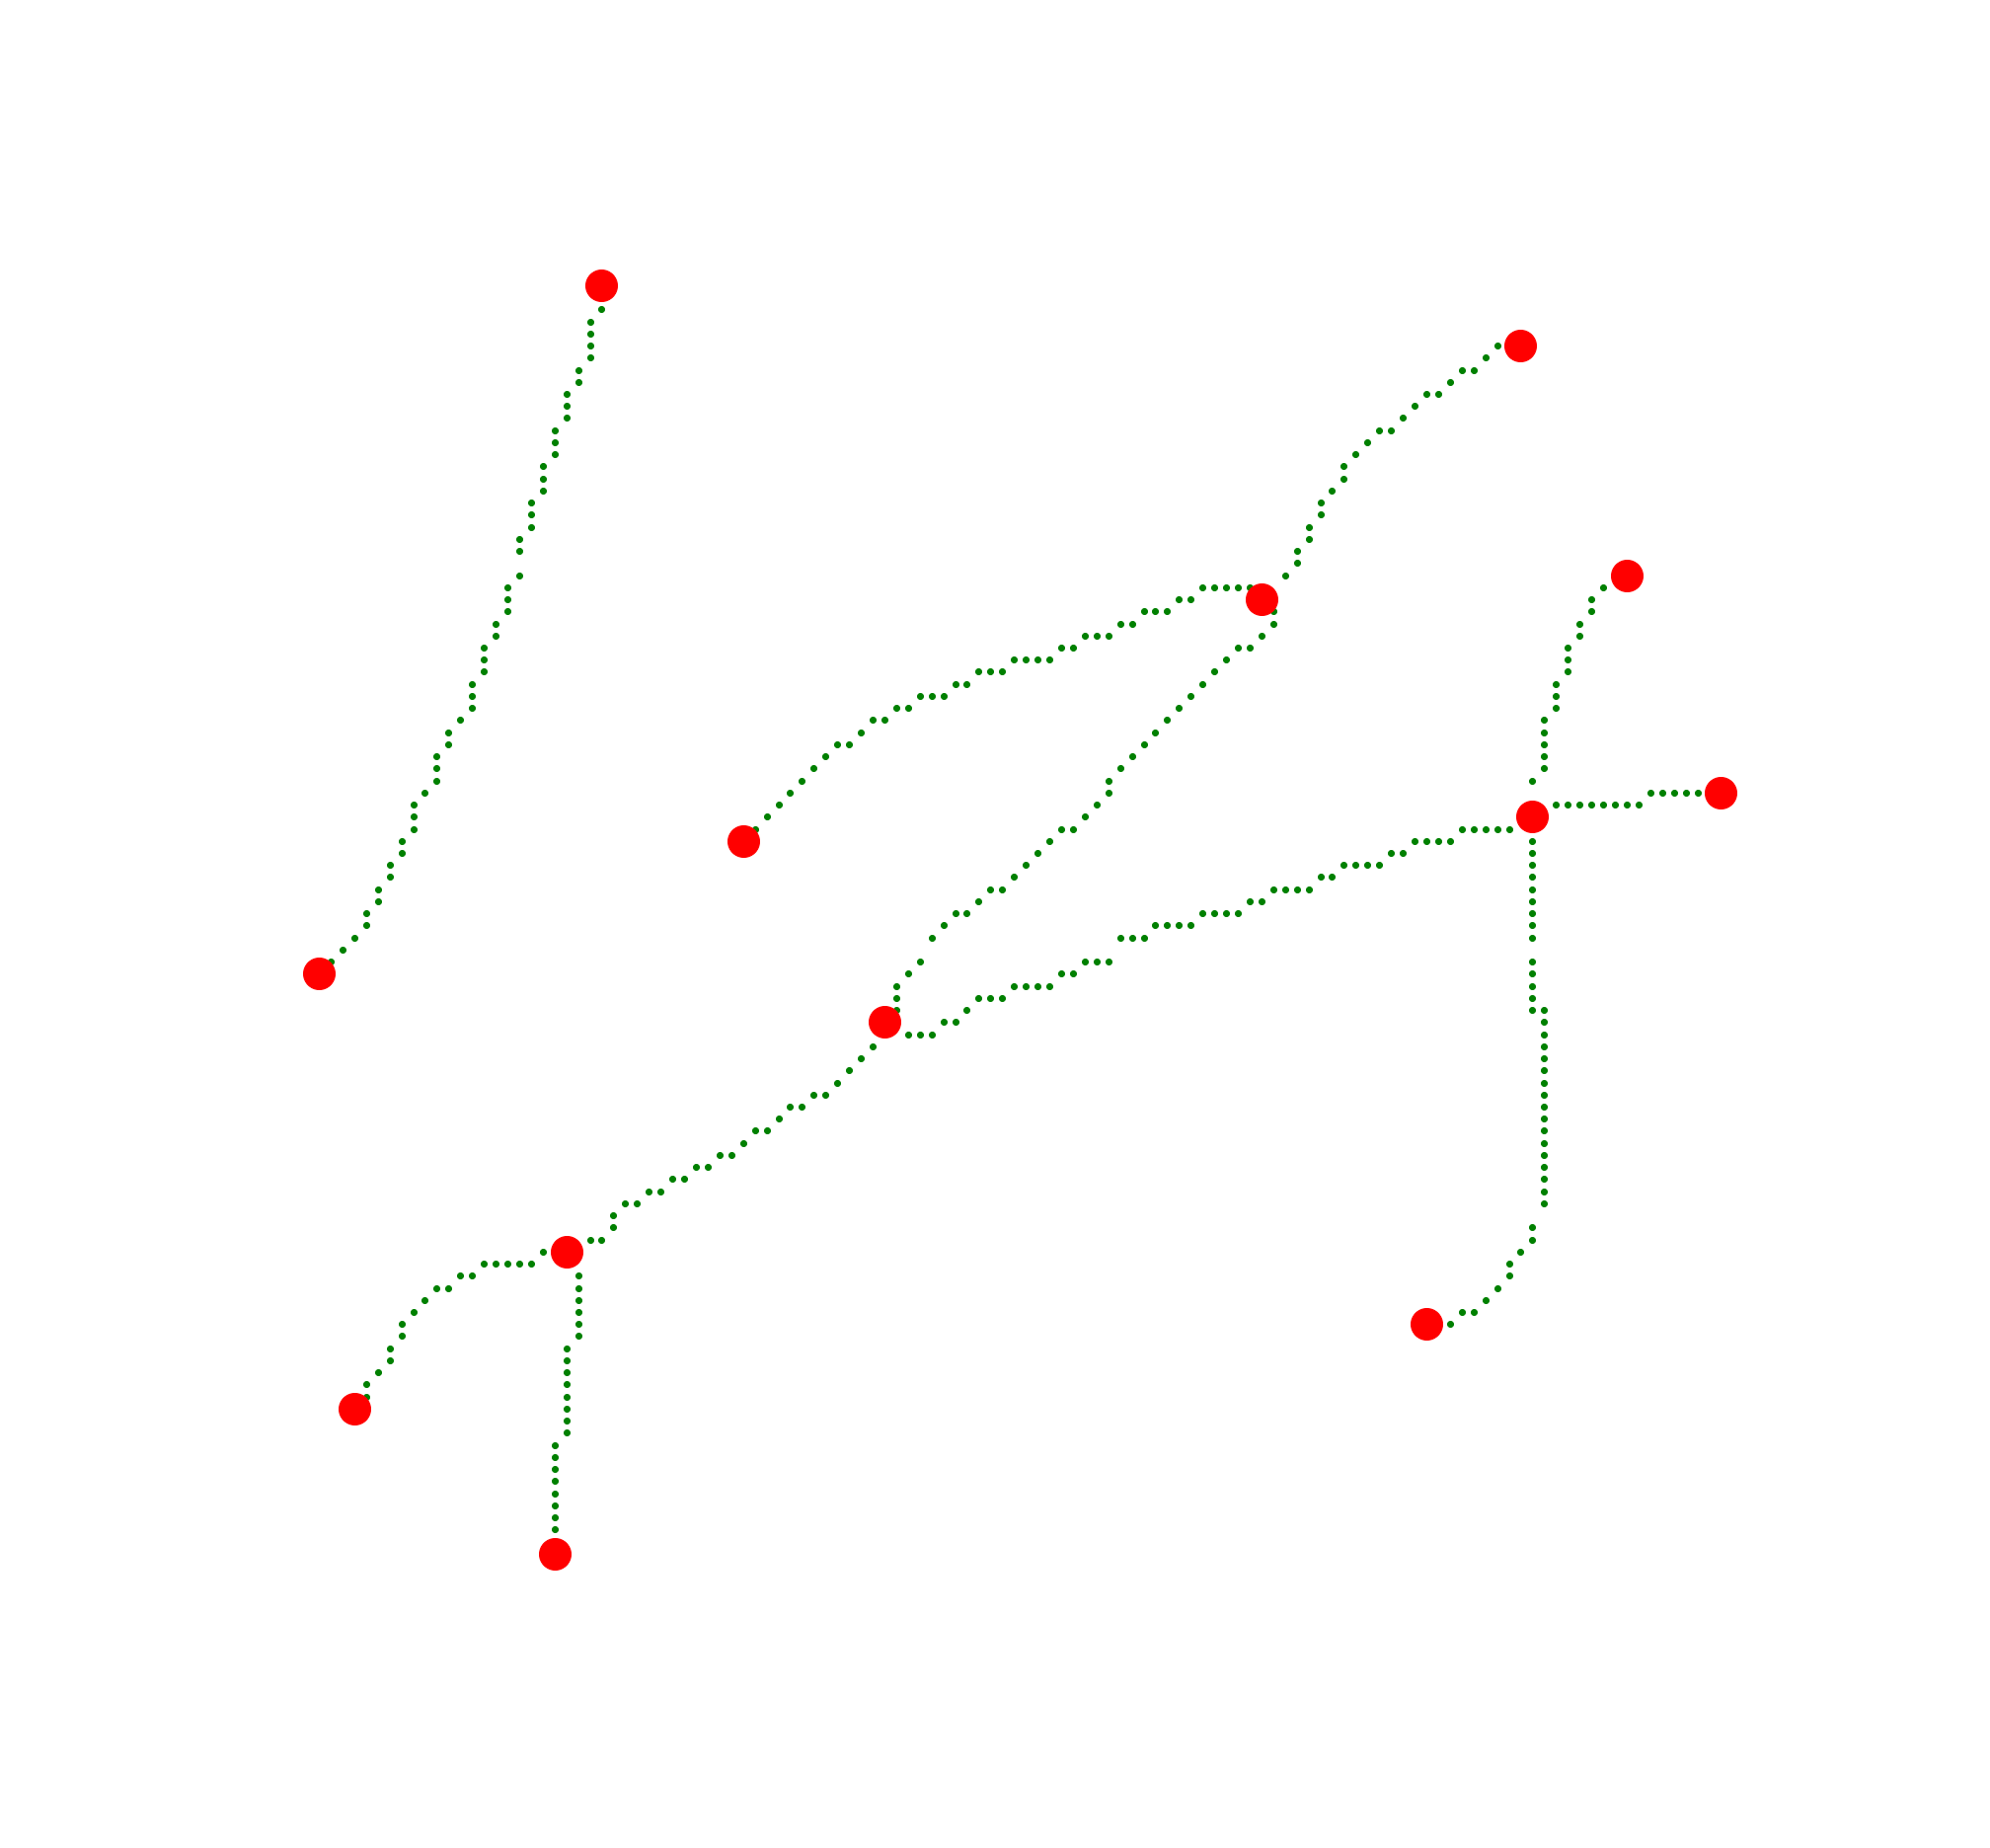
\includegraphics[height=1.5in]{benchImages/Synth-QuantitativeIFS-Fig7_graph_labeled_thick.png}
        \caption{Grafo extra\'ido de la figura \ref{fig:synth-QFS-7-original} utilizando {\it sknw}}
        \label{fig:synth-QFS-7-graph}
    \end{subfigure}
    ~ 
    \begin{subfigure}[t]{0.3\textwidth}
        \centering
        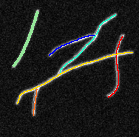
\includegraphics[height=1.5in]{benchImages/Synth-QuantitativeIFS-Fig7_groundTruth.png}
        \caption{Individualizaci\'on manual de la figura \ref{fig:synth-QFS-7-original}}
        \label{fig:synth-QFS-7-graph}
    \end{subfigure}
    \caption{Filamentos sint\'eticos. a) Los colores originales de la figura \ref{fig:synth-QFS-7-original} hacen referencia a la segmentaci\'on de filamentos en vez de la individualizaci\'on, por lo que se utiliza la imagen en escala de grises. b) Grafo de 11 aristas extra\'ido. c) Individualizaci\'n manual utilizando codificaci\'on por colores.}
    \label{fig:synth-QFS-7}
\end{figure*}


 \begin{figure*}[h!]
    \centering
    \begin{subfigure}[t]{0.3\textwidth}
        \centering
        
\includegraphics[height=1.5in]{benchImages/define-weighted-4.png}
        \caption{Red artificial de filamentos extra\'ida de una secci\'on de la figura 1b en \cite{breuer2015define}}
        \label{fig:synth-Define-1b-original}
    \end{subfigure}%
    ~ 
    \begin{subfigure}[t]{0.3\textwidth}
        \centering
        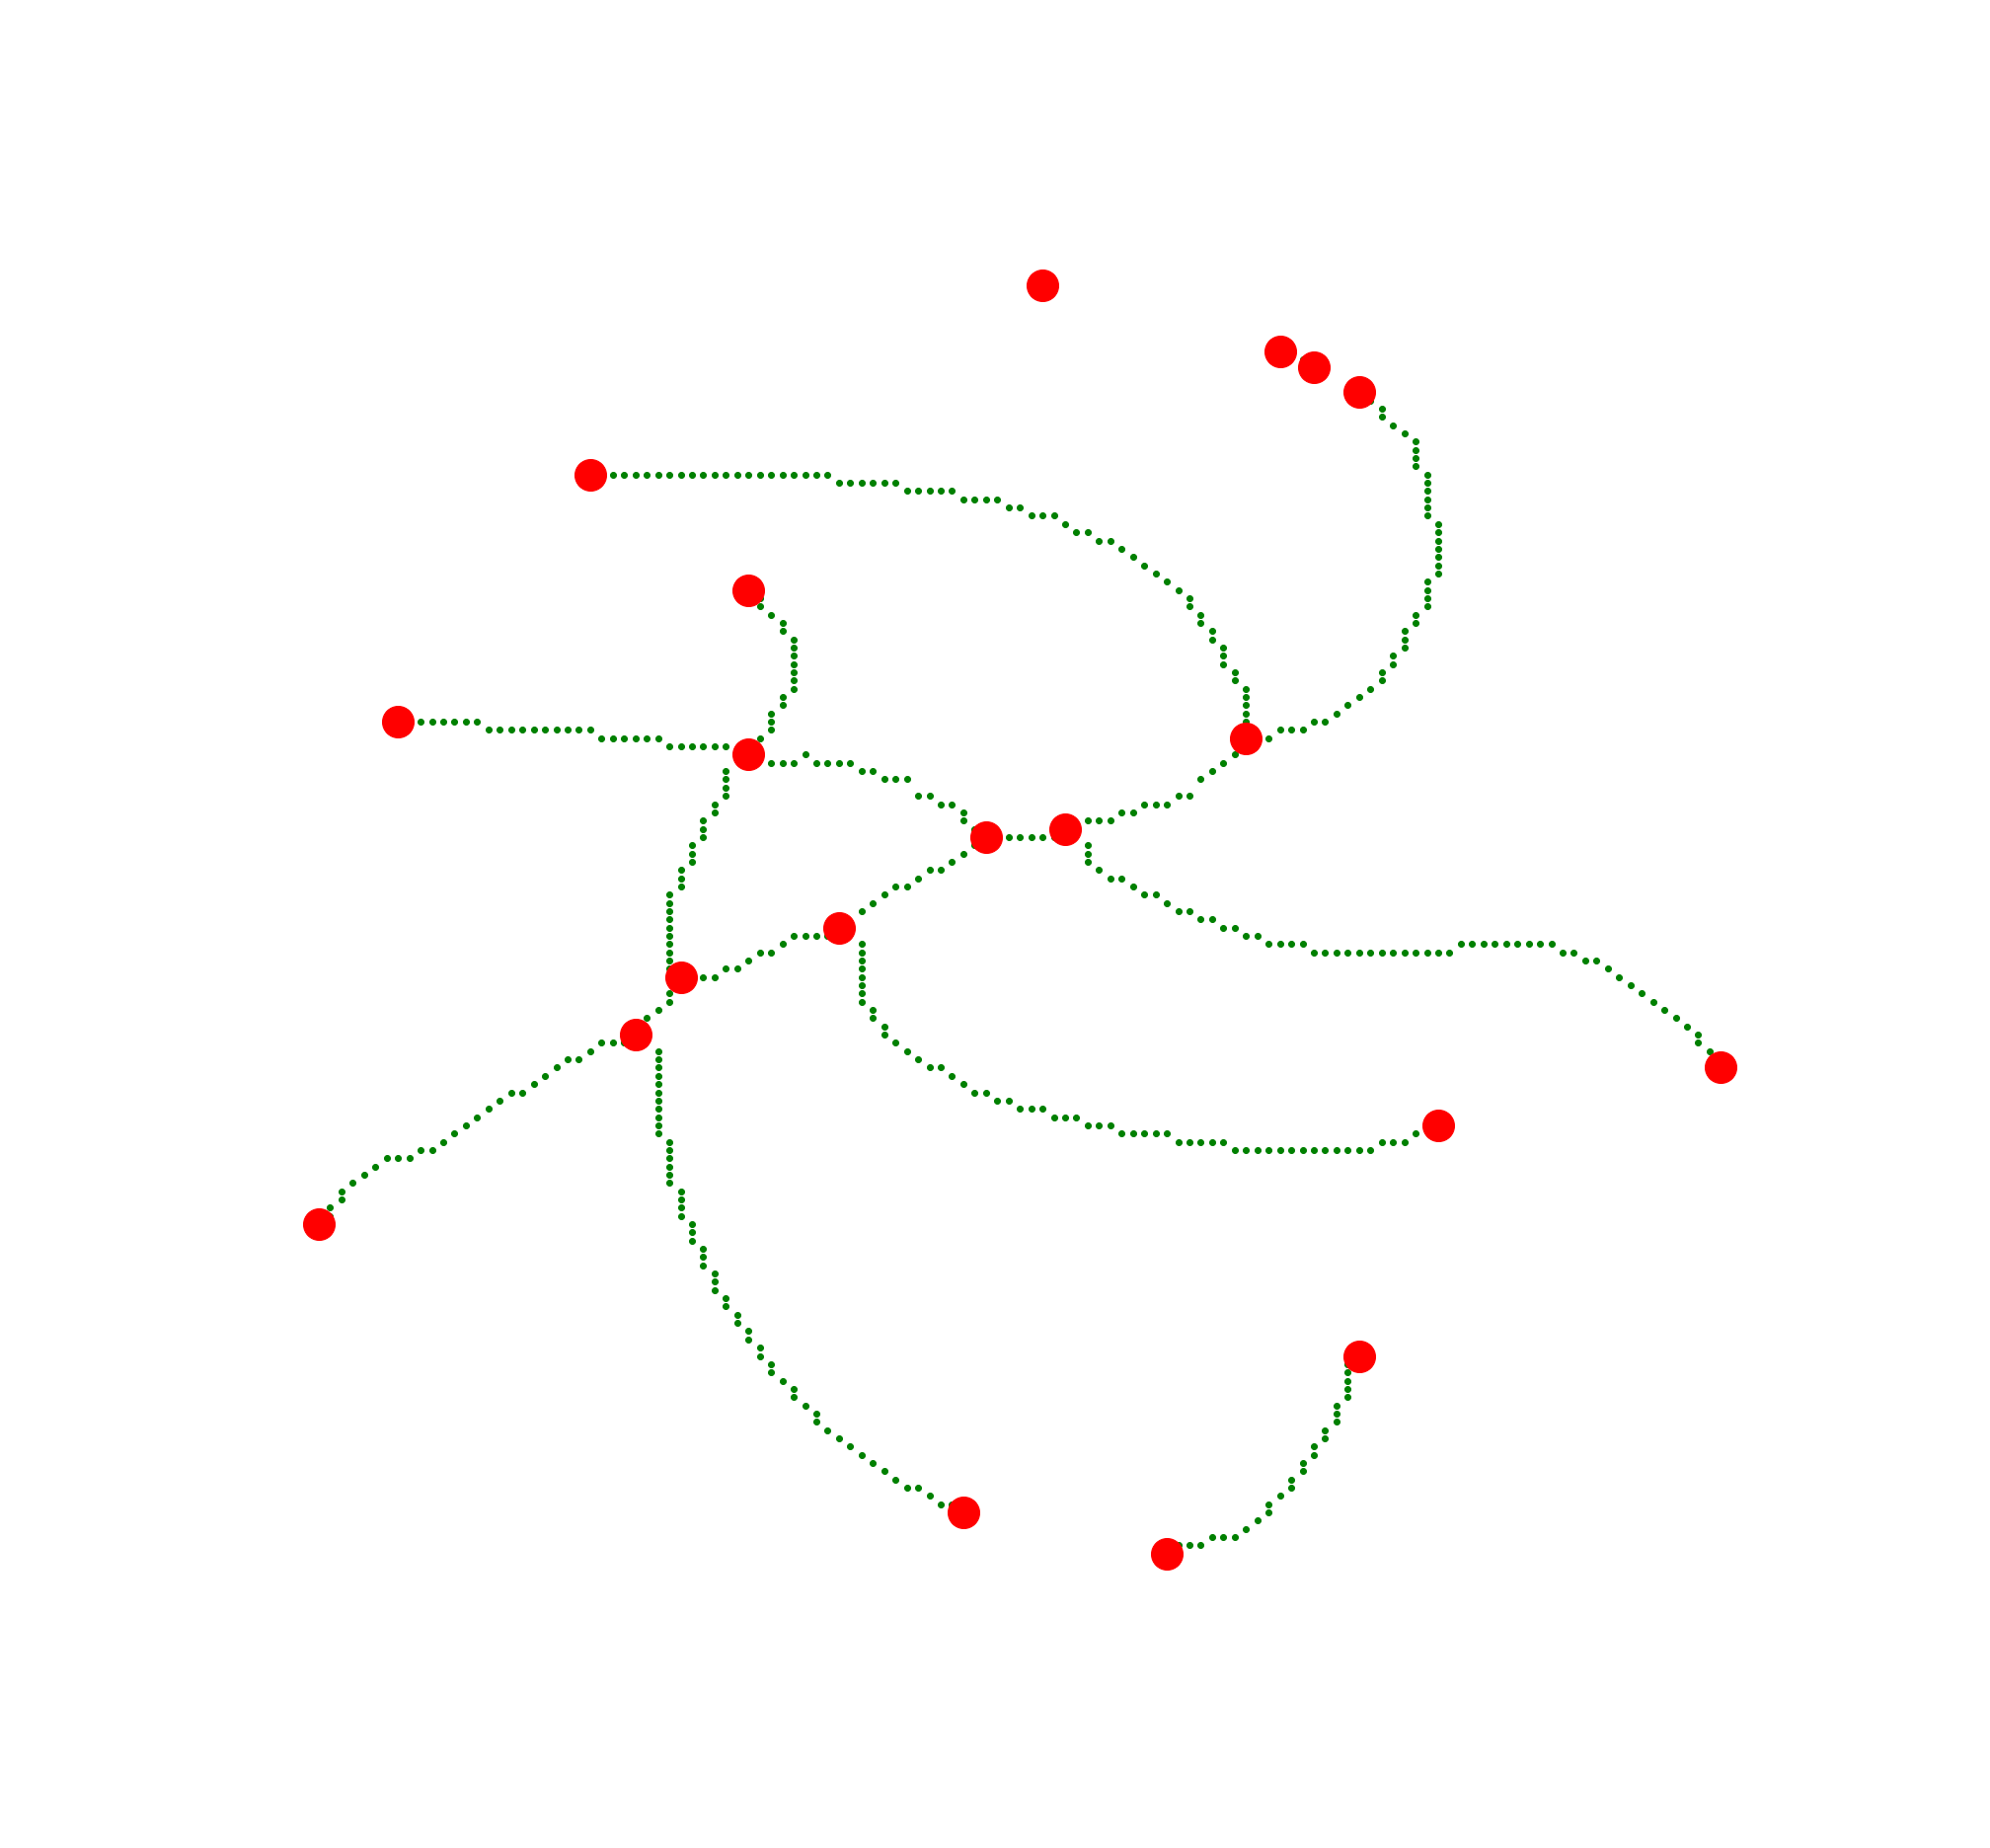
\includegraphics[height=1.5in]{benchImages/define-weighted-4_inv_graph_labeled_thick.png}
        \caption{Grafo extra\'ido de la figura \ref{fig:synth-Define-1b-original} utilizando {\it sknw}}
        \label{fig:synth-Define-1b-graph}
    \end{subfigure}
    ~ 
    \begin{subfigure}[t]{0.3\textwidth}
        \centering
        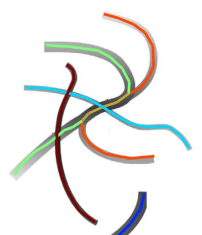
\includegraphics[height=1.5in]{benchImages/define-weighted-4-groundTruth.png}
        \caption{Individualizaci\'on manual de filamentos}
        \label{fig:synth-Define-1b-graph-gt}
    \end{subfigure}
    \caption{Red sin\'etica de filamentos a) Secci\'on de la figura 1b en \cite{breuer2015define}, correspondiente a una red sint\'etica de filamentos que abarca casos de sobreposici\'on y cruce. b) Grafo de 17 aristas. Se puede observar que el final de la arista superior derecha, o una discontinuidad que generando una arista y un nodo adicional. c) Codificaci\'on por colores para individualizar filamentos. La secci\'on de color cafe claro corresponde a un caso de superposici\'on entre dos filamentos.}
    \label{fig:synth-Define-1b}
\end{figure*}

Para la evaluaci\'on, cada imagen sint\'etica se ejecuta en DeFiNe con los par\'ametros base {\tt BFS - Overlapping - Pairwise - Total}, ya que fueron los de mejor resultado en \cite{breuer2015define}, configurando el \'angulo de umbral en 30\textdegree y 60\textdegree. Por su parte, el algoritmo propuesto se ejecuta 5 veces con distintas semillas.

\section{Im\'agenes Reales}
%1.- pasos para la obtenci\'on de los filamentos desde las imagenes
% 2.- extraccion del grafo mediante skeletonizacion usando sknw que deja el grafo en networkX. Necesidad de una imagen con fondo negro y binaria
%3.- paso del grafo a gml para comparar con define
%4.-paso del grafo a json para integrar a phil
El procedimiento para individualizar filamentos en im\'agenes de microscop\'ia
comienza de forma similar para las c\'elulas observadas en esta investigaci\'on, consistiendo en el an\'alisis del {\it stack} o conjunto de im\'agenes capturadas durante una observaci\'on, las que pueden variar en el tiempo y en el eje Z. El criterio principal utilizado por los expertos se basa en determinar si existe continuidad de un posible filamento entre dos o m\'as im\'agenes del stack. %Adem\'as, el experto busca descartar la influencia de ruido en la continuidad que pueden generar 

Al observar un {\it stack}, el experto anota los filamentos de la c\'elula mediante la selecci\'on del \'area de inter\'es o ROI sobre una imagen que proyecta la uni\'on de las im\'agenes del stack bajo alg\'un criterio asociado a la intensidad de los p\'ixeles en el eje Z. Las figuras \ref{fig:SpinningMarchantia-gt}, \ref{fig:field3t0filtered1-gt} y \ref{fig:field3t0filtered2-gt} son ejemplos de las anotaciones de ROIs para microt\'ubulos realizadas. A diferencia de las neuronas, donde se procesa la imagen completa, la elecci\'on de un subconjunto de microt\'ubulos desde la imagen se debe a la complejidad de la individualizaci\'on manual de estos por parte del experto. Se diferenciaran las im\'agenes de microt\'ubulos de las figuras \ref{fig:SpinningMarchantia}, \ref{fig:field3t0filtered1} y \ref{fig:field3t0filtered2} bajo la denominaci\'on de muestra MT-A, MT-B y MT-C respectivamente. Por su parte, las im\'agenes de neuronas de las figuras \ref{fig:Porta6-4a1}, \ref{fig:Porta10-5b} y \ref{fig:Porta18-3a1}  se denominan N1, N2 y N3 respectivamente.

Una vez obtenida la individualizaci\'on manual de filamentos, independientemente del tipo de c\'elula, se construye una segmentaci\'on de las \'areas de inter\'es con el fin de generar una codificaci\'on de colores del {\it ground truth}, generandose tambi\'en el grafo que representa la red de filamentos. La codificaci\'on de colores permite una comparaci\'on visual con los resultados de DeFiNe o de Phil. Por su parte, el grafo se obtiene mediante la extracci\'on de un esqueleto desde la imagen segmentada al utilizar la herramienta {\it sknw}, parte del software {\it ImagePy}\cite{wang2018imagepy}. A partir del grafo se calcula el {\it closeness centrality}\cite{freeman1978centrality}, que mide la lejan\'ia promedio de cada nodo con respecto al resto, otorgando un valor m\'as alto a los nodos que se encuentran m\'as cerca de todos los dem\'as. La selecci\'on de los 3 nodos de mayor valor proporciona informaci\'on de la ubicaci\'on del {\tt soma} en el caso de las neuronas.


Posteriormente, el grafo es escrito a un archivo en los formatos GML y JSON, los que son utilizados como archivos de entrada en DeFiNe y en Phil respectivamente, para la individualizaci\'on autom\'atica de filamentos.
Las resultados de cada imagen analizada en Phil se obtienen con el mismo procedimiento utilizado para las im\'agenes sint\'eticas.
%la cual requiere que la imagen de proyecci\'on del eje Z se encuentre en modo binario con el fondo negro. Finalmente a partir del grafo, es posible obtener un archivo en formato GML y otro en formato JSON, 


%Spinning
\begin{figure*}[h!]
    \centering
    \begin{subfigure}[t]{0.49\textwidth}
        \centering
        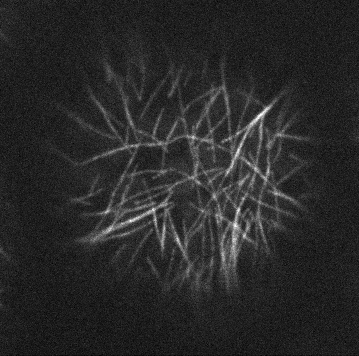
\includegraphics[height=2.2in]{benchImages/AVG-SPINNING-DISK-MARCHANTIA.png}
        \caption{Imagen de Microt\'ubulos}
        \label{fig:SpinningMarchantia-og}
    \end{subfigure}
    ~ 
    \begin{subfigure}[t]{0.49\textwidth}
        \centering
        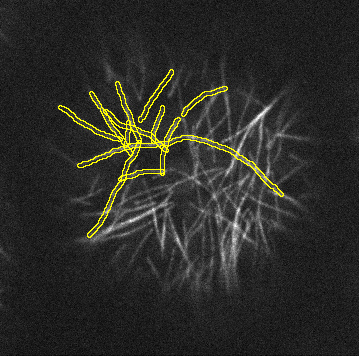
\includegraphics[height=2.2in]{benchImages/SPINNING-DISK-MARCHANTIA-rois-unlabeled.png}
        \caption{Filamentos manualmente individualizados por un experto}
        \label{fig:SpinningMarchantia-gt}
    \end{subfigure}
    \vskip\baselineskip
    \begin{subfigure}[t]{0.49\textwidth}
        \centering
        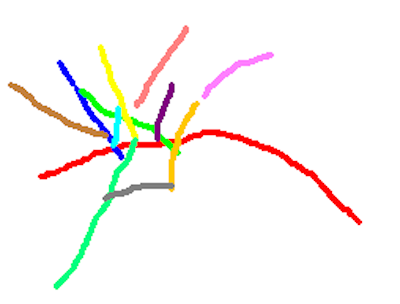
\includegraphics[height=2.2in]{benchImages/50-ROIs-Spinning-Marchantia-solved-rot-unlabeled.png}
        \caption{Codificaci\'on por color de la individualizaci\'on manual}
        \label{fig:SpinningMarchantia-indivManual}
    \end{subfigure}
    ~
    \begin{subfigure}[t]{0.49\textwidth}
        \centering
        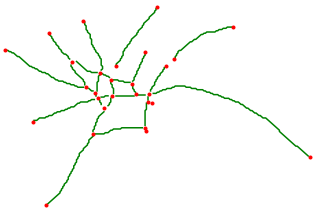
\includegraphics[height=2.2in]{benchImages/50-ROIs-Spinning-Marchantia-graph-og.png}
        \caption{Grafo que representa la red de microt\'ubulos manualmente identificada}
        \label{fig:SpinningMarchantia-graph}
    \end{subfigure}
    \caption{Individualizaci\'on manual de microt\'ubulos. a) Imagen 6 de un stack de 301 cuadros de {\it Arabidopsis Marchantia}. b) Individualizaci\'on manual c) Representaci\'on mediante colores de los diferentes microt\'ubulos. d) Grafo de 29 aristas extra\'ido a partir de la individualizaci\'on manual, que es el dato de entrada para los algoritmos comparados.}
    \label{fig:SpinningMarchantia}
\end{figure*}



%field3t02Bcell-filtered1
\begin{figure*}[h!]
    \centering
    \begin{subfigure}[t]{0.49\textwidth}
        \centering
        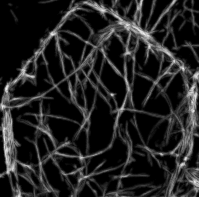
\includegraphics[height=2.2in]{benchImages/field3-t0-2cellBcrop-filtered-1.png}
        \caption{Imagen de Microt\'ubulos}
        \label{fig:field3t0filtered1-og}
    \end{subfigure}
    ~ 
    \begin{subfigure}[t]{0.49\textwidth}
        \centering
        \includegraphics[height=2.2in]{benchImages/field3-t0-2cellBcrop-filtered-1-rois.png}
        \caption{Filamentos manualmente individualizados por un experto}
        \label{fig:field3t0filtered1-gt}
    \end{subfigure}
    \vskip\baselineskip
    \begin{subfigure}[t]{0.49\textwidth}
        \centering
        \includegraphics[height=2.2in]{benchImages/field3-t0-2cellBcrop-filtered-inverted-colorCoded.png}
        \caption{Codificaci\'on por color de la individualizaci\'on manual}
        \label{fig:field3t0filtered1-indivManual}
    \end{subfigure}
    ~
    \begin{subfigure}[t]{0.49\textwidth}
        \centering
        \includegraphics[height=2.2in]{benchImages/field3-t0-2cellBcrop-filtered-graph-thick.png}
        \caption{Grafo extra\'ido a partir de la individualizaci\'on manual que es el dato de entrada para los algoritmos comparados.}
        \label{fig:field3t0filtered1-graph}
    \end{subfigure}
    \caption{Individualizaci\'on manual de microt\'ubulos. a) Imagen de {\it Arabidopsis Marchantia} obtenida al realizar la proyecci\'on del eje Z bajo el criterio de promedio de p\'ixeles. b) \'Areas de inter\'es de la individualizaci\'on manual c) Representaci\'on mediante colores de los diferentes microt\'ubulos. d) Grafo de 40 aristas utilizado en la individualizaci\'on autom\'atica de filamentos.}
    \label{fig:field3t0filtered1}
\end{figure*}



%field3t02Bcell-filtered2
\begin{figure*}[h!]
    \centering
    \begin{subfigure}[t]{0.49\textwidth}
        \centering
        \includegraphics[height=2.2in]{benchImages/field3-t0-2cellBcrop-filtered-2.png}
        \caption{Imagen de Microt\'ubulos}
        \label{fig:field3t0filtered2-og}
    \end{subfigure}
    ~ 
    \begin{subfigure}[t]{0.49\textwidth}
        \centering
        \includegraphics[height=2.2in]{benchImages/field3-t0-2cellBcrop-filtered-2-rois.png}
        \caption{Filamentos manualmente individualizados por un experto}
        \label{fig:field3t0filtered2-gt}
    \end{subfigure}
    \vskip\baselineskip
    \begin{subfigure}[t]{0.49\textwidth}
        \centering
        \includegraphics[height=2.2in]{benchImages/field3-t0-2cellBcrop-filtered-2-inverted-colorCoded.png}
        \caption{Codificaci\'on por color de la individualizaci\'on manual}
        \label{fig:field3t0filtered2-indivManual}
    \end{subfigure}
    ~
    \begin{subfigure}[t]{0.49\textwidth}
        \centering
        \includegraphics[height=2.2in]{benchImages/field3-t0-2cellBcrop-filtered-2-graph-thick.png}
        \caption{Grafo base para la individualizaci\'on automatizada de filamentos.}
        \label{fig:field3t0filtered2-graph}
    \end{subfigure}
    \caption{Individualizaci\'on manual de microt\'ubulos. a) Imagen de {\it Arabidopsis Marchantia} obtenida al realizar la proyecci\'on del eje Z bajo el criterio de promedio de p\'ixeles. b) \'Areas de inter\'es de la individualizaci\'on manual c) Representaci\'on mediante colores de los diferentes microt\'ubulos. d) Grafo de 7 aristas extra\'ido a partir de la individualizaci\'on manual.}
    \label{fig:field3t0filtered2}
\end{figure*}

%Porta6-4a1
\begin{figure*}[h!]
    \centering
    \begin{subfigure}[t]{0.49\textwidth}
        \centering
        \includegraphics[height=2.2in]{benchImages/grupo3-Porta6-4a1-MAX-cleaned.png}
        \caption{Imagen de una neurona}
        \label{fig:Porta6-4a1-og}
    \end{subfigure}
    ~ 
    \begin{subfigure}[t]{0.49\textwidth}
        \centering
        \includegraphics[height=2.2in]{benchImages/grupo3-Porta6-4a1-MAX-cleaned-colorCoded.png}
        \caption{Filamentos manualmente individualizados por un experto}
        \label{fig:Porta6-4a1-gt}
    \end{subfigure}
\vskip\baselineskip
    \begin{subfigure}[t]{0.5\textwidth}
        \centering
        \includegraphics[height=2in]{benchImages/grupo3-Porta6-4a1-MAX-cleaned-graph-thick.png}
        \caption{Grafo base para la individualizaci\'on automatizada de filamentos.}
        \label{fig:Porta6-4a1-graph}
    \end{subfigure}
    \caption{Individualizaci\'on manual de una neurona. a) Imagen de ... obtenida al realizar la proyecci\'on del eje Z bajo el criterio de valor m\'aximo de p\'ixeles. b) Representaci\'on mediante colores de los filamentos de la neurona, representando el ax\'on y las dendritas. d) Grafo de X aristas extra\'ido a partir de la individualizaci\'on manual.}
    \label{fig:Porta6-4a1}
\end{figure*}

%Porta10-5b
\begin{figure*}[h!]
    \centering
    \begin{subfigure}[t]{0.49\textwidth}
        \centering
        \includegraphics[height=1.9in]{benchImages/grupo1-Porta10-5b-AVG-partialCleaned.png}
        \caption{Imagen de una neurona}
        \label{fig:Porta10-5b-og}
    \end{subfigure}
    ~ 
    \begin{subfigure}[t]{0.49\textwidth}
        \centering
        \includegraphics[height=1.9in]{benchImages/grupo1-Porta10-5b-AVG-partialCleaned-colorCoded.png}
        \caption{Filamentos manualmente individualizados por un experto}
        \label{fig:Porta10-5b-gt}
    \end{subfigure}
    \vskip\baselineskip
    \begin{subfigure}[t]{0.5\textwidth}
        \centering
        \includegraphics[height=2in]{benchImages/grupo1-Porta10-5b-AVG_partialCleaned-graph-thick.png}
        \caption{Grafo base para la individualizaci\'on automatizada de filamentos.}
        \label{fig:Porta10-5b-graph}
    \end{subfigure}
    \caption{Individualizaci\'on manual de una neurona. a) Imagen de ... obtenida al realizar la proyecci\'on del eje Z bajo el criterio de valor m\'aximo de p\'ixeles. b) Representaci\'on mediante colores de los filamentos de la neurona, representando el ax\'on y las dendritas. d) Grafo de X aristas extra\'ido a partir de la individualizaci\'on manual.}
    \label{fig:Porta10-5b}
\end{figure*}


%Porta18-3a1
\begin{figure*}[h!]
    \centering
    \begin{subfigure}[t]{0.49\textwidth}
        \centering
        \includegraphics[height=1.9in]{benchImages/grupo2-Porta18-3a1-AVG-cleaned.png}
        \caption{Imagen de una neurona}
        \label{fig:Porta18-3a1-og}
    \end{subfigure}
    ~ 
    \begin{subfigure}[t]{0.49\textwidth}
        \centering
        \includegraphics[height=1.9in]{benchImages/grupo2-Porta18-3a1-AVG-cleaned-colorCoded.png}
        \caption{Filamentos manualmente individualizados por un experto}
        \label{fig:Porta18-3a1-gt}
    \end{subfigure}
    \vskip\baselineskip
    \begin{subfigure}[t]{0.5\textwidth}
        \centering
        \includegraphics[height=2in]{benchImages/grupo2-Porta18-3a1-AVG-cleaned-graph-thick.png}
        \caption{Grafo base para la individualizaci\'on automatizada de filamentos.}
        \label{fig:Porta18-3a1-graph}
    \end{subfigure}
    \caption{Individualizaci\'on manual de una neurona. a) Imagen de ... obtenida al realizar la proyecci\'on del eje Z bajo el criterio de valor m\'aximo de p\'ixeles. b) Representaci\'on mediante colores de los filamentos de la neurona, representando el ax\'on y las dendritas. d) Grafo de X aristas extra\'ido a partir de la individualizaci\'on manual.}
    \label{fig:Porta18-3a1}
\end{figure*}
\chapter{Resultados}
\label{chap:res}

Como se indica en el secci\'on \ref{sec:genGrafFromImage}, la obtenci\'on de un grafo a partir de una imagen es un proceso complejo. Las im\'agenes analizadas en este trabajo son aquellas en las que fue posible realizar el procedimiento de esqueletonizaci\'on, obteniendo un resultado que manten\'ia la topolog\'ia de la estructura original. Lo anterior no es un resultado que pueda garantizarse para toda imagen. 


%Los resultados que se presentan a continuaci\'on se separan entre tablas y figuras. Las tablas de resultados se encuentran dividas en 2 secciones dado el n\'umero de columnas. La primera secci\'on agrupa las m\'etricas y medidas indicadas en la secci\'on \ref{sec:metricasymedidas}, mientras que la segunda secci\'on muestra los porcentajes de cobertura y correctitud de los filamentos propuestos con respecto a la individualizaci\'on manual propuesta por un experto. Es necesario especificar que los porcentajes que se indican en la columna `` \% Cobertura de Aristas'' reflejan una condici\'on que no es una restricci\'on estricta del modelo o del algoritmo propuesto, a diferencia de DeFiNe, donde si se fuerza la cobertura de cada arista del grafo.


%En cuanto a las figuras, el enfoque se dirige a presentar los resultados de DeFiNe y del algoritmo propuesto, con \'enfasis en los filamentos correctamente encontrados por uno de los algoritmos que el otro no haya podido individualizar. Cabe aclarar que el resultado gr\'afico al ejecutar DeFiNe realiza una rotaci\'on de 90\textdegree en sentido contrarreloj adem\'as de invertir el eje vertical. Ambas modificaciones han sido corregidas con el prop\'osito de comparar los resultados entre DeFiNe, el algoritmo propuesto y la individualizaci\'on de filamentos realizada por el experto.

Como se indica en la secci\'on \ref{sec:SynthImgMethod}, las mediciones del algoritmo propuesto pueden utilizar los par\'ametros predefinidos para distintos tipos de c\'elula, as\'i como modificar algunos de estos manualmente. Adem\'as, el c\'alculo de cada evaluaci\'on del algoritmo propuesto consiste en el promedio de 5 iteraciones, cada una con una semilla diferente.

El detalle de cada iteraci\'on, en conjunto con el c\'odigo y otros elementos necesarios para replicar estos resultados se encuentra en el \href{https://gitlab.com/LeoXDXp/graph-crawler}{repositorio git de esta tesis}. Parte de este detalle se incluye tambi\'en en el anexo \ref{chap:apendice}.
Las ejecuciones de DeFiNe y el algoritmo propuesto fueron realizadas en un computador con un procesador {\tt Intel i5-7200U} de 4 n\'ucleos, 8GB de RAM y un disco de estado s\'olido, bajo el sistema operativo {\tt Fedora 31}.

\section{Extracci\'on de un grafo desde una imagen}
\label{sec:graphImageExtraction}
La obtenci\'on de un grafo y la asociaci\'on de propiedades a sus nodos o aristas constituye el paso previo a la individualizaci\'on autom\'atica de filamentos. De acuerdo a lo descrito en la secci\'on \ref{subsec:infoLossSkel}, existen diversas formas para realizar este procedimiento. Para el caso de DeFiNe, sus autores indican que se preprocesa la imagen en escala de grises para resaltar las estructuras alargadas que debiesen ser filamentos, mediante un filtro de {\it veselness} y un umbral de mediana adaptativa. El paso siguiente consiste en realizar la esqueletonizaci\'on de la imagen, para luego construir un grafo en el que se asigna un peso a las aristas. 
Para obtener el peso de las aristas, se le aplica un filtro gaussiano a la imagen original en escala de grises, para luego promediar la intensidad a lo largo de cada arista.

% solo esta disponible el archivo GML para la imagen sintetica 1. No estan disponibles las imagenes base,

Una replica exacta de los pasos de aquel procedimiento no puede ser realizada, debido a que no se se\~nala el tama\~no del filtro gaussiano. Otro aspecto que dificulta una comparaci\'on directa es que DeFiNe no considera la curvatura de las aristas, sino que solo las representa como lineas rectas mediante la conexión punto a punto entre los nodos. Adicionalmente, no se encontraron las im\'agenes originales utilizadas en aquella investigaci\'on. Lo anterior implica que la solo se pudo realizar una comparaci\'on precisa entre DeFiNe y el algoritmo propuesto, utilizando el \'unico ejemplo que trae DeFiNe, que corresponde al grafo ponderado con el que se realiza la individualizaci\'on de filamentos de la Figura 1b de aquella investigaci\'on, a partir de la cual se extrae una secci\'on, representada en la Figura \ref{fig:synth-Define-1b}.


En los otros casos donde se utiliza DeFiNe para obtener una individualizaci\'on de filamentos, se extrae el grafo necesario utilizando la herramienta {\it sknw}, la que pondera cada arista con su respectivo largo, el cual s\'i considera la curvatura. Este enfoque es compatible con lo que se presenta en \cite{breuer2015define}, ya que se indica que el m\'etodo utilizado por DeFiNe sirve para cualquier red ponderada extra\'ida a partir de una imagen.


\section{Im\'agenes Sint\'eticas}

%Resultados Synth QFS
Para la individualizaci\'on de los filamentos sint\'eticos en la Figura \ref{fig:synth-QFS-7} se utilizan los par\'ametros predefinidos en la opci\'on de microt\'ubulos de planta, ya que la figura refleja similitudes con este tipo de filamentos.
Los resultados se indican en la Tabla \ref{tab:synth-QFS-7-Results}, observ\'andose que DeFiNe logra 4 de 6 individualizaciones al utilizar 30\textdegree, mientras que con 60\textdegree obtiene 3 de 6 filamentos correctos. Este \'ultimo resultado es el mismo que se obtiene al promediar todas las iteraciones del algoritmo propuesto con los par\'ametros de microt\'ubulo de planta, al que se denomina Prueba 1.

Debido a que el comportamiento de los filamentos sint\'eticos es m\'as simple que el los microt\'ubulos de planta, se realizaron pruebas utilizando como base los par\'ametros para filamentos sint\'eticos, modificando el \'angulo a 20\textdegree y aplicando la heur\'istica de asignaci\'on inicial parcialmente, defini\'endose como Prueba 2. Esto \'ultimo se debe a que en filamentos sint\'eticos no se requiere de explorar diversos puntos de partida como si sucede en una imagen real de filamentos. Estos par\'ametros permiten encontrar 4 de 6 filamentos. La comparaci\'on entre los filamentos propuestos por cada m\'etodo y los correctamente identificados se observa en la Figura \ref{fig:Synth-QIFS-Result}.


En este caso de filamentos sint\'eticos, el filamento azul observable en la Figura \ref{fig:synth-QFS-7-gt}, corresponde a una sola arista del grafo (Figura \ref{fig:synth-QFS-7-graph}), por lo que tambi\'en en todas las pruebas con DeFiNe y con el algoritmo propuesto se obtiene para ese filamento un calce no exacto. Este calce no exacto no se considera una respuesta correcta, pero representa una situaci\'on que puede suceder en im\'agenes reales, en las que puede representar el nacimiento de un filamento a partir de otro existente, como sucede en neuronas o microt\'ubulos. 
%En situaciones como esta, el uso de un criterio compuesto es necesario, dado que el s\'olo uso de \'angulo o de intensidad no es una caracter\'istica suficiente, existiendo una dependencia de la informaci\'on a priori de la c\'elula observada. Caso de MT con 45\textdegree y que eso se encuentra en el limite de la neurona
Luego, la sobre-representaci\'on del filamento correcto en la figura (filamento azul) sucede al agregar una arista del filamento vecino, de color celeste.


Ambas ejecuciones de DeFiNe, as\'i como todas las ejecuciones del algoritmo propuesto logran asignar cada arista a al menos un camino que representa un filamento. Este comportamiento es obligatorio para el m\'etodo de DeFiNe pero no para el algoritmo propuesto.

%Con respecto a los indicadores, {\it Precision} y {\it Recall} ...
%el mejor resultado de la prueba 2 obtiene un recall 1 ya que adem\'as de presentar 4 filamentos correctos con respecto al criterio del experto, se le considera tambi\'en el filamento en sobre-asignaci\'on.

% pq hay una penalizacion en todos los indicadores a pesar tener lo mismo q define 60
%%%% Como explicar VI, Rand y Jaccard, y los otros numeros

\begin{table}[h]
    \centering
    \begin{tabular}{|l|c|c|c|c|c|c|c|c|c|}
    \hline
          Algoritmo & VI & Rand & Jaccard & Precision & Recall & F1 & C/P & C/GT & Tiempo[s] \\ \hline
         DeFiNe 30\textdegree & 0.7958 & 0.8461 & 0.4 & 0.7272 & 0.4705 & 0.5714 & 4/6 & 4/6 & 2.3128 \\
         DeFiNe 60\textdegree & 0.9777 & 0.8636 & 0.4375 & 0.6363 & 0.5833 & 0.6086 & 3/5 & 3/6 & 2.3380\\
         \multirow{2}{1.9cm}{Promedio Prueba 1}
          &&&&&&&&&\\  
        & 1.6360 & 0.7646 & 0.2484 & 0.5142 & 0.3289 & 0.3919 & 3/6.2 & 3/6 & 0.3569\\
         \multirow{2}{1.9cm}{Mejor \\Prueba 1}
         &&&&&&&&&\\
         & 1 & 0.8461 & 0.4	& 0.5714 & 0.5714 & 0.5714 & 3/5 & 3/6 & 0.3135 \\
         \multirow{2}{1.9cm}{Promedio Prueba 2}
         &&&&&&&&&\\
         & 0.7090 & 0.8636 &0.475 &0.6892 &	0.5789 & 0.6230 & 4/5.8 & 4/6 & 0.2908\\
         \multirow{2}{1.9cm}{Mejor \\Prueba 2}
         &&&&&&&&&\\
         & 0.2727 & 0.9777 & 0.875 & 0.875 & 1 & 0.9333 & 4/5 & 4/6 & 0.3073\\
         \hline
    \end{tabular}
    \caption{M\'etricas y medidas en la individualizaci\'on de filamentos de la Figura \ref{fig:synth-QFS-7}. El valor m\'aximo de VI es de 2.397895, debido a que el n\'umero de aristas es 11. El n\'umero de filamentos correctos es 6. La columna C/P refleja el n\'umero de filamentos correctos con respecto a los propuestos por cada m\'etodo, mientras que la columna C/GT indica la relaci\'on entre los filamentos correctamente individualizados por el m\'etodo y el criterio del experto.}
    \label{tab:synth-QFS-7-Results}
\end{table}


\begin{figure*}[h!]
    \centering
    \hspace{0.2cm}
    \begin{subfigure}[t]{0.48\textwidth}
        \centering
        \includegraphics[height=1.5in]{resultImages/QFS7-DeFiNeExactMatch-30.png}
        \caption{Representaci\'on del resultado de DeFiNe con \'angulo de 30\textdegree, con 4 filamentos correctamente individualizados, identificados con colores.}
        \label{fig:SpinningMarchantiaResults-define30Exact}
    \end{subfigure}
    \begin{subfigure}[t]{0.48\textwidth}
        \centering
        \includegraphics[height=1.5in]{resultImages/QFS7-DeFiNeExactMatch-60.png}
        \caption{Representaci\'on del resultado de DeFiNe con \'angulo de 60\textdegree, con 3 filamentos correctamente individualizados, identificados con colores.}
        \label{fig:SpinningMarchantiaResults-define60Exact}
    \end{subfigure}
    \vskip\baselineskip
    \begin{subfigure}[t]{0.47\textwidth}
        \centering
        \includegraphics[scale=0.13]{resultImages/Synth-QuantitativeIFS-Fig7-phil-s1271-v05-exactMatch-antLabeled.png}
        \caption{Filamentos individualizados con colores a partir de la mejor iteraci\'on del algoritmo propuesto con la configuraci\'on definida como Prueba 1.}
        \label{fig:SynthQFS7-Individualizacion-BestP1}
    \end{subfigure}
    \hspace{0.2cm}
    \begin{subfigure}[t]{0.47\textwidth}
        \centering
        \includegraphics[scale=0.13]{resultImages/Synth-QuantitativeIFS-Fig7-phil-s1271-v056-exactMatch-antLabeled.png}
        \caption{Filamentos individualizados con colores a partir de la mejor iteraci\'on del algoritmo propuesto con la configuraci\'on definida como Prueba 2.}
        \label{fig:SynthQFS7-Individualizacion-BestP2}
    \end{subfigure}
        
    \caption{Individualizaci\'on de filamentos correctos respecto a la evaluaci\'on de un experto para la Figura \ref{fig:synth-QFS-7}. El algoritmo propuesto individualiza correctamente 3 filamentos con la configuraci\'on para microt\'ubulos de planta, mejorando a 4 filamentos con una configuraci\'on m\'as simple.}
    \label{fig:Synth-QIFS-Result}
\end{figure*}

%\clearpage
%\newpage
%%%%%%%%%% End synth QFS 7 - Begin Synth DeFiNe 1b %%%%%%%



%Resultados Synth Define

Como se menciona en la secci\'on \ref{sec:graphImageExtraction}, la Figura \ref{fig:synth-Define-1b} corresponde a una parte de la Figura 1b en \cite{breuer2015define}, siendo la \'unica imagen para la que se dispone de un grafo ponderado seg\'un el criterio de los autores de DeFiNe. As\'i, se asume que aquel es el resultado \'optimo, en el que se individualizan correctamente los 5 filamentos. Una diferencia del grafo utilizado en la evaluaci\'on del algoritmo propuesto, con respecto al grafo que permite individualizar aquellos 5 filamentos, radica en que el utilizado con el algoritmo propuesto divide 1 de los 5 filamentos en 2, generando 6 filamentos en total. Es por ello, que las dem\'as evaluaciones con respecto a la Figura \ref{fig:synth-Define-1b} indican 6 filamentos como {\it ground truth}.


En la evaluaci\'on del algoritmo propuesto utilizando los par\'ametros definidos para microt\'ubulos de plantas, se obtienen 3 individualizaciones correctas de los 5 filamentos que corresponden al {\it ground truth}. En esta evaluaci\'on, denominada Prueba 3, s\'olo 1 filamento individualizado se encuentra dentro del grupo de filamentos que se intersectan y sobreponen entre s\'i. Es posible atribuir esto a la curvatura de algunos de los filamentos sint\'eticos, la que es mayor a la que se espera de un microt\'ubulos de planta. Para complementar la evaluaci\'on, se realiza la Prueba 4 en la que se elige el tipo de c\'elula sint\'etica, modificando el factor $Max\_Axial\_Displacement$ a 2, asociado a la curvatura que presenta la figura, y no utilizando la heur\'istica de asignaci\'on inicial completa, dado que no existen casos complejos de nacimiento de filamentos a partir de otros como en filamentos reales.

As\'i, la Prueba 4 permite encontrar un filamento adicional, y a su vez, es capaz de encontrar el filamento naranja de la individualizaci\'on manual del experto, indicado en la Figura \ref{fig:synth-Define-1b-graph-gt}, pero es descartado por no respetar el criterio de la magnitud de desplazamiento entre segmentos. El comportamiento del filamento naranja en el {\it ground truth} realiza un cambio de sentido en sus curvaturas, adem\'as de que estas son bastante pronunciadas, lo que no es un comportamiento esperado en los filamentos estudiados durante esta investigaci\'on. Los resultados se presentan en la Tabla \ref{tab:synth-Define-1b}.


%Con respecto a las medidas, se obtiene un alto valor de VI, lo que es atribuible a que en este caso existen varios casos de solapamiento entre filamentos, mientras que con la configuraci\'on para microt\'ubulos de planta, los \'indices {\it Rand} y {\it Jaccard} son disimiles entre s\'i, con enf\'asis en que el \'indice {\it Jaccard} arroja un resultado muy cercano a 0.


\begin{table}[h]
    \centering
    \begin{tabular}{|l|c|c|c|c|c|c|c|c|c|}
    \hline
          Algoritmo & VI & Rand & Jaccard & Precision & Recall & F1 & C/P & C/GT & Tiempo[s] \\ \hline
         DeFiNe 30\textdegree & 1.7159 & 0.7792 & 0.1355 & 0.3333 & 0.1860 & 0.2388 & 2/11 & 2/5 & 2.8275 \\
         DeFiNe 60\textdegree & 2.45 & 0.6719 & 0.1388 & 0.238 & 0.25 & 0.2439 & 2/7 & 2/5 & 3.6597\\
         \multirow{2}{1.9cm}{Promedio Prueba 3}
          &&&&&&&&&\\  
        & 2.2296 & 0.7276 & 0.1806 & 0.3418 & 0.2775 & 0.3056 & 3/9.2 & 3/6 & 0.3569\\
         \multirow{2}{1.9cm}{Mejor \\Prueba 3}
         &&&&&&&&&\\
         & 1.9171 & 0.7446 & 0.1862 & 0.3518 & 0.2835 & 0.314 & 3/9 & 3/6 & 0.3135 \\
         \multirow{2}{1.9cm}{Promedio Prueba 4}
         &&&&&&&&&\\
         & 2.5878 & 0.7275 & 0.1673 & 0.3257 & 0.2578 & 0.2863 & 4/8.6 & 4/5 & 0.325378\\
         \multirow{2}{1.9cm}{Mejor \\Prueba 4}
         &&&&&&&&&\\
         & 2.2728 & 0.7176 & 0.1923 & 0.3361 & 0.31 & 0.3225 & 4/9 & 4/6 & 0.3299\\
         \hline
    \end{tabular}
    \caption{Individualizaci\'on de filamentos para la Figura \ref{fig:synth-Define-1b}.  El valor m\'aximo de VI para este caso es 2.83321, dado que el grafo esta compuesto por 17 aristas. El n\'umero de filamentos definidos manualmente por un experto es 5. La columna C/P refleja el n\'umero de filamentos correctos con respecto a los propuestos por cada m\'etodo, mientras que la columna C/GT indica la relaci\'on entre los filamentos correctamente individualizados por el m\'etodo y el criterio del experto.}
    \label{tab:synth-Define-1b}
\end{table}

\begin{figure*}[h!]
    \centering
    \begin{subfigure}[t]{0.49\textwidth}
        \centering
        \includegraphics[scale=0.1]{resultImages/defineFig1b-DeFiNeExactMatch-30.png}
        \caption{Representaci\'on del resultado obtenido a trav\'es de DeFiNe con 30\textdegree, logrando 2 filamentos correctamente individualizados, identificados con colores.}
        \label{fig:SynthDefine-Results-define30Exact}
    \end{subfigure}
    ~
    \begin{subfigure}[t]{0.49\textwidth}
        \centering
        \includegraphics[scale=0.1]{resultImages/defineFig1b-DeFiNeExactMatch-60.png}
        \caption{Representaci\'on del resultado obtenido a trav\'es de DeFiNe con 60\textdegree, logrando 2 filamentos correctamente individualizados, identificados con colores.}
        \label{fig:SynthDefine-Results-define60Exact}
    \end{subfigure}
    \vskip\baselineskip
    
    \begin{subfigure}[t]{0.49\textwidth}
        \centering
        \includegraphics[scale=0.11]{resultImages/define-weighted-4-phil-s0-v05-exactMatch-antLabeled.png}
        \caption{3 filamentos correctamente individualizados por el algoritmo propuesto con la configuraci\'on definida como Prueba 3.}
        \label{fig:SynthDefine-Individualizacion-BestP1}
    \end{subfigure}
    ~
    \begin{subfigure}[t]{0.49\textwidth}
        \centering
        \includegraphics[scale=0.11]{resultImages/define-weighted-4-phil-s3389-v056-exactMatch-antLabeled.png}
        \caption{4 filamentos correctamente individualizados por el algoritmo propuesto con la configuraci\'on definida como Prueba 4.}
        \label{fig:SynthDefine-Individualizacion-BestP2}
    \end{subfigure}
    
    \caption{Resultados de la individualizaci\'on de filamentos para la Figura \ref{fig:synth-Define-1b}, obtenidas mediante DeFiNe y el algoritmo propuesto, con diferentes par\'ametros. El algoritmo propuesto encuentra m\'as filamentos que los que se encuentran en las pruebas con DeFiNe. Sin embargo se aleja del comportamiento \'optimo indicado en \cite{breuer2015define}. Esta diferencia puede atribuirse a la excesiva curvatura de los filamentos sint\'eticos.}
    \label{fig:SynthDefine-Result}
\end{figure*}
\clearpage
\newpage
%%%%%%%%%% End Synth DeFiNe 1b %%%%%%%

\section{Im\'agenes Reales}

%recordar que define es base de BFS-Overlap-pairwise-total-
% recordarr que son 5 iteraciones y se estan promediando los resultados, conectar con la columna cobertura 
En esta secci\'on se muestran los resultados de la individualizaci\'on de filamentos para 2 tipos de c\'elulas, los microt\'ubulos existentes en la planta {\it Arabidopsis Marchantia}, y las dendritas en neuronas de rat\'on. Para cada tipo de c\'elulas existen 3 im\'agenes reales con las que se cuenta con la respectiva individualizaci\'on manual realizada por un experto. Se realizan pruebas utilizando las configuraciones predefinidas para estas c\'elulas en base a la informaci\'on recabada ante expertos.

\subsection{Microt\'ubulos de planta}
\label{subsec:mtTest}

%Valor m\'ax de VI para \ref{tab:SpinningMarchantiaResults1} es 3.4965.
%N\'umero de filamentos en el {\it Ground Truth} de la figura SpinningMarchanria es 12.
%Define y Phil presentan una propuesta de filamento para el ....

La primera evaluaci\'on corresponde a la muestra MT-A, indicada en la figura \ref{fig:SpinningMarchantia}, la que corresponde a una individualizaci\'on manual realizada por un experto a partir de una red de microt\'ubulos en la planta {\it Arabidopsis Marchantia}. La evaluaci\'on llevada a cabo mediante el algoritmo propuesto con los par\'ametros predefinidos para microt\'ubulos de planta se denomina Prueba 5, y sus resultados, en conjunto con los resultados de DeFiNe se presentan en la Tabla \ref{tab:SpinningMarchantiaResults}.

De los 12 filamentos identificados por un experto, DeFiNe con un \'angulo de 30\textdegree~ individualiza 8 correctamente, mientras que con un \'angulo de 60\textdegree~ logra 3 individualizaciones correctas. Por su parte, el resultado del algoritmo propuesto con los par\'ametros predefinidos, indica que 4 de 5 pruebas individualizan al menos 7 filamentos correctamente, teniendo un caso donde se logran 8 aciertos. Lo anterior se refleja en la Figura \ref{fig:SpinningMarchantiaResults}. Se debe destacar que en 3 de las 4 pruebas que no logran encontrar el filamento adicional, existe una sobre-representaci\'on de aquel filamento ya que se le asigna una arista adicional, lo que lleva a no considerarlo como una respuesta correcta. 


Otros aspecto de estos resultados es que todas las evaluaciones logran una cobertura total de las aristas en sus propuestas de individualizaci\'on. Por su parte, las iteraciones durante la Prueba 5 para el algoritmo propuesto, muestran estabilidad en el resultado para los par\'ametros predefinidos, logrando obtener la mayor\'ia de los filamentos que obtiene DeFiNe en sus 2 evaluaciones.

\begin{table}[h]
    \centering
    \begin{tabular}{|l|c|c|c|c|c|c|c|c|c|}
    \hline
          Algoritmo & VI & Rand & Jaccard & Precision & Recall & F1 & C/P & C/GT & Tiempo[s] \\ \hline
         DeFiNe 30\textdegree & 1.1033 & 0.9242 & 0.3650 & 0.6571 & 0.4509  & 0.5348 & 8/16 & 8/12 & 4.1087 \\
         DeFiNe 60\textdegree & 2.6025 & 0.8539 & 0.1401 & 0.2830 & 0.2173 & 0.2459 & 3/12 & 3/12 & 3.6597 \\
         \multirow{2}{1.9cm}{Promedio Prueba 5}
          &&&&&&&&&\\  
        & 2.1283 & 0.8658 & 0.2406 & 0.4404 & 0.3465 & 0.3878 & 7.2/12.4 & 7.2/12 & 0.3569\\
         \multirow{2}{1.9cm}{Mejor \\Prueba 5}
         &&&&&&&&&\\
         & 1.9791 & 0.8696 & 0.25 & 0.4574 & 0.3553 & 0.4 & 8/13 & 8/12 & 0.3135 \\
         \hline
    \end{tabular}
    \caption{Resultados de individualizaci\'on de filamentos para la muestra MT-A en la Figura \ref{fig:SpinningMarchantia}. El valor m\'aximo de VI en este caso es de 3.3672, ya que el tama\~no del {\it data set} es de 29 aristas. El n\'umero de filamentos en el {\it ground truth} es 12.}
    \label{tab:SpinningMarchantiaResults}
\end{table}


\begin{figure*}[h!]
    \centering
    \begin{subfigure}[t]{0.49\textwidth}
        \centering
        \includegraphics[scale=0.6]{resultImages/SpinningMarchantia-Define30.png}
        \caption{Individualizaci\'on obtenida mediante DeFiNe con un \'angulo de 30\textdegree .}
        \label{fig:SpinningMarchantiaResults-define30}
    \end{subfigure}%
    ~ 
    \begin{subfigure}[t]{0.49\textwidth}
        \centering
        \includegraphics[height=1.3in]{resultImages/50-ROIs-Spinning-Marchantia-DeFiNeExactMatch-30.png}
        \caption{Representaci\'on de los filamentos correctamente individualizados en (a), identificados con colores.}
        \label{fig:SpinningMarchantiaResults-define30Exact}
    \end{subfigure}
    \vskip\baselineskip
    
    \begin{subfigure}[t]{0.49\textwidth}
        \centering
        \includegraphics[scale=0.6]{resultImages/SpinningMarchantia-Define60.png}
        \caption{Individualizaci\'on obtenida mediante DeFiNe con un \'angulo de 60\textdegree .}
        \label{fig:SpinningMarchantiaResults-define60}
    \end{subfigure}
    ~ 
    \begin{subfigure}[t]{0.49\textwidth}
        \centering
        \includegraphics[height=1.3in]{resultImages/50-ROIs-Spinning-Marchantia-DeFiNeExactMatch-60.png}
        \caption{Representaci\'on de los filamentos correctamente individualizados en (c), identificados con colores.}
        \label{fig:SpinningMarchantiaResults-define60Exact}
    \end{subfigure}
    \vskip\baselineskip
    
    \begin{subfigure}[t]{0.49\textwidth}
        \centering
        \includegraphics[height=1.4in]{resultImages/50-ROIs-Spinning-Marchantia-phil-s0-v05-nobg-antLabeled.png}
        \caption{Mejor resultado de la individualizaci\'on de filamentos usando el algoritmo propuesto con la configuraci\'on para microt\'ubulos de planta.}
        \label{SpinningMarchantiaResults-bestPhil}
    \end{subfigure}
    ~
    \begin{subfigure}[t]{0.49\textwidth}
        \centering
        \includegraphics[height=1.4in]{resultImages/50-ROIs-Spinning-Marchantia-phil-s0-v05-exactMatch-antLabeled-thick.png}
        \caption{8 filamentos correctamente individualizados en base al resultado de (e).}
        \label{fig:SpinningMarchantiaResults-bestPhilExact}
    \end{subfigure}
    \vskip\baselineskip
    
    \begin{subfigure}[t]{0.49\textwidth}
        \centering
        \includegraphics[height=1.4in]{resultImages/50-ROIs-Spinning-Marchantia-phil-s10-v05-nobg-antLabeled.png}
        \caption{Resultado promedio de la individualizaci\'on de filamentos usando el algoritmo propuesto con la configuraci\'on para microt\'ubulos de planta.}
        \label{SpinningMarchantiaResults-worstPhil}
    \end{subfigure}
    ~ 
    \begin{subfigure}[t]{0.49\textwidth}
        \centering
        \includegraphics[height=1.4in]{resultImages/50-ROIs-Spinning-Marchantia-phil-s10-v05-exactMatch-antLabeled-thick.png}
        \caption{7 filamentos correctamente individualizados en base al resultado de (g).}
        \label{fig:SpinningMarchantiaResults-worstPhilExact}
    \end{subfigure}
    
    \caption{Filamentos propuestos y correctamente individualizados a partir la muestra MT-A en la Figura \ref{fig:SpinningMarchantia}, obtenidos mediante DeFiNe y el algoritmo propuesto con sus respectivos par\'ametros. Segmentos marcados en negro representan aristas no asignadas correctamente al filamento correspondiente en el {\it ground truth}, mientras que los filamentos correctamente identificados se encuentran identificados mediante colores.}
    \label{fig:SpinningMarchantiaResults}
\end{figure*}

\clearpage
\newpage


La segunda evaluaci\'on de microt\'ubulos de planta corresponde a la muestra MT-B, que se observa en la Figura \ref{fig:field3t0filtered1}, y cuya individualizaci\'on de filamentos usando el algoritmo propuesto se define como Prueba 6. En base a los resultados del algoritmo propuesto, los que individualizan correctamente 8 filamentos en promedio, se observa la necesidad de un rango de tolerancia para determinar si una soluci\'on propuesta corresponde a un filamento. Esto se debe a que el grafo que representa la red de filamentos es una representaci\'on discreta, de la que pueden aparecer aristas que forman \'angulos por sobre los umbrales definidos, llevando a descartar estas soluciones sin su completa evaluaci\'on.

Un aspecto a destacar del algoritmo propuesto, radica que 4 de las 5 iteraciones de la Prueba 6 encuentran 9 filamentos, proponiendo 15 filamentos en promedio, lo que es menor a ambas evaluaciones realizadas con DeFiNe. A su vez, el algoritmo propuesto muestra un mejor desempe\~no en su tiempo de ejecuci\'on, demostrando poder soportar grafos de mayor n\'umero de nodos y aristas.

\begin{table}[h]
    \centering
    \begin{tabular}{|l|c|c|c|c|c|c|c|c|c|}
    \hline
          Algoritmo & VI & Rand & Jaccard & Precision & Recall & F1 & C/P & C/GT & Tiempo[s] \\ \hline
         DeFiNe 30\textdegree & 1.8847 & 0.9065 & 0.1512 & 0.5142 & 0.1764 & 0.2627 & 5/23 & 5/12 & 5.0306 \\
         DeFiNe 60\textdegree & 2.0731 & 0.8576 & 0.2198 & 0.425 & 0.3127 & 0.3604 & 5/16 & 5/12 & 16.2042 \\
         \multirow{2}{1.9cm}{Promedio Prueba 6}
          &&&&&&&&&\\  
        & 2.6284 & 0.8683 & 0.2487 & 0.5079 & 0.3283 & 0.3976 & 8.8/15 & 8.8/12 & 0.9693\\
         \multirow{2}{1.9cm}{Mejor \\Prueba 6}
         &&&&&&&&&\\
         & 2.1620 & 0.8781 & 0.2958 & 0.5263 & 0.4032 & 0.4566 & 9/14 & 9/12 & 1.0342 \\
         \hline
    \end{tabular}
    \caption{Resultados de la individualizaci\'on de filamentos para la muestra MT-B (Figura \ref{fig:field3t0filtered1}). El valor m\'aximo de VI en este caso es de 3.6888, ya que el n\'umero de aristas en el grafo utilizado es 40. 12 son los filamentos definidos por un experto. El algoritmo propuesto presenta un comportamiento favorable, presentando un n\'umero de filamentos propuestos cercano a la cantidad de filamentos correctos.}
    \label{tab:field3t0filtered1}
\end{table}


\begin{figure*}[h!]
    \centering
    \begin{subfigure}[t]{0.49\textwidth}
        \centering
        \includegraphics[height=1.5in]{resultImages/field3-t0-2cellBcrop-filtered-DeFiNeExactMatch-30.png}
        \caption{Representaci\'on de los 5 filamentos correctamente individualizados por DeFiNe con 30\textdegree, identificados con colores}
        \label{fig:field3t0filtered1Results-define30Exact}
    \end{subfigure}
    ~ 
    \begin{subfigure}[t]{0.49\textwidth}
        \centering
        \includegraphics[height=1.5in]{resultImages/field3-t0-2cellBcrop-filtered-DeFiNeExactMatch-60.png}
        \caption{Representaci\'on de los 5 filamentos correctamente individualizados por DeFiNe con 60\textdegree, identificados con colores}
        \label{fig:field3t0filtered1Results-define60Exact}
    \end{subfigure}
    
    \vskip\baselineskip
    \begin{subfigure}[t]{0.49\textwidth}
        \centering
        \includegraphics[height=1.5in]{resultImages/field3-t0-2cellBcrop-filtered-phil-s0-v056-exactMatch-antLabeled.png}
        \caption{Resultado promedio de Prueba 6, con 8 filamentos correctamente individualizados, identificados con colores.}
        \label{field3t0filtered1Results-bestPhil}
    \end{subfigure}
    ~ 
    \begin{subfigure}[t]{0.49\textwidth}
        \centering
        \includegraphics[height=1.5in]{resultImages/field3-t0-2cellBcrop-filtered-phil-s10-v056-exactMatch-antLabeled.png}
        \caption{9 Filamentos correctamente individualizados a partir del mejor resultado del algoritmo propuesto para la Prueba 6, identificados con colores.}
        \label{fig:field3t0filtered1Results-bestPhilExact}
    \end{subfigure}
    
    \caption{Filamentos correctamente individualizados en la figura \ref{fig:field3t0filtered1} correspondiente a la muestra MT-B, mediante el DeFiNe y el algoritmo propuesto. Segmentos marcados en negro representan aristas no asignadas correctamente. El mejor resultado del algoritmo propuesto permite encontrar filamentos no encontrados en a) o b).}
    \label{fig:field3t0filtered1Results}
\end{figure*}
\clearpage
\newpage

%Valor m\'ax de VI para \ref{tab:field3t0filtered2} es 1.9459.
%N\'umero de filamentos en el {\it Ground Truth} de la figura field3t0 es 5.

La individualizaci\'on de filamentos para la Figura \ref{fig:field3t0filtered2}, que representa la muestra MT-C, entrega los mismos resultados al ejecutar tanto DeFiNe con 60\textdegree~ como el algoritmo propuesto con los par\'ametros predefinidos para microt\'bulos de planta. Esta \'ultima evaluaci\'on corresponde a la Prueba 7. Esto puede deberse a que la muestra MT-C es de mayor simplicidad que las muestras anteriores. Por su parte, la ejecuci\'on de DeFiNe con 30\textdegree~ individualiza correctamente 3 de 5 filamentos. Los resultados se indican en la Tabla \ref{tab:field3t0filtered2} y en l Figura \ref{fig:field3t0filtered2Results}.



El filamento faltante para el algoritmo propuesto corresponde a una sobre-asignaci\'on de aristas, similar a lo que ocurre en otras im\'agenes, llevando a no considerar aquella soluci\'on como un filamento valido. La posibilidad de sobre-asignar una arista a un filamento se condice con el comportamiento del algoritmo propuesto al favorecer la b\'usqueda de caminos/filamentos de mayor longitud que cumplan con el criterio de rectitud. Particularmente en este caso, un microt\'ubulo de planta puede corresponder a la fusi\'on de 2 microt\'ubulos en uno, denominado {\tt Zippering}, o al nacimiento de un microt\'ubulo a partir de uno existente, llamado {\tt Nucleaci\'on}. Ambas situaciones requieren de informaci\'on adicional para diferenciarlas, pudiendo usarse caracter\'isticas como el grosor de los segmentos de los filamentos involucrados en estas situaciones, as\'i como el \'angulo entre los segmentos de filamentos que se separan del segmento com\'un. La variaci\'on o continuidad del grosor y que el \'angulo mencionado se encuentre en un rango que var\'ia seg\'un el tipo de c\'elula son cr\'iticos para aclarar cual es el caso observado. 


%En relaci\'on al an\'alisis de las medidas y las m\'etricas en la tabla \ref{tab:field3t0filtered2}, se mantiene el empate entre DeFiNe-60\textdegree y Phil, con la \'unica diferencia en el tiempo de ejecuci\'on, favorable para Phil. 

\begin{table}[h]
    \centering
    \begin{tabular}{|l|c|c|c|c|c|c|c|c|c|}
    \hline
          Algoritmo & VI & Rand & Jaccard & Precision & Recall & F1 & C/P & C/GT & Tiempo[s] \\ \hline
         DeFiNe 30\textdegree & 0.5714 & 0.9047 & 0.3333 & 0.5 & 0.5 & 0.5 & 3/5 & 3/5 & 2.8262 \\
         DeFiNe 60\textdegree & 0.4285 & 0.8928 & 0.4 & 0.6666 & 0.5 & 0.5714 & 4/5 & 4/5 & 2.6506 \\
         \multirow{2}{1.9cm}{Promedio Prueba 7}
          &&&&&&&&&\\  
        & 0.4285 & 0.8928 & 0.4 & 0.6666 & 0.5 & 0.5714 & 4/5 & 4/5 & 0.2914\\ \hline
    \end{tabular}
    \caption{Resultados de individualizaci\'on de filamentos para Figura \ref{fig:field3t0filtered2}, de la muestra MT-C. El valor m\'aximo de VI en este caso es de 1.9459, ya que existen 7 aristas en el grafo que representa la red de filamentos, y a su vez el n\'umero de filamentos correctos es 5. Para esta muestra, todas las iteraciones del algoritmo propuesto obtienen el mismo resultado, los que tambi\'en sucede en la ejecuci\'on de DeFiNe con 60\textdegree, siendo la \'unica diferencia que el algoritmo propuesto realiza la individualizaci\'on en menor tiempo.}
    \label{tab:field3t0filtered2}
\end{table}

\begin{figure*}[h!]
    \centering
    \begin{subfigure}[t]{0.3\textwidth}
        \centering
        \includegraphics[scale=0.6]{resultImages/field3-t0-2cellBcrop-filtered-2-DeFiNe30.png}
        \caption{Individualizaci\'on mediante DeFiNe con 30\textdegree}
        \label{fig:field3t0filtered2Results-a}
    \end{subfigure}%
    ~ 
    \begin{subfigure}[t]{0.3\textwidth}
        \centering
        \includegraphics[scale=0.6]{resultImages/field3-t0-2cellBcrop-filtered-2-DeFiNe60.png}
        \caption{Individualizaci\'on mediante DeFiNe con 60\textdegree}
        \label{fig:field3t0filtered2Results-b}
    \end{subfigure}
    ~ 
    \begin{subfigure}[t]{0.3\textwidth}
        \centering
        \includegraphics[height=1.5in]{resultImages/field3-t0-2cellBcrop-filtered-2-phil-s1271-v05-nobg-antLabeled.png}
        \caption{Individualizaci\'on de filamentos obtenida mediante el algoritmo propuesto, con los par\'ametros de microt\'ubulos de planta. El segmento plomo indica una arista seleccionada por m\'ultiples filamentos.}
        \label{fig:field3t0filtered2Results-c}
    \end{subfigure}
    \vskip\baselineskip
    
    \begin{subfigure}[t]{0.3\textwidth}
        \centering
        \includegraphics[height=1.5in]{resultImages/field3-t0-2cellBcrop-filtered-2-DeFiNeExactMatch-30.png}
        \caption{Representaci\'on de los filamentos correctamente individualizados en (a), identificados con colores}
        \label{fig:field3t0filtered2Results-d}
    \end{subfigure}%
    ~ 
    \begin{subfigure}[t]{0.3\textwidth}
        \centering
        \includegraphics[height=1.5in]{resultImages/field3-t0-2cellBcrop-filtered-2-DeFiNeExactMatch-60.png}
        \caption{Representaci\'on de los filamentos correctamente individualizados en (b), identificados con colores}
        \label{fig:field3t0filtered2Results-e}
    \end{subfigure}
    ~ 
    \begin{subfigure}[t]{0.3\textwidth}
        \centering
        \includegraphics[height=1.5in]{resultImages/field3-t0-2cellBcrop-filtered-2-phil-s1271-v05-exactMatch-antLabeled.png}
        \caption{Filamentos correctamente individualizados en (c), identificados con colores}
        \label{fig:field3t0filtered2Results-f}
    \end{subfigure}
    
    \caption{Comparaci\'on entre filamentos propuestos y correctamente individualizados para la muestra MT-C en la Figura \ref{fig:field3t0filtered2}, con los distintos m\'etodos y par\'ametros. Segmentos marcados en negro representan aristas no asignadas correctamente al filamento correspondiente en el {\it ground truth.}. A pesar de la igualdad en resultados entre (e) y (f), el algoritmo propuesto lo obtiene en menor tiempo.}
    \label{fig:field3t0filtered2Results}
\end{figure*}

\clearpage
\newpage

\subsection{Neuronas}
\label{subsec:neuronTest}
En esta secci\'on se muestran los resultados de la evaluaci\'on del algoritmo propuesto para las 3 muestras de neuronas de rat\'on, obtenidas desde \cite{ampuero2019chronic}, y que se denominan N1, N2 y N3. A diferencia de la secci\'on \ref{subsec:mtTest}, en estas evaluaciones las pruebas ejecutadas con DeFiNe presentan cantidades de filamentos propuestos 2 a 6 veces mayores que el n\'umero de filamentos individualizados por un experto. Este comportamiento puede atribuirse a la obligaci\'on que DeFiNe tiene de asignar todas las aristas al menos a un filamento. En comparaci\'on, el algoritmo propuesto al tener mayor flexibilidad, asigna en promedio un 57\% de las aristas a filamentos.

Adicionalmente, los tiempos de ejecuci\'on de las pruebas con DeFiNe son sustancialmente mayores, encontr\'andose en el rango de los minutos a las 4 horas, dependiendo de los par\'ametros utilizados. Lo anterior puede asociarse al n\'umero de aristas que las muestras de neurona tienen en su respectivo grafo, las que son 414 para N1 y 161 para N2. En el caso de la muestra N3, representada por un grafo de 67 aristas, esta no pudo ser calculada con DeFiNe ya que el programa arroja un error de falla cr\'itica, impidiendo su ejecuci\'on. La informaci\'on respecto al n\'umero de filamentos propuestos como de los tiempos de ejecuci\'on se encuentra en la Tabla \ref{tab:FilPropyTiemposNeuronasDefine}.

\begin{table}[h]
    \centering
    \begin{tabular}{|c|c|c|c|r|}
    \hline
         Muestra & Algoritmo & Fil. Propuestos & \% Asignaci\'on & Tiempo[s]\\
         \hline
         \multirow{3}{*}{N1}& DeFiNe 30\textdegree & 246 & 100 & 1514.6 \\
                            & DeFiNe 60\textdegree & 192 & 100 & 15573.7 \\
                            & Propuesto Promedio & 59 & 53.706 & 32.5 \\ \hline
        \multirow{3}{*}{N2}& DeFiNe 30\textdegree & 113 & 100 & 82.2 \\
                            & DeFiNe 60\textdegree & 85 & 100 & 456.4 \\
                            & Propuesto Promedio & 34.8 & 59.374 & 4.9 \\ \hline
                    N3 & Propuesto Promedio & 17.4 & 57.88 & 4.2840 \\ \hline
    \end{tabular}
    \caption{N\'umero de filamentos propuestos y tiempos de ejecuci\'on para DeFiNe y el algoritmo propuesto promediado, para las muestras N1 y N2 en las Figuras \ref{fig:Porta6-4a1} y \ref{fig:Porta10-5b} respectivamente. Estas muestras contienen 24 y 29 filamentos cada una. La muestra N3 en la figura \ref{fig:Porta18-3a1} es representada por un grafo de 67 aristas y s\'olo considera los resultados promediados del algoritmo propuesto.}
    \label{tab:FilPropyTiemposNeuronasDefine}
\end{table}

As\'i, los motivos anteriores impiden realizar una evaluaci\'on con respecto al criterio experto, por lo que no se consideran los resultados de DeFiNe en esta secci\'on.

En cuanto a los resultados del algoritmo propuesto, indicados en la Tabla \ref{tab:neuronResults}, a pesar de ejecutar todas las evaluaciones en tiempos menores a 40 segundos, las individualizaciones correctas son bajas, mientras que el n\'umero de filamentos propuestos se acerca a la cantidad de filamentos individualizados manualmente por un experto, exceptuando el caso de la Prueba 7. Es posible asociar un comportamiento razonable del n\'umero de filamentos propuestos con la restricci\'on especial para neuronas considerada dentro de las penalizaci\'on de anti-feromonas, lo que permite mantener acotado el n\'umero de filamentos propuestos mediante el descarte de soluciones infactibles. Sin embargo, el bajo n\'umero de aciertos entre los filamentos propuestos refleja que la heur\'istica que influye en la probabilidad de elecci\'on de una arista durante la construcci\'on de caminos, indicada en la ecuaci\'on \ref{eq:heuristicaMiope}, no considera todas las caracter\'isticas necesarias para explorar exitosamente el grafo, en el caso de neuronas. 

Como se menciona en las evaluaciones previas, una de las mediciones principales es encontrar un calce exacto entre los filamentos propuestos y los que identifica el experto. Es por esto, que los filamentos que se sobre o sub asignan en 1 arista o m\'as no son considerados. Sin embargo, esta informaci\'on puede ser \'util para entender el m\'otivo por el cual un filamento propuesto queda tan cerca de ser un calce exacto con respecto a lo indicado por un experto. Esta informaci\'on adicional se encuentra en la columna F.S de la Tabla \ref{tab:neuronResults}, indicando que a\'un cuando los calces exactos son bajos, existen varios filamentos propuestos que se encuentran en un rango de 1 a 3 aristas faltantes o sobrantes, con respecto a un filamento correcto. Una comparaci\'on visual entre filamentos propuestos y correctos para las pruebas de esta secci\'on se encuentra en la Figura \ref{fig:NeuronPropVsCorrect}.

En las neuronas es observable la existencia de una dendrita de mayor longitud que el resto, denominada axón, a partir de la que nacen nuevas dendritas. A su vez, otras dendritas que nacen del centro de la neurona o soma, y se extienden de forma significativa tambi\'en sirven como lugar de nacimiento para nuevas dendritas. Este comportamiento implica la necesidad de considerar la selecci\'on de aristas que no s\'olo respeten el criterio de rectitud, sino que a la vez aporten con la mayor longitud al camino en construcci\'on.


\begin{table}[h]
    \centering
    \begin{tabular}{|l|c|c|c|c|c|c|c|c|c|}
    \hline
          Prueba & VI & Rand & Jaccard & Precision & Recall & F1 & C/P & C/GT & F.S. \\ \hline
         %DeFiNe 30\textdegree & 1.8847 & 0.9065 & 0.1512 & 0.5142 & 0.1764 & 0.2627 & 5/23 & 5/12 & 5.0306 \\
         %DeFiNe 60\textdegree & 2.6744 & 0.8576 & 0.2198 & 0.425 & 0.3127 & 0.3604 & 5/16 & 5/12 & 16.2042 \\
         7 (Promedio) & 1.7950 & 0.8863 & 0.1388 & 0.6218 & 0.1517 & 0.2437 & 1.6/59 & 1.6/24 & 1.4\\
         7 (Mejor) & 2.0497 & 0.8928 & 0.1264 & 0.6033 & 0.1378 & 0.2244 & 3/66 & 3/24 & 1 \\
         8 (Promedio) & 3.7256 & 0.8775 & 0.0702 & 0.2078 & 0.096 & 0.1313 & 4.6/34.8 & 4.6/29 & 8\\
         8 (Mejor) & 3.4765 & 0.8804 & 0.0769 & 0.2197 & 0.1057 & 0.1428 & 6/34 & 6/29 & 7 \\
         9 (Promedio) & 1.0059 & 0.8683 & 0.2487 & 0.5079 & 0.3283 & 0.3976 & 2/17.4 & 2/14 & 7.8\\
         9 (Mejor) & 0.9364 & 0.8762 & 0.2232 & 0.4716 & 0.2976 & 0.3649 & 2/17 & 2/14 & 8 \\
         \hline
    \end{tabular}
    \caption{Resultados de la individualizaci\'on de filamentos mediante el algoritmo propuesto para las muestra N1, N2 y N3, en las Figuras \ref{fig:Porta6-4a1}, \ref{fig:Porta10-5b} y \ref{fig:Porta18-3a1} respectivamente. Los valores m\'aximos de VI para cada muestra son 6.0258, 5.0814 y 4.2046, basados en el n\'umero de aristas de los grafos respectivos, que son 414 para N1, 161 para N2 y 67 para N3. La columna F.S. indica el n\'umero de filamentos sobre o sub asignados por a lo m\'as 3 arista.}
    \label{tab:neuronResults}
\end{table}


\begin{figure*}[h!]
    \centering
    \begin{subfigure}[t]{0.49\textwidth}
        \centering
        \includegraphics[height=1.5in]{resultImages/Porta6-4a1-phil-s10-v05-exactMatch-antLabeled.png}
        \caption{Filamentos correctamente individualizados por el algoritmo propuesto, para la muestra N1 en la Figura \ref{fig:Porta6-4a1}, identificados por colores.}
        \label{fig:Porta6Propuesta}
    \end{subfigure}
    ~ 
    \begin{subfigure}[t]{0.49\textwidth}
        \centering
        \includegraphics[height=1.5in]{resultImages/Porta6-4a1-phil-s10-v056-overmatches-3-antLabeled.png}
        \caption{Filamentos correctamente individualizados en (a) m\'as un filamentos sobre o sub asignados por 1 arista, a partir del resultado del algoritmo propuesto.}
        \label{fig:Porta6Best}
    \end{subfigure}
    
    \vskip\baselineskip
    \begin{subfigure}[t]{0.49\textwidth}
        \centering
        \includegraphics[height=1.5in]{resultImages/Porta10-5b-phil-s10-v056-exactMatch-antLabeled.png}
        \caption{Filamentos correctamente individualizados por el algoritmo propuesto, para la muestra N2 en la Figura \ref{fig:Porta10-5b}, identificados por colores.}
        \label{fig:Porta10Prop}
    \end{subfigure}
    ~ 
    \begin{subfigure}[t]{0.49\textwidth}
        \centering
        \includegraphics[height=1.5in]{resultImages/Porta10-5b-phil-s10-v056-overmatches-3-antLabeled.png}
        \caption{Filamentos correctamente individualizados en (c) m\'as los filamentos sobre o sub asignados entre 1 a 3 aristas, a partir del resultado del algoritmo propuesto.}
        \label{fig:Port10Best}
    \end{subfigure}
    
    \vskip\baselineskip
    \begin{subfigure}[t]{0.49\textwidth}
        \centering
        \includegraphics[height=1.5in]{resultImages/Porta18-3a1-phil-s10-v056-exactMatch-antLabeled.png}
        \caption{Filamentos correctamente individualizados por el algoritmo propuesto, para la muestra N3 en la Figura \ref{fig:Porta18-3a1}, identificados por colores.}
        \label{fig:Porta18Prop}
    \end{subfigure}
    ~ 
    \begin{subfigure}[t]{0.49\textwidth}
        \centering
        \includegraphics[height=1.5in]{resultImages/Porta18-3a1-phil-s10-v056-overmatches-3-antLabeled.png}
        \caption{Filamentos correctamente individualizados en (e) m\'as los filamentos sobre o sub asignados entre 1 a 3 aristas, a partir del resultado del algoritmo propuesto.}
        \label{fig:Porta18Best}
    \end{subfigure}
    
    \caption{Filamentos propuestos e individualizados correctamente para las muestras N1, N2 y N3, por el algoritmo propuesto. Se puede observar en los filamentos propuestos que existe superposici\'on en las zonas grises, lo que puede identificarse como dendritas que nacen a partir de otras de mayor longitud. Al incluir filamentos sobre o sub asignados en hasta 3 aristas, se puede observar que para las muestras N2 y N3 existen varios filamentos propuestos cerca de ser calces exactos con los definidos por un experto.}% A\'un cuando la individualizaci\'on de calce exacto presenta un n\'umero menor de individualizaciones correctas, es posible ver que las propuestas de filamentos presentan un comportamiento }
    \label{fig:NeuronPropVsCorrect}
\end{figure*}


\section{Resultados Generales}

Observando los resultados obtenidos al individualizar filamentos a partir de im\'agenes sint\'eticas y reales, se tiene que para casos simples existe un comportamiento similar entre el algoritmo propuesto y DeFiNe, con la diferencia de tiempo a favor del algoritmo propuesto. A medida que los filamentos son representados por grafos de mayor complejidad, es decir, con un mayor n\'umero de nodos y aristas, el tiempo de resoluci\'on para el algoritmo propuesto se mantiene en rangos inferiores al minuto, a diferencia de lo que sucede con DeFiNe. La diferencia entre los tiempos de calculo puede ser atribuida parcialmente a la forma en que se explora el espacio de b\'usqueda, teniendo en cuenta la diferencia entre los lenguajes de programaci\'on utilizados para implementar cada m\'etodo. 


Por otra parte, el comportamiento del algoritmo propuesto es estable, tendiendo a individualizar los mismos filamentos en cada iteraci\'on, y pudiendo encontrar filamentos que no aparecen en DeFiNe. Se debe tener en consideraci\'on que el \'ultimo aspecto puede relacionarse con el uso de una ponderaci\'on distinta a la ideal presentada por los autores de DeFiNe, que puede ocasionar la merma en los resultados por aquel m\'etodo. La estabilidad del algoritmo, en conjunto con los par\'ametros predefinidos apunta a favorecer la experiencia del usuario, ya que evita la sintonizaci\'on de par\'ametros, simplificando el trabajo del experto. Adem\'as, la utilizaci\'on de \'ultiples caracter\'isticas en el algoritmo propuesto permite al usuario ajustar par\'ametros espec\'ificos, as\'i como integrar nuevos par\'ametros para manejar informaci\'on adicional que pueda ser incorporada. Otro aspecto que permite mejorar la experiencia del usuario radica en el uso de la curvatura de las aristas, en comparaci\'on a representarlas mediante una l\'inea recta entre 2 nodos. Esto no s\'olo aporta m\'as informaci\'on, sino que adem\'as mejora la visualizaci\'on de los resultados. 

Un an\'alisis particular recae en las m\'etricas y medidas utilizadas para comparar los resultados obtenidos, dado que en el caso de la m\'etrica VI y los \'indices Rand y Jaccard, se pueden obtener resultados contradictorios. En base a lo anterior, las dem\'as medidas utilizadas como {\it Precision}, {\it Recall} y la medida F1 que se deriva de las 2 anteriores, son las que pueden entregar mayor claridad del comportamiento de los m\'etodos probados, ya que permiten observar la individualizaci\'on de filamentos como un problema de clasificaci\'on de aristas en uno o m\'as categor\'ias, siendo cada  categor\'ia un filamento individualizado por un experto.


% t-test para cantidad de filamentos propuestos vs gtruth, y correctos vs gtruth
%Para evaluar el desempe\~no general del algoritmo propuesto se calcula la prueba {\it t} de Student o Test-T y la prueba de Kolmog\'orov-Smirnov o prueba K-S sobre los resultados obtenidos por el algoritmo propuesto, DeFiNe, y la individualizaci\'on manual de un experto. En el primer caso se calcula la prueba $t$ de mediciones apareadas independientes, obteni\'endose un {\it p-value} de XXXXX , que al ser mayor que 0.05 no permite rechazar la hip\'otesis nula, por lo que no existe una diferencia estad\'istica significativa entre los resultados del algoritmo propuesto y los de las individualizaciones realizadas por un experto. El resultado de la prueba {\it t} entre el algoritmo propuesto y DeFiNe arroja un resultado similar, con un {\it p-value} de XXXXX, tambi\'en mayor a 0.05, determinando que tampoco existe una diferencia estad\'istica significativa entre los resultados ambos.
%En cuanto a la prueba K-S 


En base a los resultados obtenidos del algoritmo propuesto es posible observar que la relevancia no se encuentra en encontrar una ponderaci\'on entre propiedades o caracter\'isticas para generar mejores resultados, sino en la incorporaci\'on de m\'as caracter\'isticas que permitan reducir el espacio de b\'usqueda y/o descartar soluciones candidatas que no representen el comportamiento biol\'ogico esperado del filamento en la c\'elula observada.
%La flexibilidad que otorga el modelo 

%30\% \'angulo entre aristas, 3,3\% grado de los nodos, 33,3\% posici\'on, 
%16,6\% curvatura, 8,3\% \'angulo entre segmentos y 8,3\% largo de los segmentos

\chapter{Conclusiones}
%\begin{conclusion}
\label{chap:conclu}
La obtenci\'on de un grafo representativo de una red de filamentos a partir de una imagen es un proceso complejo, cuyo resultado limita la calidad m\'axima del procedimiento de individualizaci\'on de filamentos. Los procedimientos de limpieza sobre la imagen de la c\'elula observada, as\'i como el proceso de esqueletonizaci\'on pueden causar perdida de informaci\'on o introducir deformaciones, impactando en la calidad del grafo que se extrae, y que sirve de base para la individualizaci\'on de filamentos, por lo que resulta imperativo obtener la mayor cantidad de informaci\'on en estos pasos para compensar estos posibles problemas. 

La obtenci\'on de m\'ultiples caracter\'isticas de los filamentos es cr\'itica para descartar rapidamente soluciones de baja calidad, algo especialmente necesario en un problema en el que la combinaci\'on de aristas que conforman un camino que representa un filamento puede crecer exponencialmente. Estas caracter\'isticas pueden provenir no s\'olo de aspectos geom\'etricos de los filamentos, sino que tambi\'en de informaci\'on topol\'ogica y/o espacial de los mismos.
A\'un con aquella informaci\'on que permite explorar de mejor forma las combinaciones de aristas contiguas o caminos que representan un filamento en un grafo, la informaci\'on de la c\'elula observada disponible {\it a priori}, facilita el establecimiento de umbrales y/o cotas que describen parcialmente aspectos del comportamiento de los filamentos.

El an\'alisis derivado de las m\'ultipes caracter\'isticas obtenidas se enfoca en obtener informaci\'on cuantitativa respecto al comportamiento de los filamentos, marcando una diferencia con otras investigaciones con an\'alisis de tipo cualitativo. De forma similar, el algoritmo propuesto cuenta con una estructura flexible que permite incorporar informaci\'on y/o l\'ogicas adicionales, las que dependiendo de la etapa en la metaheur\'istica ACO en que se encuentren, pueden variar la forma en que se explora el espacio de b\'usqueda o en que se aplican restricciones a los resultados parciales obtenidos. Otro aspecto del algoritmo propuesto radica en tener par\'ametros predefinidos dependiendo del tipo de c\'elula o muestra, lo que busca facilitar el an\'alisis del experto y a su vez permite automatizar la extracci\'on de informaci\'on para los mismos tipos de c\'elulas.


% se prueba la hipótesis, se obtienen mejores resultados que el estado del arte pero aun falta
Los resultados obtenidos en esta investigaci\'on incorporan los elementos mencionados previamente, permitiendo individualizar filamentos de forma similar o mejor con respecto a m\'etodos en el estado del arte, y a su vez cumpliendo con la hip\'otesis de identificar cada filamento resolviendo un modelo de optimizaci\'on. A pesar de no lograr una individualizaci\'on correcta de la totalidad de los filamentos, se obtiene un comportamiento estable, que no presenta diferencias estad\'isticas significativas con las individualizaciones realizadas por los expertos. Cabe volver a destacar lo mencionado en el cap\'itulo \ref{sec:genGrafFromImage} en relaci\'on a que es posible que 2 expertos indiquen diferentes filamentos a partir de la misma imagen, por lo que es necesario incorporar pruebas adicionales a este trabajo para descartar la existencia de un sobre-ajuste del modelo a la informaci\'on provista por los expertos que realizaron las individualizaciones manuales de las im\'agenes utilizadas.


Con respecto al uso de la metaheur\'istica ACO como base del algoritmo propuesto, esta propone una diferencia con respecto del planteamiento de PCP o FCP, el que obliga a cada arista a pertenecer al menos a un camino. En cambio, el algoritmo propuesto relaja aquella restricci\'on dado que pueden existir aristas aisladas producto una extracci\'on de grafo con perdida de informaci\'on, ocasionando discontinuidades. La captaci\'on de aquella informaci\'on es relevante dado que existen m\'etodos en el estado del arte que permiten realizar la uni\'on de una arista aislada y el filamento al que potencialmente puede pertenecer, pudiendo incorporarse como etapas adicionales al modelo. 

%cumplimiento de objetivos
En general, el algoritmo propuesto permite resolver un modelo de optimizaci\'on para individualizar filamentos a partir de un grafo con pesos que representa una red de filamentos. En cuanto al cumplimiento de los dem\'as objetivos espec\'ificos, se tiene:
\begin{itemize}
    \item {\bf Implementar un algoritmo que resuelva el modelo de optimizaci\'on, entregando como salida la identificaci\'on de filamentos, considerando casos de solapamiento y/o cruce}: El algoritmo propuesto cumple con este objetivo, de acuerdo a lo presentado en los cap\'itulos \ref{sec:modeloOpti} y \ref{chap:res}.
    
    \item {\bf Identificar la ponderaci\'on de propiedades que entregue mejores resultados para grafos que representen una neurona, una bacteria y una c\'elula eucariota de planta:}: Se realiza una ponderaci\'on de las propiedades utilizadas en el algoritmo propuesto en la secci\'on \ref{subsec:ponderacion}, la que var\'ia dependiendo del tipo de c\'elula y se encuentra asociado a la distribuci\'on de las caracter\'isticas en las distintas etapas de la metaheur\'istica ACO.
    
    \item {\bf Evaluar t\'ecnicas que usan s\'olo herramientas de visi\'on por computador, basadas en poblaci\'on de p\'ixeles y otras que utiliza un m\'etodo derivado de contornos activos:} Las t\'ecnicas indicadas se encuentran descritas en el cap\'itulo \ref{chap:stateoftheart}, y se enfocan en la extracci\'on de informaci\'on geom\'etrica y/o topol\'ogica. Sin embargo no realizan individualizaci\'on de filamentos, por lo que la evaluaci\'on fue dirigida hacia la investigaci\'on que da lugar a DeFiNe, que si realiza este procedimiento, siendo evaluada en el cap\'itulo \ref{chap:res}.
\end{itemize}


Como cotinuaci\'on de esta investigaci\'on se encuentra la opci\'on de intensificar la extracci\'on de informaci\'on topol\'ogica y espacial que permita realizar la asociaci\'on de secciones importantes de los filamentos o elementos alrededor de estos en la c\'elula observada, con el fin de seguir a\~nadiendo informaci\'on al modelo. Tambi\'en es posible vislumbrar una extensi\'on de este trabajo en la identificaci\'on de las interacciones entre los filamentos individualizados. Lo anterior se refleja en microt\'ubulos como la identificaci\'on de interacciones tipo cat\'astrofe, zippering o nucleaci\'on, mientras que para una neurona ser\'ia la clasificaci\'on autom\'atica de los filamentos en axon o dendritas primarias o secundarias.
% \input{glosario.tex} % opcional
\bibliographystyle{plain}
\bibliography{bibliografia}
\appendix
\chapter{Material Suplementario}
\label{chap:apendice}

\section{Resultados Algoritmo Phil en Im\'agenes Sint\'eticas}

\section{Resultados Algoritmo Phil en Im\'agenes Reales}

Filaments: 12	VI MAX: 3.496508
\begin{table}[h]
    \centering
    \begin{tabular}{|c|c|c|c|c|c|c|c|c|c|c|}
    \hline
        Semilla & VI & TP & FP &TN &FN & Rand	& Jaccard &	Precision &	Recall &	F1 \\ \hline 
        0    & 1.9079 & 43 & 54 & 853 & 85 & 0.8657 & 0.2362 & 0.4432 & 0.3359 & 0.3822 \\
        10   & 1.7392 & 43 & 51 & 818 & 78 & 0.8696 & 0.25 & 0.4574 & 0.3553 & 0.4 \\
        1271 & 2.0292 & 44 & 62 & 886 & 89 & 0.8603 & 0.2256 & 0.4150 & 0.3308 & 0.3682 \\
        3389 & 1.8376 & 43 & 54 & 815 & 78 & 0.8666 & 0.2457 & 0.4432 & 0.3553 & 0.3944 \\
        6821 & 1.8376 & 43 & 54 & 815 & 78 & 0.8666 & 0.2457 & 0.4432 & 0.3553 & 0.3944 \\
        \hline
    \end{tabular}
    \caption{Resultados de individualizaci\'on de filamentos usando Phil para figura \ref{fig:SpinningMarchantia}.}
    \label{tab:SpinningMarchantiaResults1}
\end{table}

\begin{table}[h]
    \centering
    \begin{tabular}{|c|c|c|c|c|c|c|}
    \hline
         & \multirow{4}{2cm}{\centering \% Cobertura de Aristas} & \multirow{4}{2cm}{Filamentos Propuestos} & \multirow{4}{2cm}{Filamentos Correctos} & \multirow{4}{2.5cm}{\% Correctos vs Propuestos} & \multirow{4}{2.5cm}{\centering \% Correctos vs {\it Ground Truth}} & \multirow{4}{1.2cm}{\centering Tiempo [seg]} \\
         &  &  &  & & &  \\
        Semilla &  &  &  & & &  \\
        &  &  &  & & &  \\ \hline 
        0 & 1 & 13 & 8 & 61.5384 & 0.7281  \\
        10 & 1 & 13 & 7 & 53.8461 & 0.7334\\
        1271 & 1 & 12 & 7 & 58.3333 & 0.6870\\
        3389 & 1 & 12 & 7 & 58.3333 & 0.6677\\
        6821 & 1 & 12 & 7 & 58.3333 & 0.6558\\
        \hline
    \end{tabular}
    \caption{Resultados 2 de individualizaci\'on de filamentos usando Phil para figura \ref{fig:SpinningMarchantia}.}
    \label{tab:SpinningMarchantiaResults2}
\end{table}


Filaments: 12	VI Max: 3.761200
\begin{table}[h]
    \centering
    \begin{tabular}{|c|c|c|c|c|c|c|c|c|c|c|}
    \hline
        Semilla & VI & TP & FP &TN &FN & Rand	& Jaccard &	Precision &	Recall &	F1 \\ \hline 
        0    & 2.0759 & 83  & 82  & 1624 & 164 & 0.8740  & 0.2522  & 0.5030  & 0.3360 & 0.4029 \\
        10   & 1.8889  & 91  & 81  & 1524 & 134 & 0.8825 & 0.2973 & 0.5290  & 0.4044 \\
        1271 & 2.8895 & 107 & 113 & 2430 & 276 & 0.8670 & 0.2157 & 0.4863 & 0.2793 \\
        3389 & 2.1723 & 108 & 87  & 2022 & 258 & 0.8571 & 0.2332 & 0.5268 & 0.2950 \\
        6821 & 2.3675 & 91  & 84  & 1873 & 163 & 0.8882 & 0.2692 & 0.52     & 0.3582 \\
        \hline
    \end{tabular}
    \caption{Resultados de individualizaci\'on de filamentos usando Phil para figura \ref{fig:field3t0filtered1}}
    \label{tab:field3t0filteredResults1}
\end{table}

\begin{table}[h]
    \centering
    \begin{tabular}{|c|c|c|c|c|c|c|}
    \hline
         & \multirow{4}{2cm}{\centering \% Cobertura de Aristas} & \multirow{4}{2cm}{Filamentos Propuestos} & \multirow{4}{2cm}{Filamentos Correctos} & \multirow{4}{2.5cm}{\% Correctos vs Propuestos} & \multirow{4}{2.5cm}{\centering \% Correctos vs {\it Ground Truth}} & \multirow{4}{1.2cm}{\centering Tiempo [seg]} \\
         &  &  &  & & &  \\
        Semilla &  &  &  & & &  \\
        &  &  &  & & &  \\ \hline 
        0 & 1 & 15 & 7 & 46.6666 & 0.9919  \\
        10 & 1 & 14 & 8 & 57.1428 & 1.0342\\
        1271 & 1 & 16 & 8 & 50  & 0.9953\\
        3389 & 1 & 15 & 8 & 53.3333 & 0.9797\\
        6821 & 1 & 15 & 8 & 53.3333 & 0.8456\\
        \hline
    \end{tabular}
    \caption{Resultados 2 de individualizaci\'on de filamentos usando Phil para figura \ref{fig:field3t0filtered1}}
    \label{tab:field3t0filtered1Results2}
\end{table}

Filaments: 5	VI Max: 1.945910
\begin{table}[h]
    \centering
    \begin{tabular}{|c|c|c|c|c|c|c|c|c|c|c|}
    \hline
        Semilla & VI & TP & FP &TN &FN & Rand	& Jaccard &	Precision &	Recall &	F1 \\ \hline 
        0    & 0.428571 & 2 & 1 & 23 & 2 & 0.892857 & 0.4 & 0.666667 & 0.5 & 0.5714 \\
        10   & 0.428571 & 2 & 1 & 23 & 2 & 0.892857 & 0.4 & 0.666667 & 0.5 & 0.5714 \\
        1271 & 0.428571 & 2 & 1 & 23 & 2 & 0.892857 & 0.4 & 0.666667 & 0.5 & 0.5714 \\
        3389 & 0.428571 & 2 & 1 & 23 & 2 & 0.892857 & 0.4 & 0.666667 & 0.5 & 0.5714 \\
        6821 & 0.428571 & 2 & 1 & 23 & 2 & 0.892857 & 0.4 & 0.666667 & 0.5 & 0.5714 \\
        \hline
    \end{tabular}
    \caption{Resultados de individualizaci\'on de filamentos usando Phil para figura \ref{fig:field3t0filtered2}}
    \label{tab:field3t0filtered2Results1}
\end{table}


\begin{table}[h]
    \centering
    \begin{tabular}{|c|c|c|c|c|c|c|}
    \hline
         & \multirow{4}{2cm}{\centering \% Cobertura de Aristas} & \multirow{4}{2cm}{Filamentos Propuestos} & \multirow{4}{2cm}{Filamentos Correctos} & \multirow{4}{2.5cm}{\% Correctos vs Propuestos} & \multirow{4}{2.5cm}{\centering \% Correctos vs {\it Ground Truth}} & \multirow{4}{1.2cm}{\centering Tiempo [seg]} \\
         &  &  &  & & &  \\
        Semilla &  &  &  & & &  \\
        &  &  &  & & &  \\ \hline 
        0 & 1 & 5 & 4 & 80 & 0.2872 \\
        10 & 1 & 5 & 4 & 80 & 0.2929\\
        1271 & 1 & 5 & 4 & 80 & 0.2882\\
        3389 & 1 & 5 & 4 & 80 & 0.2806\\
        6821 & 1 & 5 & 4 & 80 & 0.3080\\
        \hline
    \end{tabular}
    \caption{Resultados 2 de individualizaci\'on de filamentos usando Phil para figura \ref{fig:field3t0filtered2}}
    \label{tab:field3t0filtered2Results2}
\end{table} %opcionales
\end{document}
